\documentclass[conference]{IEEEtran}
\IEEEoverridecommandlockouts
\usepackage{cite}
\usepackage{amsmath,amssymb,amsfonts}
\usepackage{graphicx}
\usepackage{textcomp}
\usepackage{xcolor}
\usepackage{booktabs}
\usepackage{array}
\usepackage{url}
\usepackage{tikz}
\usetikzlibrary{arrows.meta,positioning}

% ---- source tags: compile with  pdflatex "\def\SHOWSRC{}\documentclass[conference]{IEEEtran}
\IEEEoverridecommandlockouts
\usepackage{cite}
\usepackage{amsmath,amssymb,amsfonts}
\usepackage{graphicx}
\usepackage{textcomp}
\usepackage{xcolor}
\usepackage{booktabs}
\usepackage{array}
\usepackage{url}
\usepackage{tikz}
\usetikzlibrary{arrows.meta,positioning}

% ---- source tags: compile with  pdflatex "\def\SHOWSRC{}\documentclass[conference]{IEEEtran}
\IEEEoverridecommandlockouts
\usepackage{cite}
\usepackage{amsmath,amssymb,amsfonts}
\usepackage{graphicx}
\usepackage{textcomp}
\usepackage{xcolor}
\usepackage{booktabs}
\usepackage{array}
\usepackage{url}
\usepackage{tikz}
\usetikzlibrary{arrows.meta,positioning}

% ---- source tags: compile with  pdflatex "\def\SHOWSRC{}\documentclass[conference]{IEEEtran}
\IEEEoverridecommandlockouts
\usepackage{cite}
\usepackage{amsmath,amssymb,amsfonts}
\usepackage{graphicx}
\usepackage{textcomp}
\usepackage{xcolor}
\usepackage{booktabs}
\usepackage{array}
\usepackage{url}
\usepackage{tikz}
\usetikzlibrary{arrows.meta,positioning}

% ---- source tags: compile with  pdflatex "\def\SHOWSRC{}\input{main}"  to show them, plain  pdflatex main  hides them ----
\newif\ifshowsrc
\ifdefined\SHOWSRC\showsrctrue\else\showsrcfalse\fi
\newcommand{\src}[1]{\ifshowsrc\textsuperscript{\tiny\color{gray}[#1]}\fi}

\newcommand{\sgd}{S\$}
\def\BibTeX{{\rm B\kern-.05em{\sc i\kern-.025em b}\kern-.08em T\kern-.1667em\lower.7ex\hbox{E}\kern-.125emX}}

\begin{document}
\pagestyle{plain}
\pagenumbering{arabic}

\title{Forecasting HDB Rents Sixteen Months Ahead:\\Market Anchors, Block-Level Shrinkage and the Noise Floor\\[2pt]\large Team 2 --- [TEAM NAME]}

\author{\IEEEauthorblockN{Aayush Majumdar}
\IEEEauthorblockA{\textit{Student ID A0352046L}\\
\textit{National University of Singapore}}
\and
\IEEEauthorblockN{Metul Prabhu}
\IEEEauthorblockA{\textit{Student ID A0352394Y}\\
\textit{National University of Singapore}}
\and
\IEEEauthorblockN{Punyaa [Surname]}
\IEEEauthorblockA{\textit{Student ID [ID]}\\
\textit{National University of Singapore}}
\and
\IEEEauthorblockN{Beina [Surname]}
\IEEEauthorblockA{\textit{Student ID [ID]}\\
\textit{National University of Singapore}}}

\maketitle
\thispagestyle{plain}

\begin{abstract}
We forecast the monthly rent of 50,000 Singapore HDB flat rentals approved up to sixteen months after our 150,000 labelled examples (2021--2025). We built four pipelines on the same data: gradient-boosted trees on the residual over an official median rent with block-level shrinkage encodings, causal rent-history features, AutoGluon LightGBM--CatBoost stacks plus deep tabular models, and an R pipeline with the first design. Three findings emerge. First, predicting the residual over the official median rent, with block-level encodings, is the only change that moved the public leaderboard materially (443.0 to 433.6 RMSE). Second, deep models, gating, segmentation, hyperparameter search, robust losses, tail trimming and external resale data each moved RMSE by about one point or made it worse. Third, identical flats rent with a standard deviation of about 455--464 SGD, the same order as our error. The released median-rent file covers the test quarters and so leaks future aggregates; an honest forecast-time anchor costs about 5 RMSE locally but 0.05 on the leaderboard. Our final model scores 433.65480.\src{Aa-lb,Aa-honest-lb,Aa-honest-cost,Be-noise,Pu-noise,Aa-noise,Me-families}
\end{abstract}

\section{Introduction}
Rents of public housing are a visible measure of living costs, and the Housing and Development Board (HDB) publishes every approved flat rental as open data~\cite{hdbrent}. A model that predicts a flat's rent helps tenants and owners judge asking rents and helps analysts follow the market. We predict the monthly rent of 50,000 rental approvals dated March 2025 to July 2026 from 150,000 labelled approvals dated January 2021 to March 2025, plus auxiliary tables on blocks, MRT stations, malls, schools, COE premiums, stock prices and official median rents.\src{Pu-task,Be-inputs}

Three properties make the task hard. (i) The test months lie up to sixteen months after the last label,\src{Pu-future} while rents rose 53\% over the labelled period and then flattened.\src{Be-trend} (ii) Location carries most of the signal at a finer grain than any single numeric feature.\src{Be-weakcorr} (iii) Flats that look identical in the data rent for different amounts.\src{Pu-noise}

We ask four questions. \textbf{Q1:} what information lets a model carry the market level to unseen months? \textbf{Q2:} how much can better models add on top? \textbf{Q3:} how much of the error is irreducible? \textbf{Q4:} how far can local validation be trusted against an external leaderboard? We call the four pipelines V2 (boosted trees on the residual over the official median), R (the same design in R), history (causal rent-history features) and AutoGluon (stacks and deep tabular models).

\section{Data and Exploratory Analysis}
\subsection{Data}
Table~\ref{tab:data} lists the inputs. Only eight raw columns vary (approval month, town, block, street, flat type, flat model, floor area, lease start); \texttt{FURNISHED} and \texttt{FEE} are constant and are dropped.\src{Pu-task}

\begin{table}[t]
\caption{Data used.}\label{tab:data}
\centering\footnotesize
\begin{tabular}{@{}p{2.3cm}p{5.2cm}@{}}
\toprule
File & Content\\
\midrule
train / test & 150,000 rentals (2021-01 to 2025-03) / 50,000 (2025-03 to 2026-07)\src{Be-inputs}\\
HDB blocks & 9,464 blocks: coordinates, maximum floor, year completed, subzone\src{Be-inputs}\\
MRT, malls, schools & 243 stations, 113 malls, 337 schools\src{Be-inputs}\\
COE, stocks & monthly premiums, daily prices (tested, not retained)\\
Median rent & 13,305 quarterly values by town and flat type, 51.8\% missing\src{Be-anchor}\\
\bottomrule
\end{tabular}
\end{table}

\subsection{Market drift}
Mean rent rose 53\%, from \sgd 2,055 (first three months) to \sgd 3,142 (last three), nearly all of it between mid-2021 and mid-2023; it has been almost flat since.\src{Be-trend} The official town $\times$ flat-type median follows the level closely (Fig.~\ref{fig:trend}). Trees cannot extrapolate a trend,\src{Pu-trees} so every strong model here predicts the residual over this benchmark instead of rent itself.

\begin{figure}[t]
\centering
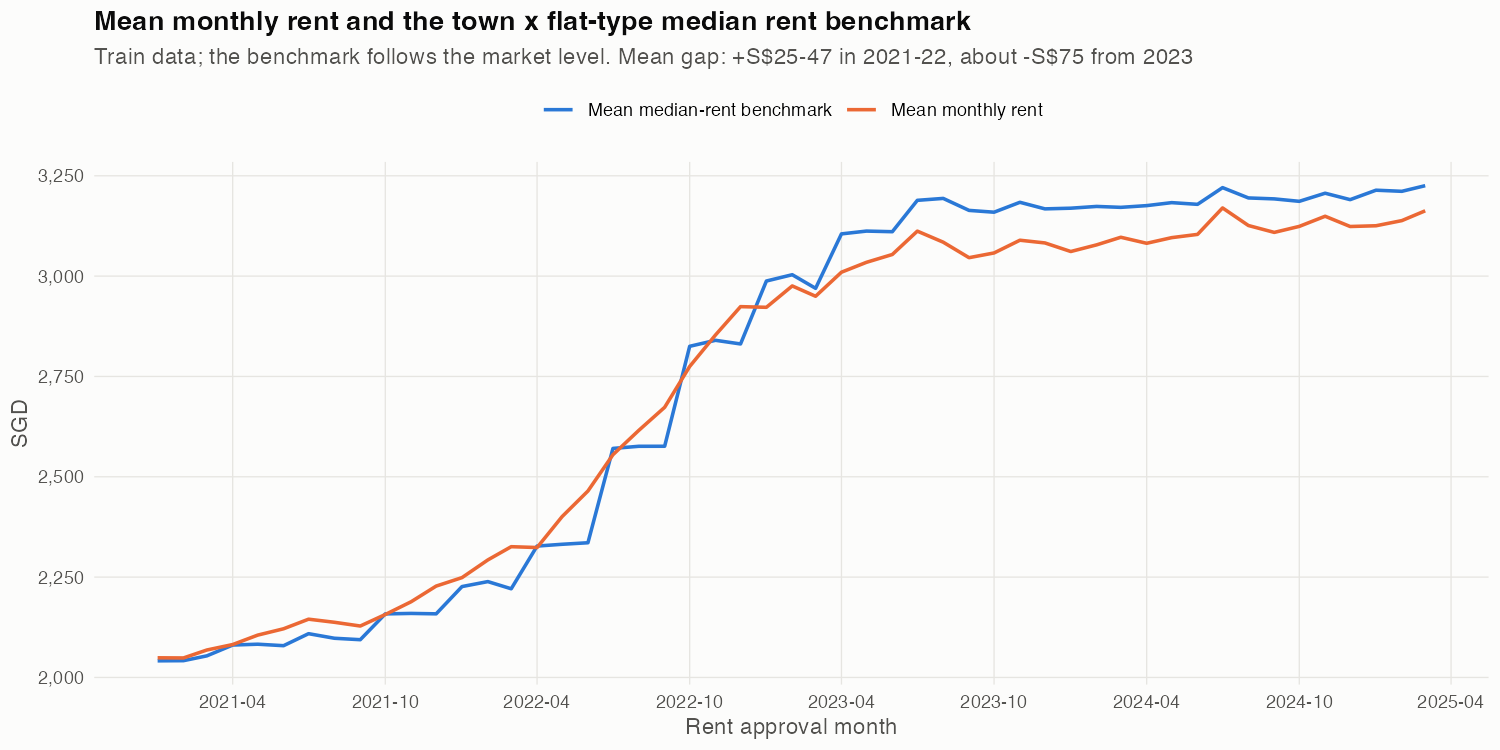
\includegraphics[width=\columnwidth]{../beina/figures/trend_rent_vs_benchmark.png}
\caption{Mean monthly rent and the mean town $\times$ flat-type median benchmark (train months).\src{Be-trend}}\label{fig:trend}
\end{figure}

\subsection{Calendar and macro proxies}
Approval date, COE premium and stock prices correlate strongly with rent over the whole period only because they share the trend. COE correlates 0.898 with monthly mean rent in levels but 0.015 in month-on-month changes.\src{Be-coe} Inside the validation period their rank correlation with rent collapses (COE 0.528 to 0.006, approval date 0.562 to 0.018), whereas the town $\times$ flat-type historical mean keeps 0.664 to 0.668 (Fig.~\ref{fig:assoc}).\src{Me-assoc} Mutual information with rent likewise ranks that historical mean first (0.361), ahead of approval date (0.229) and COE premium (0.218).\src{Me-mi} COE and stocks have negative permutation importance ($-0.08$, $-0.06$) and are dropped.\src{Be-imp} A random split would hide this failure, so all validation is chronological.

\begin{figure}[t]
\centering
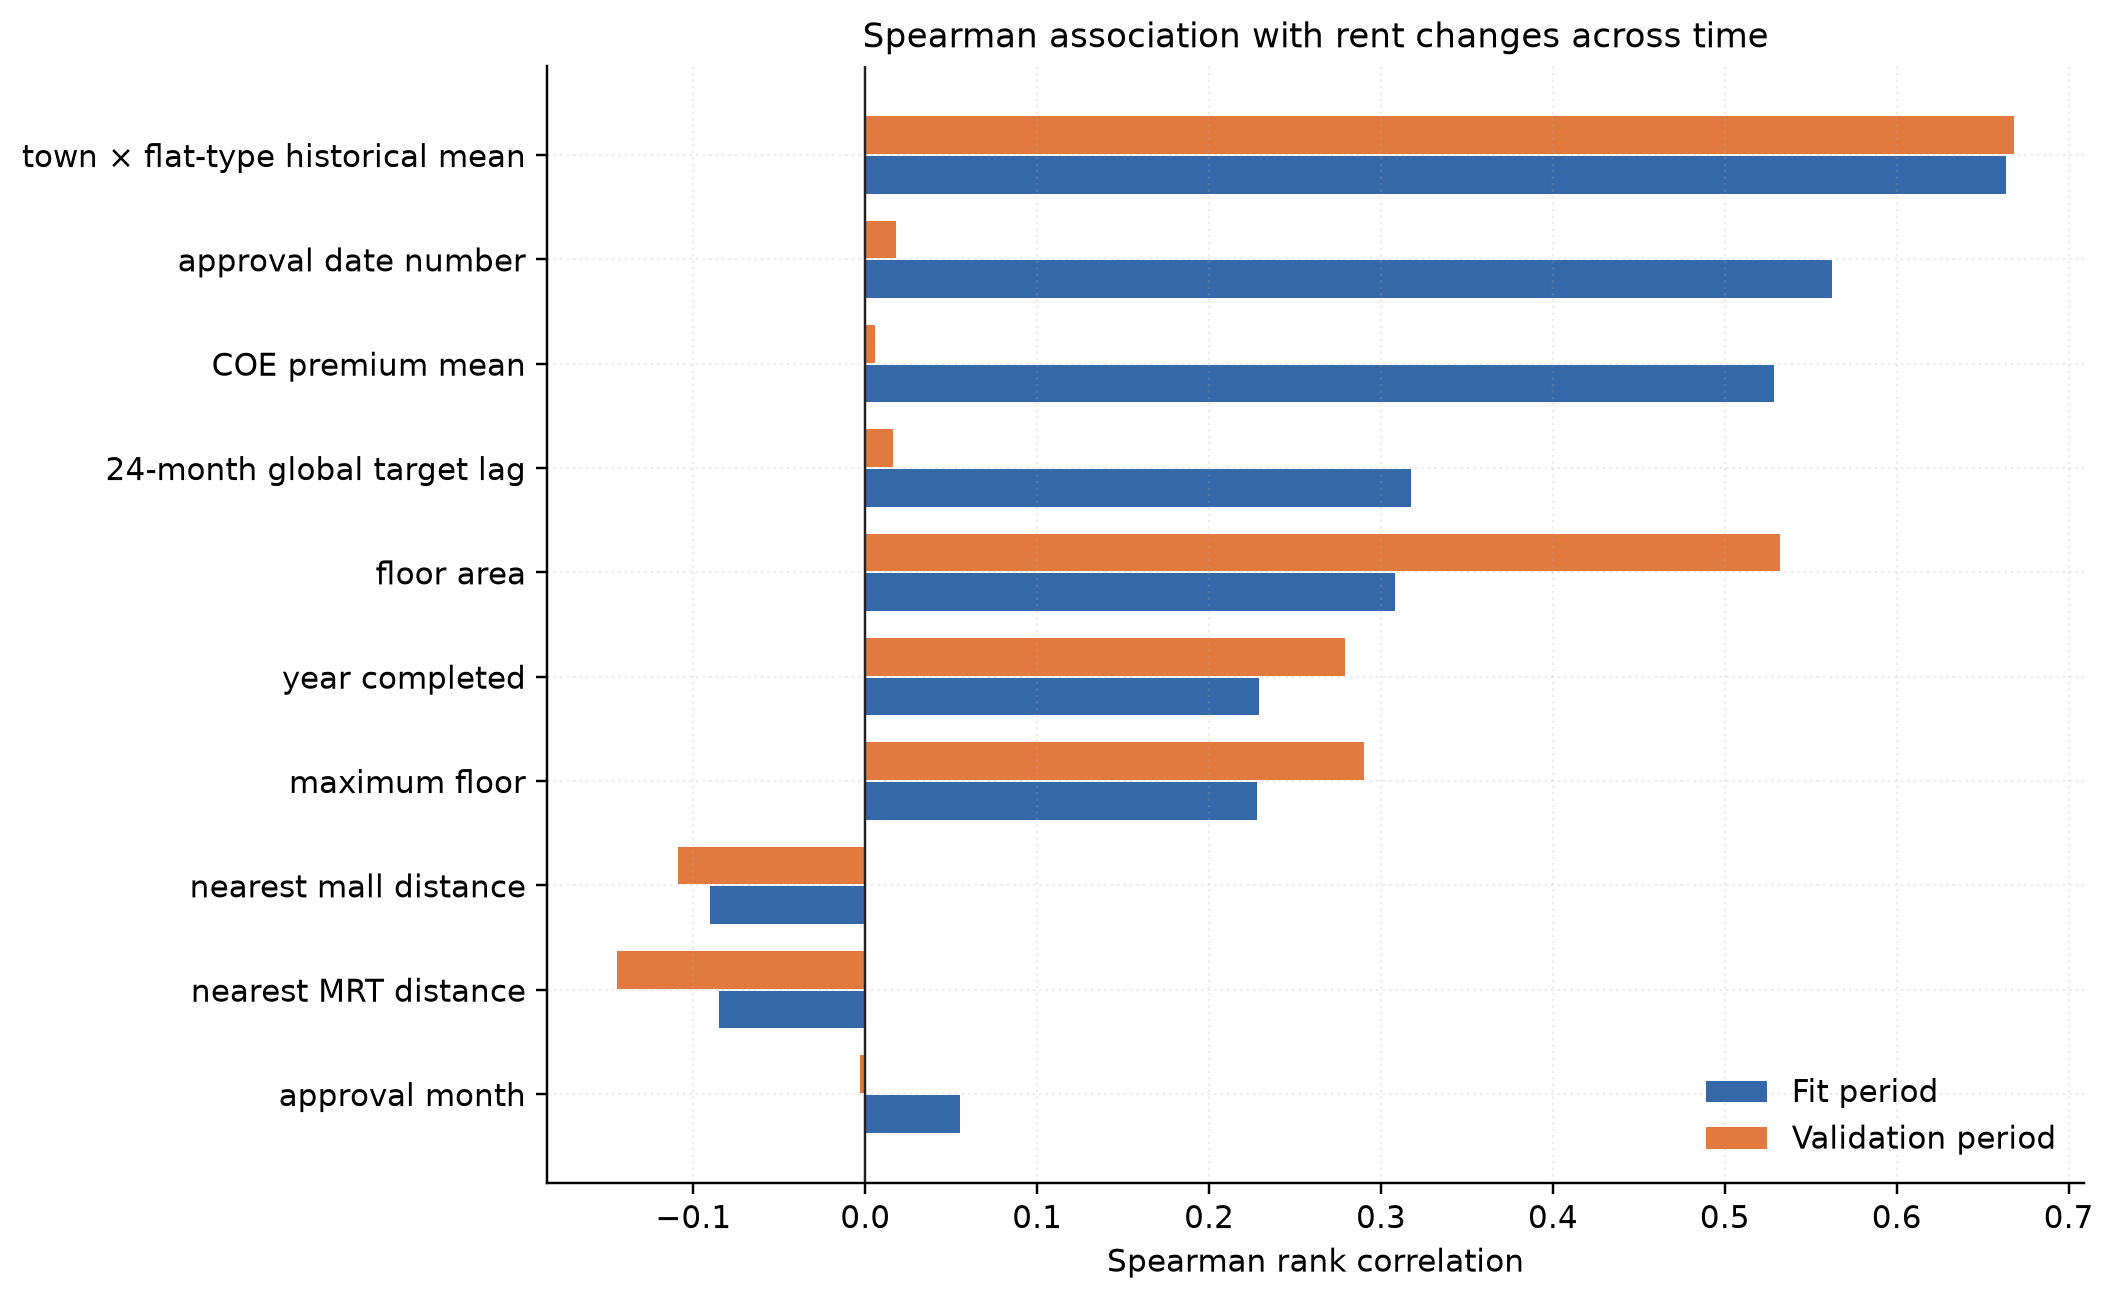
\includegraphics[width=\columnwidth]{../metul/figures/association_stability.png}
\caption{Spearman correlation with rent in the fitting and chronological validation periods (P1 protocol).\src{Me-assoc}}\label{fig:assoc}
\end{figure}

\subsection{Location, categories and outliers}
Once the benchmark is removed the numeric features correlate weakly with the residual ($|r|\le 0.12$), so the remainder is mostly block-level.\src{Be-weakcorr} Shuffling the seven target encodings (mostly block-level) raises out-of-time RMSE by 40.4, the largest effect of any feature group; the four location encodings alone account for 34.2.\src{Be-imp}

Lowercasing and normalising separators cuts \texttt{STREET} from 1,146 to 576 values and \texttt{FLAT\_TYPE} from 11 to 6.\src{Me-cat} Every test town, street, flat type and model occurs in training; 11 unseen block labels affect 36 of 50,000 test rows (0.072\%).\src{Me-cov} Without normalising address casing, 30,781 train rows (20.5\%) fail to join to the block table.\src{Be-join} Eleven blocks store $-1$ for maximum floor and year completed (159 train rows) and are imputed; one median entry (300 against about 3,000 elsewhere) is removed.\src{Be-sent,Be-bad}

We keep every row. The IQR rule flags 130 floor areas and 752 rents,\src{Me-out} but only 0.11\% of rows are extreme relative to their benchmark. The highest rents are real adjoined flats and premium maisonettes, the lowest (\sgd 300--450) are 2-room flats that are probably subsidised or room rentals.\src{Be-out} Removing training tails also hurt RMSE at every level we tried (Section~\ref{sec:matter}).

\begin{figure}[t]
\centering
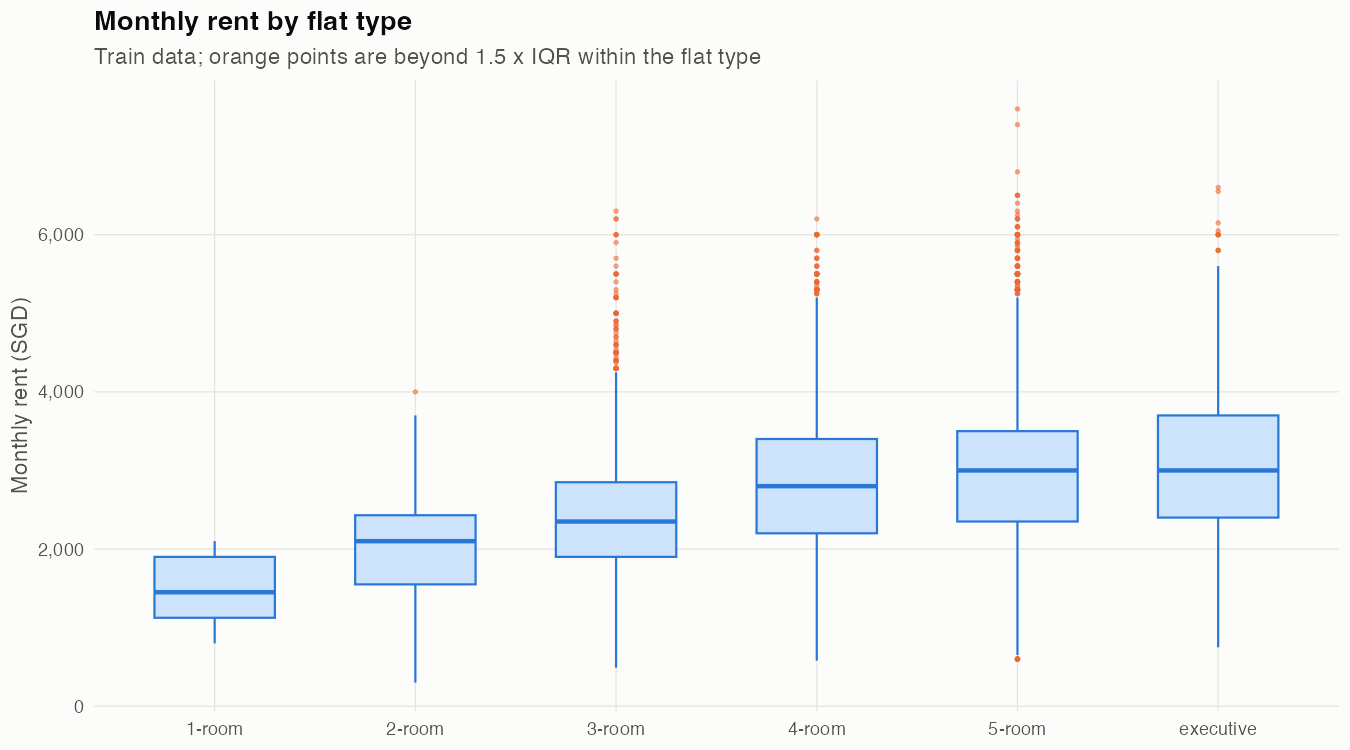
\includegraphics[width=\columnwidth]{../beina/figures/outlier_box_flat_type.png}
\caption{Monthly rent by flat type; points beyond $1.5\times$IQR within the type are shown but kept.\src{Be-out}}\label{fig:box}
\end{figure}

\subsection{Noise floor}
Rows sharing every model input get the same prediction from any deterministic model, so rent spread inside such groups is irreducible. Three groupings give similar estimates: SD 461 for same-unit rentals in one quarter;\src{Be-noise} 464.0 over all labelled months and 454.8 on window P1 for groups sharing all eight inputs;\src{Pu-noise} and 464 for flats in one block, type and month, covering 26.8\% of rows.\src{Aa-noise} Rents are also rounded (87.5\% end in 00), which adds to the noise.\src{Be-round} Our local RMSE of about 450 is of the same order. These estimates cover only rows with a twin and exclude test-period noise.\src{Pu-noise-limit}

\section{Preprocessing and Features}
Table~\ref{tab:eda2prep} traces each exploratory finding to the preprocessing decision it motivated; the pipeline is in Fig.~\ref{fig:flow}.

\begin{table*}[t]
\caption{From exploratory findings to preprocessing decisions.}\label{tab:eda2prep}
\centering\footnotesize
\begin{tabular}{@{}p{5.9cm}p{5.9cm}p{3.6cm}@{}}
\toprule
Finding & Decision & Evidence\\
\midrule
Rent up 53\% then flat; trees cannot extrapolate & Predict the residual over an official median; chronological validation only & Sec.~II-B, Table~\ref{tab:base}\\
COE, stocks and date share only the trend & Drop COE and stocks; never validate on random splits & Sec.~II-C\\
Block-level premiums dominate the residual & Nested shrinkage encodings for block, street and subzone & Table~\ref{tab:imp}\\
Spelling variants (\texttt{STREET} 1,146 to 576 values) & Normalise strings; use native categoricals & Sec.~II-D\\
Sentinel $-1$ values; one bad median entry & Impute from block statistics; remove the entry & Sec.~II-D\\
Outliers are real units and the test set has similar rows & Keep every row; no tail trimming & Sec.~II-D, Table~\ref{tab:matter}\\
Rents rounded; identical flats differ in rent & Treat as a noise floor; do not chase sub-point gains & Sec.~II-E\\
Published medians cover the test quarters & Honest anchor: frozen at 2025-Q1 plus drift & Sec.~III-B, Table~\ref{tab:honest}\\
\bottomrule
\end{tabular}
\end{table*}

\begin{figure*}[t]
\centering
\resizebox{0.98\textwidth}{!}{%
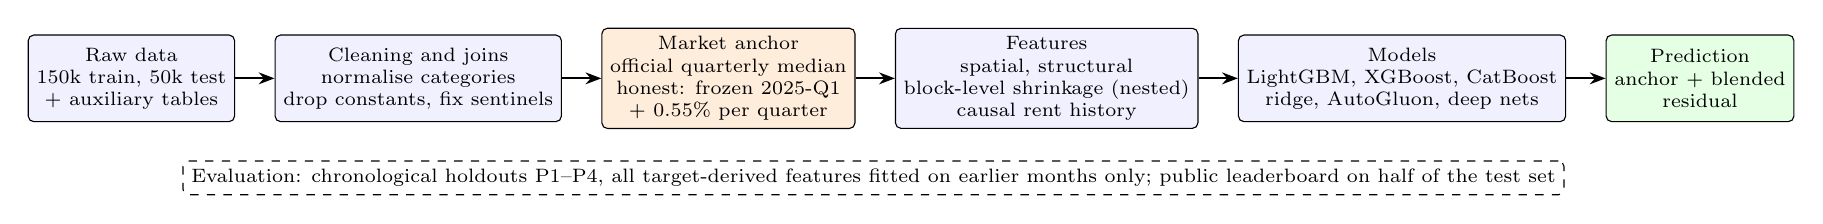
\begin{tikzpicture}[node distance=5mm,
 box/.style={draw,rounded corners=2pt,align=center,minimum height=11mm,font=\scriptsize,fill=blue!6,inner sep=3pt},
 arr/.style={-{Stealth[length=2mm]},thick}]
\node[box] (raw) {Raw data\\150k train, 50k test\\+ auxiliary tables};
\node[box,right=of raw] (clean) {Cleaning and joins\\normalise categories\\drop constants, fix sentinels};
\node[box,right=of clean,fill=orange!14] (anchor) {Market anchor\\official quarterly median\\honest: frozen 2025-Q1\\+ 0.55\% per quarter};
\node[box,right=of anchor] (feat) {Features\\spatial, structural\\block-level shrinkage (nested)\\causal rent history};
\node[box,right=of feat] (model) {Models\\LightGBM, XGBoost, CatBoost\\ridge, AutoGluon, deep nets};
\node[box,right=of model,fill=green!10] (out) {Prediction\\anchor + blended\\residual};
\draw[arr] (raw)--(clean); \draw[arr] (clean)--(anchor); \draw[arr] (anchor)--(feat); \draw[arr] (feat)--(model); \draw[arr] (model)--(out);
\node[draw,dashed,rounded corners=2pt,font=\scriptsize,align=center,below=4mm of feat,xshift=-2.2cm,inner sep=3pt] (ev) {Evaluation: chronological holdouts P1--P4, all target-derived features fitted on earlier months only; public leaderboard on half of the test set};
\end{tikzpicture}}
\caption{Design shared by the four pipelines. The anchor and its honest variant are the central design choice.}\label{fig:flow}
\end{figure*}

\subsection{Cleaning and leakage control}
Rental and block strings are lowercased, trimmed and joined on town, block and street; after normalisation every train and test row matches exactly one block.\src{Be-join} Every target-derived feature for a row in month $t$ uses only labels from months before $t$,\src{Pu-leak} and encoders are fitted inside each training split with inner five-fold out-of-fold values so a row's rent never enters its own feature.\src{Be-te-leak}

\subsection{Market anchor and its honest variant}
The target is rent minus the official median rent for the row's town, flat type and quarter; predictions add it back. Because 51.8\% of the table's values are missing, a fallback chain fills each row: its own cell (96.6\% of train rows), then the national median for the flat type (3.3\%), then adjacent quarters.\src{Be-anchor}

The file runs to 2026-Q2, but a quarter's median aggregates that quarter's rents, so values after the last labelled quarter feed test-period information into the anchor.\src{Be-leak} Our first submission (V2) used them.\src{Aa-v2anchor} The honest variant freezes each cell at 2025-Q1 and multiplies by $\exp(g\,k)$ for $k$ quarters ahead, where $g$ is the mean quarterly log growth of a national index over the last four quarters (+0.55\% at 2025-Q1).\src{Be-drift} Our implementation reproduces the published drift values (+0.78\% at 2024-Q2, +0.55\% at 2025-Q1).\src{Aa-drift}

\subsection{Block-level shrinkage encodings}
High-cardinality keys (14,828 block $\times$ flat-type levels, 576 streets) are encoded by empirical-Bayes shrinkage~\cite{micci}\src{Aa-fp,Me-cat} toward their parent key:
\begin{equation}
\hat\mu_k=\frac{n_k\,\bar r_k+M\,\hat\mu_{\mathrm{parent}(k)}}{n_k+M},\label{eq:te}
\end{equation}
where $\bar r_k$ is the mean residual of key $k$. The hierarchy is town ($M{=}30$), block ($10$), block $\times$ flat type ($5$), street ($15$), subzone ($20$).\src{Aa-M} The R pipeline uses the same constants for the shared levels.\src{Be-te} Hand-set constants proved near-optimal: a random-effects fit recovered 16 for street and 21 for subzone (against 15 and 20) and gave no reliable gain elsewhere.\src{Aa-gpb}

\subsection{Other features}
Structural features (floor area, area per room, maximum floor, year completed, flat age) and distances to the nearest MRT station, mall, school and the CBD with counts within radii\src{Be-spatial} are common to all pipelines. In the V2 pipeline these are computed once per unique block with scikit-learn \texttt{BallTree} indexes under the Haversine metric: nearest distance and counts within 0.5, 1 and 2~km for MRT stations (all, operating, planned, multi-line interchange), malls and primary, secondary and top-tier schools, 20 features in all, including inverse-distance proximity scores.\src{Aa-ball} The R pipeline computes the same kinds of distances independently. The history pipeline adds a 24-month global rent lag and smoothed town $\times$ flat-type and block $\times$ flat-type means with counts; removing the property-level history raises RMSE by 4.388.\src{Pu-hist,Pu-hist-abl} The earlier single-LightGBM root pipeline adds an address-level trailing rent per square metre, which lowers its validation RMSE from 456.70 to 452.56.\src{Aa-addr} The AutoGluon pipeline adds nearest-place names.\src{Me-feat}

\section{Data Mining Methods}
\subsection{Models}
Tabular data with mixed numeric and high-cardinality categorical inputs and 150,000 rows suits boosted trees; trees remain strongest on medium-sized tabular data~\cite{grinsztajn}, and under time-based splits gradient-boosted trees and embedding MLPs rank best~\cite{tabred}. We use LightGBM~\cite{lightgbm}, XGBoost~\cite{xgboost} and CatBoost~\cite{catboost} (ordered target statistics), ridge regression, FT-Transformer~\cite{ftt}, TabTransformer~\cite{tabt}, MLPs, a Temporal Fusion Transformer~\cite{tft} for segment-level forecasts, neural gates and segmented models. The AutoGluon pipeline's AutoGluon-Tabular~\cite{autogluon} setup restricts its base models to LightGBM and CatBoost; AutoGluon's second-level weighted ensemble learns global blend weights, unlike the input-dependent neural gates tested separately, and is extended in later experiments with stacked residual layers. We also reproduced a delayed neural network for Singapore housing prices~\cite{wang2016}.\src{Me-families,Be-paper} Empirical-Bayes target encoding~\cite{micci} and its regularised, cross-fitted forms~\cite{pargent} are standard for high-cardinality keys; random-effects boosting~\cite{gpboost} is the likelihood-based counterpart, which we test in Section~\ref{sec:matter}.

\textbf{Categorical handling.} Categoricals are passed natively to the tree learners; this beat one-hot encoding in six of seven configurations (town, region and block: 481.89 against 482.09),\src{Me-onehot} and replacing every categorical by its target mean was 6.1 to 10.7 RMSE worse.\src{Me-te-all} In the AutoGluon pipeline's selected configuration, automatic text feature generation is disabled with the \texttt{ignore\_text} preset. Thus fields such as street and nearest-MRT name remain categorical, without automatically generated text-special or n-gram columns.\src{Me-text} Encodings of block-like keys are the exception, because they carry information no other feature has (Table~\ref{tab:imp}). Missing numeric block attributes fall back to the town--street median, then the town median, then the global median.\src{Me-fallback}

\subsection{Automated Feature-Selection Experiments}
After establishing a compact manual subset of structurally meaningful property, time, location and accessibility variables, the AutoGluon pipeline evaluated automated selection on a broader 36-variable pool. Two wrapper methods were tested: permutation-importance recursive feature elimination (RFE), which repeatedly refitted the LightGBM--CatBoost ensemble before removing weak variables, and SHAP ranking followed by top-$k$ refits. Chronological rank correlation, mutual information and matched ablations provided supporting diagnostics rather than full-period correlation alone. PCA and truncated SVD were used only as diagnostics because their leading components were not temporally stable. Test labels were never used for selection.\src{Me-fs-manual,Me-fs-auto,Me-dim}

\subsection{Choice of baseline for the residual}
A residual target only helps if the baseline carries the right level. Table~\ref{tab:base} compares baselines across pipelines. A national-level baseline, even an oracle one that knows the actual national average, is worse than the official town $\times$ flat-type median,\src{Be-two-stage} and the history pipeline's residual over a global 24-month lag collapses (CatBoost 662.5 against 464.2 for direct prediction) because the lag lacks town and flat-type detail.\src{Pu-lagres} An explicit trend-plus-residual network is likewise weaker than direct deep prediction (518.6 against 495.9).\src{Me-trendres} Predicting a ratio instead of a difference gave no gain (change $-0.02$).\src{Be-impr}

\begin{table}[t]
\caption{Baselines for the residual target (RMSE).\src{Be-two-stage,Pu-lagres}}\label{tab:base}
\centering\footnotesize
\begin{tabular}{@{}p{4.6cm}p{2.9cm}@{}}
\toprule
Baseline (protocol) & RMSE\\
\midrule
Town $\times$ flat-type official median (P2) & 452.19\\
National level, last 3 months carried forward & 461.99\\
National level, oracle (actual average) & 459.07\\
National level, linear trend & 556.33\\
\midrule
Global 24-month lag, LightGBM / CatBoost (P1): residual & 646.6 / 662.5\\
\hspace{1.2em}same models, direct prediction & 470.8 / 464.2\\
\bottomrule
\end{tabular}
\end{table}

\subsection{Hyperparameters}
The V2 pipeline fixes its settings (LightGBM 1,200 trees, 75 leaves, rate 0.04, early stopping on each fold's validation split).\src{Aa-hp} The R pipeline ran 12, 10 and 6-trial random searches for LightGBM, XGBoost and CatBoost;\src{Be-hp} the history pipeline fixed three LightGBM capacities and three CatBoost seeds and early-stops on the validation window;\src{Pu-hp} the AutoGluon pipeline used 25 trials per model family, supplying the validation period as tuning data.\src{Me-hpo} On the root pipeline a grid, two random searches and a 100-trial Optuna~\cite{optuna} search all fell inside the cross-validation noise: Optuna's best configuration scored 453.71 against 452.56 for the shipped one.\src{Aa-optuna}

\subsection{Blending and final system}
Weights are fitted on out-of-fold or validation predictions: SLSQP in the V2 pipeline (0.545, 0.075, 0.380 for LightGBM, XGBoost, CatBoost),\src{Aa-w} softmax-constrained in the R pipeline,\src{Be-blend} non-negative bounded to $[0,0.85]$ in the history pipeline.\src{Pu-blend}

\textbf{Final models.} We selected two final submissions. The first is five-fold bagged LightGBM, XGBoost and CatBoost on the residual over the \emph{honest} anchor, with the weights above. It scored 433.65480 on the public leaderboard, 0.048 above the version that used published test-quarter medians.\src{Aa-final,Aa-honest-lb} The second is the R pipeline's honest-anchor blend, the version its report adopts; the same setup with COE and stocks scored 433.89670, and the final run without them had not been scored when that report was written.\src{Be-final}

\section{Evaluation and Interpretation}
\subsection{Protocols}
The pipelines used different chronological splits (Table~\ref{tab:proto}); scores compare only within a protocol. Early stopping, candidate selection and blend weights use the validation labels in every pipeline, so local scores are model-selection scores, not untouched estimates; only the leaderboard is independent, and it covers half the test rows.\src{Pu-sel,Me-sel} RMSE is the competition metric; differences are tested with a paired bootstrap that resamples block--month groups (300 draws in the V2 pipeline; 2,000 group resamples in the history pipeline) because rows in one group share unit-level noise.\src{Aa-boot,Pu-noise}

\begin{table}[t]
\caption{Validation protocols.}\label{tab:proto}
\centering\footnotesize
\begin{tabular}{@{}llp{4.6cm}@{}}
\toprule
ID & Pipelines & Fit / validate\\
\midrule
P1 & AutoGluon, history & before 2024-05 (117,988) / 2024-05 to 2025-03 (32,012)\src{Me-split,Pu-W}\\
P2 & V2, R & through 2024-06 (124,016) / 2024-07 to 2025-03 (25,984)\src{Be-split,Aa-e2split}\\
P3 & V2, history (W2) & before 2024-10 (132,802) / 2024-10 to 2025-03 (17,198); the root pipeline drops 641 duplicate rows\src{Pu-W,Aa-dup}\\
P4 & V2 & through 2023-11 / 2023-12 to 2025-03 (16 months)\src{Aa-honest-cost}\\
\bottomrule
\end{tabular}
\end{table}

\subsection{Model comparison}
Table~\ref{tab:results} gives representative results. On P1 the boosted-tree ensemble with causal rent history (463.2) beats AutoGluon without HPO (467.1) by 4 RMSE, and every deep model, gate or router is worse: the best deep expert scores 477.0, TabTransformer 495.9, and segmenting by town or flat type loses 4.6 to 7.6 against the global control.\src{Pu-me,Me-res,Me-seg} On P2 the anchor-and-encoding recipe reaches 450--452 with published medians and 454.9 with the honest anchor, and the R pipeline gives 449.65 and 454.72.\src{Be-res,Aa-honest-cost} On P3, the V2-recipe LightGBM scores 443.64 against 448.688 for the history pipeline's detailed LightGBM, but the first uses published medians and the second none, so the two are not like-for-like.\src{Aa-tab,Pu-w2} A Temporal Fusion Transformer forecasts town $\times$ flat-type monthly means well (RMSE 258.453, $R^2$ 0.8400 on 1,340 segment-months), but adding a listing-level residual model is worse than predicting listings directly (499.791 against 471.209).\src{Me-tft}

\begin{table}[t]
\caption{Representative local RMSE (SGD) by protocol. $^\dagger$published medians; $^\ddagger$honest anchor.\src{Aa-tab,Be-res,Me-res,Pu-me,Pu-w2}}\label{tab:results}
\centering\footnotesize
\begin{tabular}{@{}l@{\hspace{4pt}}l@{\hspace{4pt}}p{3.2cm}r@{}}
\toprule
Prot. & Pipeline & Model & RMSE\\
\midrule
P1 & History & CatBoost, best single seed & 463.549\\
P1 & History & blend v2 / + \sgd/sqm model (v3) & 463.155 / 462.906\\
P1 & AutoGluon & 18 features, no HPO & 467.122\\
P1 & AutoGluon & + one weighted residual layer & 468.057\\
P1 & AutoGluon & deep experts: best / equal blend & 476.979 / 471.168\\
P1 & AutoGluon & TabTransformer & 495.853\\
P2 & R & ridge / LightGBM$^\dagger$ & 451.95 / 452.29\\
P2 & R & XGBoost / CatBoost$^\dagger$ & 450.97 / 450.27\\
P2 & R & blend$^\dagger$ / blend$^\ddagger$ (3 seeds) & 449.65 / 454.72\\
P2 & V2 & CatBoost / LightGBM$^\dagger$ & 450.43 / 452.48\\
P2 & V2 & blend 0.2/0.8$^\dagger$ / blend$^\ddagger$ & 450.30 / 454.85\\
P3 & History & blend v2 / detailed LightGBM & 443.3 / 448.688\\
P3 & V2 & LightGBM$^\dagger$ & 443.64\\
\bottomrule
\end{tabular}
\end{table}

\subsection{Automated Feature-Selection Results}
The controlled manual screen selected a compact 13-variable subset at RMSE 467.230, ahead of the 31-variable full table at 467.507 and the 25-variable candidate expansion at 468.304. The selected production representation subsequently extended the compact set with a prior-only town $\times$ flat-type mean, a global 24-month rent lag and three nearest-place names; its default LightGBM--CatBoost ensemble scored 467.122. Because training budgets and automatic text handling differed between these stages, the latter comparison is a development progression rather than a pure one-variable ablation.\src{Me-fs-manual}

Automated reduction did not establish a stronger independent result. RFE retained all 36 candidates at 468.921; reducing to 10 produced 469.080, while intermediate subsets were less stable. Under the same shortened protocol, the SHAP top-18 subset scored 467.841 against 468.272 for the manual 18-variable set. This 0.431 improvement was selected on the same outer validation period, so it was not treated as an untouched estimate and did not replace the production representation. PCA showed the same temporal-instability warning: the first numeric component's target correlation fell from 0.654 in fitting to 0.306 in validation, and no PCA/SVD replacement-model RMSE was recorded.\src{Me-fs-auto,Me-dim}

\begin{table}[t]
\caption{Automated Feature-selection results on P1.\src{Me-fs-manual,Me-fs-auto}}\label{tab:feature-selection}
\centering\footnotesize
\begin{tabular}{@{}p{2.0cm}p{3.9cm}r@{}}
\toprule
Method & Selected / matched comparator & RMSE\\
\midrule
Manual subsets & Compact 13 / full 31 & 467.230 / 467.507\\
RFE & All 36 / reduced 10 & 468.921 / 469.080\\
SHAP top-$k$ & Top 18 / manual 18 & 467.841 / 468.272\\
\bottomrule
\end{tabular}
\end{table}

\subsection{Alternative Modelling Approaches}
Table~\ref{tab:alternatives} compares the principal alternatives evaluated in the AutoGluon pipeline on the common P1 listing holdout.
Hard segmentation did not help: routing AutoGluon by town and flat type scored 475.846 and 476.068, against global controls of 468.272 and 471.448.
The same pattern held for random forests: the global model scored 484.923, flat-type routing scored 486.073, and chronological tuning improved the global forest to 479.319 but left it well behind boosted trees.
Splitting the data therefore lost more shared signal than it gained from local specialisation.\src{Me-seg,Me-alt}

Deep tabular models learned useful structure but remained weaker than tree ensembles. The best individual deep expert, 
an FT-Transformer, scored 476.979; TabTransformer scored 495.853, while averaging three deep experts improved to 471.168. 
A block-to-town neural gate scored 475.130, so input-dependent routing was again inferior to a fixed blend. The standalone FT-Transformer run scored 497.497, 
and an explicit neural trend-plus-residual decomposition scored 518.590.\src{Me-res,Me-trendres,Me-alt}

Asymmetric and residual-specialist models also showed the value of shrinkage. Quantile LightGBM at $q{=}0.60$ reduced MAE from 356.438 to 343.087 
and shifted predictions toward over-forecasting, but worsened RMSE from 478.370 to 492.281. Weighted flat-type residual experts 
made a small improvement over their matched Layer-1 control (468.272 to 468.068); the significant-residual gate scored 468.360 and the unweighted segmented correction 
deteriorated to 472.509. Thus residual models helped only when their corrections were strongly attenuated.\src{Me-alt}

Time-series experiments used different targets or holdouts and are not included in Table~\ref{tab:alternatives}. A property-group time-series ensemble scored 477.592 
on observed item-months. A town $\times$ flat-type market forecast reached 273.240 at segment level, but its listing hybrid scored 486.052. Likewise, TFT reached 258.453 on segment-month means, 
yet TFT plus a listing residual scored 499.791 against 471.209 for direct listing prediction. Under rolling-origin evaluation, an explicit trend-plus-residual model scored 571.673 against 567.562 for the direct baseline. 
Aggregate temporal patterns were learnable, but their errors compounded when forecasts were translated back to individual listings.\src{Me-tft,Me-alt}

\begin{table}[t]
\caption{Alternative listing-level models evaluated using validation RMSE under the P1 protocol.\src{Me-res,Me-seg,Me-alt}}\label{tab:alternatives}
\centering\scriptsize
\begin{tabular}{@{}p{1.45cm}p{5.05cm}r@{}}
\toprule
Approach & Model description & P1 RMSE\\
\midrule
Reference & AutoGluon LightGBM--CatBoost, default settings & \textbf{467.122}\\
Residual specialists & Weighted flat-type residual experts & 468.068\\
 & Significant-residual gated specialist & 468.360\\
Fixed / learned blends & Equal LightGBM--CatBoost blend & 468.740\\
 & Equal deep-expert blend & 471.168\\
 & Neural LightGBM--CatBoost gate & 472.274\\
 & Block-to-town deep gate & 475.130\\
Hard segmentation & Town-routed AutoGluon & 475.846\\
 & Flat-type-routed AutoGluon & 476.068\\
Random forests & Chronologically tuned random forest & 479.319\\
 & Global random forest & 484.923\\
 & Flat-type-routed random forest & 486.073\\
Asymmetric loss & Quantile LightGBM ($q{=}0.60$) & 492.281\\
Deep tabular & TabTransformer & 495.853\\
 & FT-Transformer & 497.497\\
\bottomrule
\end{tabular}
\end{table}

\subsection{What mattered and what did not}\label{sec:matter}
Table~\ref{tab:matter} separates the changes that moved the score from those that did not. The anchor is decisive over a long horizon: on P4 it cuts RMSE from 600.72 to 492.77, while on a 6-month window the gain is not significant.\src{Aa-anchor} Target encodings, mostly at block level, are the other component that matters: removing all seven costs 8.68 RMSE for the blend and 19.47 for ridge,\src{Be-te-abl} and the step from V1 to V2, which added hierarchical encodings (and interchange-distance features), is the only visible jump on the leaderboard (Fig.~\ref{fig:lb}).\src{Aa-lb} Almost everything else lies within about one RMSE or is worse. Tuning moves results by under 1.2 in the R pipeline's experiments, and recency weighting is reliably worse because it discards block information.\src{Be-impr} Table~\ref{tab:imp} shows where the signal sits: the encodings dominate, the benchmark features come next, and COE and stocks contribute nothing.

\begin{table}[t]
\caption{Permutation importance by feature group: increase in out-of-time RMSE when shuffled (CatBoost, R pipeline).}\label{tab:imp}
\centering\footnotesize
\begin{tabular}{@{}lr@{\hspace{1.4em}}lr@{}}
\toprule
Group & $\Delta$ & Group & $\Delta$\\
\midrule
All 7 encodings & +40.4 & Flat model & +2.1\\
Location encodings & +34.2 & MRT & +1.4\\
Benchmark features & +13.1 & Time & +0.1\\
Flat age, lease year & +6.2 & Stocks & $-0.06$\\
CBD distance & +5.7 & COE & $-0.08$\\
\bottomrule
\end{tabular}\src{Be-imp}
\end{table}

\begin{table*}[t]
\caption{Effect of changes on RMSE (positive = worse). CI = paired-bootstrap 95\% interval; n.s. = not significant.}\label{tab:matter}
\centering\footnotesize
\begin{tabular}{@{}p{5.8cm}p{5.6cm}p{4.0cm}@{}}
\toprule
Change & Effect & Where measured\\
\midrule
Residual over anchor, long horizon & 600.72 $\to$ 492.77\src{Aa-anchor} & P4, root pipeline\\
Residual over anchor, 6-month window & 452.56 $\to$ 451.87 (CI $-1.98$ to $+0.52$, n.s.)\src{Aa-anchor} & P3, root pipeline\\
Target encodings removed (7 keys, mostly block-level) & +8.68 blend, +19.47 ridge\src{Be-te-abl} & P2 (R)\\
Property-level rent history removed & +4.388\src{Pu-hist-abl} & P1 (history)\\
Address-level trailing feature added & $-4.14$ (456.70 $\to$ 452.56)\src{Aa-addr} & P3, root pipeline\\
\midrule
Optuna, 100 trials, vs shipped configuration & +1.15 (453.71 vs 452.56)\src{Aa-optuna} & P3, root pipeline\\
Huber, Fair, L1 losses (Huber $\delta{=}1000$ ties) & +0.7 to +4.9\src{Aa-robust} & P2, P4\\
Trimming 0.5--2.5\% from each tail & +1.7 to +10.6\src{Aa-trim} & P2, P4\\
Random-effects model (GPBoost) replacing encodings & +5.26 and +7.98\src{Aa-gpb} & P2, P4\\
External resale premium by block / neighbour-block priors & $-0.56$, $-0.15$ (n.s.) / $-0.25$ (n.s.), +0.82\src{Aa-resale} & P2, P4\\
Neural gate vs equal blend; town / flat-type routing & +3.5; +7.6 / +4.6\src{Me-res,Me-seg} & P1 (AutoGluon)\\
Prediction-as-feature second layer; AdaBoost residual & +69.9; +29.1\src{Me-stack} & P1 (AutoGluon)\\
Recency weighting (24-month half-life) & +1.14\src{Be-impr} & P2 (R)\\
CatBoost-heavy blend weights & $-0.51$ / $-1.09$ locally, public score +0.023\src{Aa-cbw,Aa-lb} & P2, P4; leaderboard\\
Honest instead of published anchor & +4.55 (P2), public score +0.048\src{Aa-honest-cost,Aa-honest-lb} & P2; leaderboard\\
\bottomrule
\end{tabular}
\end{table*}

\subsection{Local gains against the leaderboard}
Fig.~\ref{fig:lb} shows every submission. The anchor-and-encoding pipelines, the causal-history pipeline and the AutoGluon LightGBM--CatBoost stack fall within 433.4 to 436.3, a plateau only 0.7\% wide. Three local gains of 0.5 to 3 RMSE (deeper trees, premium and bagging, CatBoost-heavy weights) did not appear on the leaderboard (434.05, 434.03, 433.63 against V2's 433.61),\src{Aa-lb,Aa-cbw,Aa-trim} consistent with the public score covering half the test rows and unit-level noise dominating.\src{Pu-lb-limit} Published studies find public leaderboards rank reliably despite adaptive reuse~\cite{roelofs} but that tiny differences carry little information~\cite{ladder}.

\begin{figure}[t]
\centering
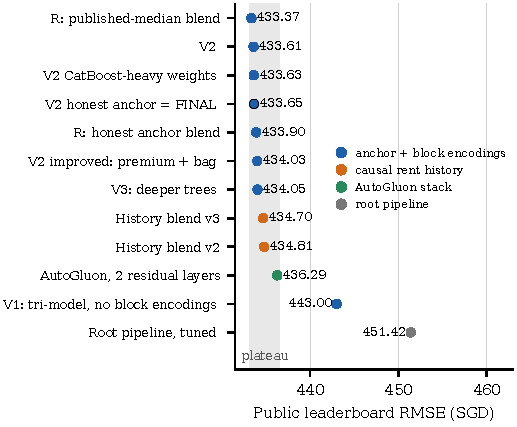
\includegraphics[width=\columnwidth]{figures/fig_leaderboard.pdf}
\caption{Public leaderboard RMSE of every submission by pipeline. The final model is outlined.\src{Aa-lb,Be-lb,Pu-lb,Me-lb}}\label{fig:lb}
\end{figure}

\subsection{Honest anchor}
Table~\ref{tab:honest} quantifies the cost of removing test-period information on the V2 recipe. On P2 it is 4.6 to 6.3 RMSE, matching the R pipeline's measurement of about 5 locally and 0.5 on the leaderboard.\src{Aa-honest-cost,Be-honest-lb} Drift helps when the market is flat (mean error falls from +47.6 to +1.8) but is catastrophic after a surge: at the 2023-Q3 cutoff $g$ was +5.05\% per quarter and extrapolating it over six quarters over-predicted by 885 by 2025-Q1. At the true cutoff $g$ is only +0.55\%, the flat case. The same fragility appears in the history pipeline's backtests, where projected market indices help in one regime and hurt in another.\src{Pu-backtest}

\begin{table}[t]
\caption{Anchor variants, blend 0.2 LightGBM / 0.8 CatBoost (RMSE).\src{Aa-honest-cost}}\label{tab:honest}
\centering\footnotesize
\begin{tabular}{@{}lccc@{}}
\toprule
Holdout & Published & Frozen & Frozen + drift\\
\midrule
P2 ($g{=}{+}0.78\%$) & 450.30 & 456.57 & 454.85\\
P4 ($g{=}{+}5.05\%$) & 482.53 & 487.48 & 764.71\\
\bottomrule
\end{tabular}
\end{table}

\subsection{Data volume and recency}
More real data helps much more than tuning: RMSE falls by roughly 6 to 8 per doubling of training rows (465.77 at 13k rows to 443.64 at 133k) with no sign of saturation, and training that ends 9, 12 or 15 months earlier costs 0.92, 1.84 and 4.17 against a same-size recent sample (Fig.~\ref{fig:learn}).\src{Aa-learn} Block premiums are estimated from few transactions (about 8 rows per block-type level), which is the likely reason for the appetite for data. This also explains why synthetic rows cannot help: the gain comes from real transactions at specific blocks.

\begin{figure}[t]
\centering
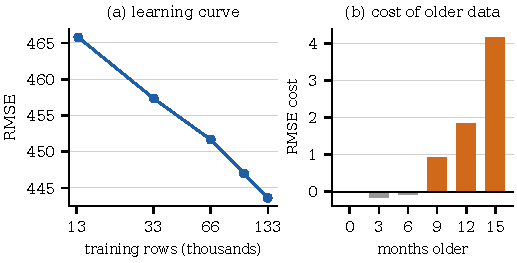
\includegraphics[width=\columnwidth]{figures/fig_learning.pdf}
\caption{(a) RMSE against training rows for V2's recipe on the 2024-10 to 2025-03 window; (b) cost of training data that ends earlier, against a same-size sample.\src{Aa-learn}}\label{fig:learn}
\end{figure}

\subsection{Where the model fails}
Error is concentrated (Fig.~\ref{fig:resid}). On the root pipeline the 6.5\% of validation rows with rent at or below \sgd 2,100 have RMSE 1,090 against 370 for the rest, and so carry 37.5\% of the squared error.\src{Aa-tail} The AutoGluon pipeline's out-of-fold diagnostics show the same pattern by segment: executive flats have RMSE 720, five-room 653 and three-room 542.\src{Me-seg-err} Within a block, flat type and month, rents differ with SD 464, so most of this is not recoverable from the available columns.\src{Aa-noise} The history pipeline finds that on rows with an exact twin, RMSE (452.8) lies inside the interval for the noise estimate (442.2 to 466.8), and that rows without a twin score 14.1 worse, which noise and headroom cannot separate.\src{Pu-twin} Table~\ref{tab:backtest} shows the level error in a rising market. A model that ignores the market also lags: in a rising-market backtest the history pipeline under-predicts by 312 on average, and supplying the true index cuts RMSE from 629.9 to 500.2.\src{Pu-backtest}

\begin{table}[t]
\caption{Moving-market backtests of the history pipeline: 12-month windows after each origin, LightGBM fitted on all earlier rows. Bias is prediction minus actual; the oracle index deflates the target by a market index that includes the validation months.}\label{tab:backtest}
\centering\footnotesize
\begin{tabular}{@{}lccc@{}}
\toprule
Origin & 2022-01 & 2023-01 & 2024-01\\
\midrule
Rent change & +30.0\% & +5.5\% & +2.0\%\\
Control RMSE & 629.9 & 629.1 & 493.9\\
Control bias & $-312.2$ & $-152.0$ & +14.2\\
Oracle RMSE & 500.2 & 604.6 & 490.6\\
Noise SD & 471.3 & 588.5 & 479.3\\
\bottomrule
\end{tabular}\src{Pu-backtest}
\end{table}

\begin{figure}[t]
\centering
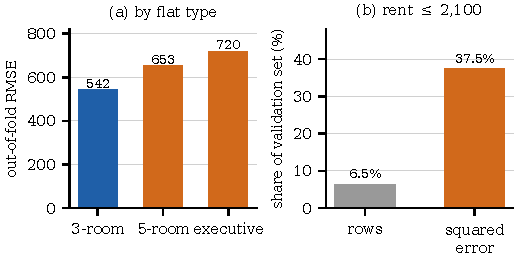
\includegraphics[width=\columnwidth]{figures/fig_errors.pdf}
\caption{Where the error sits: (a) out-of-fold RMSE by flat type (AutoGluon pipeline); (b) the 6.5\% of validation rows with rent at or below \sgd 2,100 carry 37.5\% of the squared error (root pipeline).\src{Me-seg-err,Aa-tail}}\label{fig:resid}
\end{figure}

\textbf{Answers to the research questions.} \textbf{Q1:} the official town $\times$ flat-type median as a residual baseline, with block-level shrinkage encodings, carries the level: public RMSE 443.0 to 433.6 and, over a 16-month holdout, 600.72 to 492.77.\src{Aa-lb,Aa-anchor} \textbf{Q2:} almost nothing else adds more than about one RMSE (Table~\ref{tab:matter}), although more real data does help (Fig.~\ref{fig:learn}). \textbf{Q3:} identical flats differ with SD 455--464 against our local RMSE of about 450, so little headroom remains.\src{Pu-noise,Aa-noise} \textbf{Q4:} local gains of 0.5 to 3 did not reach the leaderboard, and the honest anchor costs 4.6 locally but 0.05 publicly, so local protocols both over- and under-state differences; paired intervals and the leaderboard should be read together.\src{Aa-lb,Aa-honest-cost,Aa-honest-lb}

\section{Limitations and Future Work}
\textbf{Evaluation.} Every local score reuses validation labels for selection;\src{Pu-sel} protocols differ across pipelines; and the test-period market level is unmeasured, since the history pipeline's leaderboard shift probe was never scored.\src{Pu-probe} \textbf{Anchor.} The published medians leak test-period aggregates; our honest variant costs little on the leaderboard but its drift rule is regime-dependent. \textbf{Information.} No dataset we could use legitimately separates units within a block: the official rental registry carries the same fields as ours and the target itself, which is why we did not use it, and block-level data cannot tell two flats in one block apart.\cite{hdbrent} Resale-derived signals and neighbour-block priors gave under one RMSE.\src{Aa-resale} \textbf{Future work:} unit-level data (floor, condition) if the course permits it, regime-aware drift selection, recency-aware encodings, and uncertainty estimates for the heavy low-rent tail.

\textbf{Conclusion.} Carrying the market level through an official median anchor and shrinking block-level premiums toward their parents account for the only large gain we found; everything built on top sits inside a noise floor of about 455--464 SGD that our three groupings measure consistently. The honest forecast-time version of the same model scores 433.65480.

\begin{thebibliography}{99}
\bibitem{hdbrent} Housing and Development Board, ``Renting out of flats,'' data.gov.sg, \url{https://data.gov.sg/dataset/renting-out-of-flats}, accessed Oct. 2026.
\bibitem{grinsztajn} L. Grinsztajn, E. Oyallon and G. Varoquaux, ``Why do tree-based models still outperform deep learning on typical tabular data?'' in \emph{Proc. NeurIPS}, 2022.
\bibitem{tabred} I. Rubachev \emph{et al.}, ``TabReD: Analyzing pitfalls and filling the gaps in tabular deep learning benchmarks,'' in \emph{Proc. ICLR}, 2025.
\bibitem{lightgbm} G. Ke \emph{et al.}, ``LightGBM: A highly efficient gradient boosting decision tree,'' in \emph{Proc. NeurIPS}, 2017.
\bibitem{xgboost} T. Chen and C. Guestrin, ``XGBoost: A scalable tree boosting system,'' in \emph{Proc. KDD}, 2016.
\bibitem{catboost} L. Prokhorenkova \emph{et al.}, ``CatBoost: Unbiased boosting with categorical features,'' in \emph{Proc. NeurIPS}, 2018.
\bibitem{autogluon} N. Erickson \emph{et al.}, ``AutoGluon-Tabular: Robust and accurate AutoML for structured data,'' arXiv:2003.06505, 2020.
\bibitem{ftt} Y. Gorishniy, I. Rubachev, V. Khrulkov and A. Babenko, ``Revisiting deep learning models for tabular data,'' in \emph{Proc. NeurIPS}, 2021.
\bibitem{tabt} X. Huang, A. Khetan, M. Cvitkovic and Z. Karnin, ``TabTransformer: Tabular data modeling using contextual embeddings,'' arXiv:2012.06678, 2020.
\bibitem{tft} B. Lim, S. {\"O}. Ar{\i}k, N. Loeff and T. Pfister, ``Temporal fusion transformers for interpretable multi-horizon time series forecasting,'' \emph{Int. J. Forecasting}, vol. 37, no. 4, pp. 1748--1764, 2021.
\bibitem{wang2016} L. Wang, F. F. Chan, Y. Wang and Q. Chang, ``Predicting public housing prices using delayed neural networks,'' in \emph{Proc. IEEE TENCON}, 2016, pp. 3589--3592.
\bibitem{micci} D. Micci-Barreca, ``A preprocessing scheme for high-cardinality categorical attributes in classification and prediction problems,'' \emph{ACM SIGKDD Explor.}, vol. 3, no. 1, pp. 27--32, 2001.
\bibitem{optuna} T. Akiba, S. Sano, T. Yanase, T. Ohta and M. Koyama, ``Optuna: A next-generation hyperparameter optimization framework,'' in \emph{Proc. KDD}, 2019.
\bibitem{pargent} F. Pargent, F. Pfisterer, J. Thomas and B. Bischl, ``Regularized target encoding outperforms traditional methods in supervised machine learning with high cardinality features,'' \emph{Computational Statistics}, 2022, arXiv:2104.00629.
\bibitem{gpboost} F. Sigrist, ``Gaussian process boosting,'' \emph{J. Mach. Learn. Res.}, vol. 23, no. 232, pp. 1--46, 2022.
\bibitem{roelofs} R. Roelofs \emph{et al.}, ``A meta-analysis of overfitting in machine learning,'' in \emph{Proc. NeurIPS}, 2019.
\bibitem{ladder} A. Blum and M. Hardt, ``The Ladder: A reliable leaderboard for machine learning competitions,'' in \emph{Proc. ICML}, 2015.
\end{thebibliography}

\clearpage
\appendices
\section{Workload}\label{app:work}
\begin{table}[h]
\centering\footnotesize
\begin{tabular}{@{}lp{6.0cm}@{}}
\toprule
Member & Main responsibility\\
\midrule
Aayush & Root pipeline and data-quality audit; median-rent residual anchor and its honest forecast-time variant; V2 recipe (hierarchical shrinkage encodings, BallTree spatial features, three-model blend) and leaderboard series; final submission and the end-to-end reproducible \texttt{main.py}; ablations (tail trimming, robust losses, GPBoost, resale, learning curve)\\
Metul & Shared preprocessing; association, mutual-information and PCA analysis; AutoGluon, deep tabular, gating, segmentation, time-series and residual-stack experiments\\
Punyaa & Leakage-safe causal rent-history features; LightGBM/CatBoost ensemble and 76 unit tests; extrapolation, noise-floor and moving-market backtests\\
Beina & R cleaning and EDA; in-fold hierarchical encodings; honest-anchor drift; ablations and feature importance; the second selected final submission (\texttt{predict\_test.R})\\
\bottomrule
\end{tabular}
\end{table}
\emph{This table summarises the content of each member's folder under \texttt{report/}; each member should confirm it.}\src{Wk-P,Wk-M,Wk-B}

\section{Hyperparameters and reproduction}
V2: LightGBM 1,200 trees, 75 leaves, learning rate 0.04, subsample 0.8, column sample 0.75; XGBoost depth 7; CatBoost 1,200 iterations, depth 7, learning rate 0.05; early stopping 40 rounds; five folds, seed 42.\src{Aa-v2hp} The final model is reproduced end to end, from the raw files to \url{submission.csv}, by \url{main.py} with the code in \url{modules/}.\src{Aa-main} Experiment scripts: \url{expt-2/src/models_v2.py} (V2), \url{expt-5/src/honest_v2_submission.py} (honest anchor), \url{expt-5/src/exp6_honest_anchor_validation.py} (Table~\ref{tab:honest}). History pipeline: \url{python3 -m punyaa.train}; R pipeline: \url{model_training.R}, \url{predict_test.R}; AutoGluon pipeline: notebooks under \url{exploration/metul}.\src{Pu-repro,Be-scripts,Me-trace}

\end{document}
"  to show them, plain  pdflatex main  hides them ----
\newif\ifshowsrc
\ifdefined\SHOWSRC\showsrctrue\else\showsrcfalse\fi
\newcommand{\src}[1]{\ifshowsrc\textsuperscript{\tiny\color{gray}[#1]}\fi}

\newcommand{\sgd}{S\$}
\def\BibTeX{{\rm B\kern-.05em{\sc i\kern-.025em b}\kern-.08em T\kern-.1667em\lower.7ex\hbox{E}\kern-.125emX}}

\begin{document}
\pagestyle{plain}
\pagenumbering{arabic}

\title{Forecasting HDB Rents Sixteen Months Ahead:\\Market Anchors, Block-Level Shrinkage and the Noise Floor\\[2pt]\large Team 2 --- [TEAM NAME]}

\author{\IEEEauthorblockN{Aayush Majumdar}
\IEEEauthorblockA{\textit{Student ID A0352046L}\\
\textit{National University of Singapore}}
\and
\IEEEauthorblockN{Metul Prabhu}
\IEEEauthorblockA{\textit{Student ID A0352394Y}\\
\textit{National University of Singapore}}
\and
\IEEEauthorblockN{Punyaa [Surname]}
\IEEEauthorblockA{\textit{Student ID [ID]}\\
\textit{National University of Singapore}}
\and
\IEEEauthorblockN{Beina [Surname]}
\IEEEauthorblockA{\textit{Student ID [ID]}\\
\textit{National University of Singapore}}}

\maketitle
\thispagestyle{plain}

\begin{abstract}
We forecast the monthly rent of 50,000 Singapore HDB flat rentals approved up to sixteen months after our 150,000 labelled examples (2021--2025). We built four pipelines on the same data: gradient-boosted trees on the residual over an official median rent with block-level shrinkage encodings, causal rent-history features, AutoGluon LightGBM--CatBoost stacks plus deep tabular models, and an R pipeline with the first design. Three findings emerge. First, predicting the residual over the official median rent, with block-level encodings, is the only change that moved the public leaderboard materially (443.0 to 433.6 RMSE). Second, deep models, gating, segmentation, hyperparameter search, robust losses, tail trimming and external resale data each moved RMSE by about one point or made it worse. Third, identical flats rent with a standard deviation of about 455--464 SGD, the same order as our error. The released median-rent file covers the test quarters and so leaks future aggregates; an honest forecast-time anchor costs about 5 RMSE locally but 0.05 on the leaderboard. Our final model scores 433.65480.\src{Aa-lb,Aa-honest-lb,Aa-honest-cost,Be-noise,Pu-noise,Aa-noise,Me-families}
\end{abstract}

\section{Introduction}
Rents of public housing are a visible measure of living costs, and the Housing and Development Board (HDB) publishes every approved flat rental as open data~\cite{hdbrent}. A model that predicts a flat's rent helps tenants and owners judge asking rents and helps analysts follow the market. We predict the monthly rent of 50,000 rental approvals dated March 2025 to July 2026 from 150,000 labelled approvals dated January 2021 to March 2025, plus auxiliary tables on blocks, MRT stations, malls, schools, COE premiums, stock prices and official median rents.\src{Pu-task,Be-inputs}

Three properties make the task hard. (i) The test months lie up to sixteen months after the last label,\src{Pu-future} while rents rose 53\% over the labelled period and then flattened.\src{Be-trend} (ii) Location carries most of the signal at a finer grain than any single numeric feature.\src{Be-weakcorr} (iii) Flats that look identical in the data rent for different amounts.\src{Pu-noise}

We ask four questions. \textbf{Q1:} what information lets a model carry the market level to unseen months? \textbf{Q2:} how much can better models add on top? \textbf{Q3:} how much of the error is irreducible? \textbf{Q4:} how far can local validation be trusted against an external leaderboard? We call the four pipelines V2 (boosted trees on the residual over the official median), R (the same design in R), history (causal rent-history features) and AutoGluon (stacks and deep tabular models).

\section{Data and Exploratory Analysis}
\subsection{Data}
Table~\ref{tab:data} lists the inputs. Only eight raw columns vary (approval month, town, block, street, flat type, flat model, floor area, lease start); \texttt{FURNISHED} and \texttt{FEE} are constant and are dropped.\src{Pu-task}

\begin{table}[t]
\caption{Data used.}\label{tab:data}
\centering\footnotesize
\begin{tabular}{@{}p{2.3cm}p{5.2cm}@{}}
\toprule
File & Content\\
\midrule
train / test & 150,000 rentals (2021-01 to 2025-03) / 50,000 (2025-03 to 2026-07)\src{Be-inputs}\\
HDB blocks & 9,464 blocks: coordinates, maximum floor, year completed, subzone\src{Be-inputs}\\
MRT, malls, schools & 243 stations, 113 malls, 337 schools\src{Be-inputs}\\
COE, stocks & monthly premiums, daily prices (tested, not retained)\\
Median rent & 13,305 quarterly values by town and flat type, 51.8\% missing\src{Be-anchor}\\
\bottomrule
\end{tabular}
\end{table}

\subsection{Market drift}
Mean rent rose 53\%, from \sgd 2,055 (first three months) to \sgd 3,142 (last three), nearly all of it between mid-2021 and mid-2023; it has been almost flat since.\src{Be-trend} The official town $\times$ flat-type median follows the level closely (Fig.~\ref{fig:trend}). Trees cannot extrapolate a trend,\src{Pu-trees} so every strong model here predicts the residual over this benchmark instead of rent itself.

\begin{figure}[t]
\centering
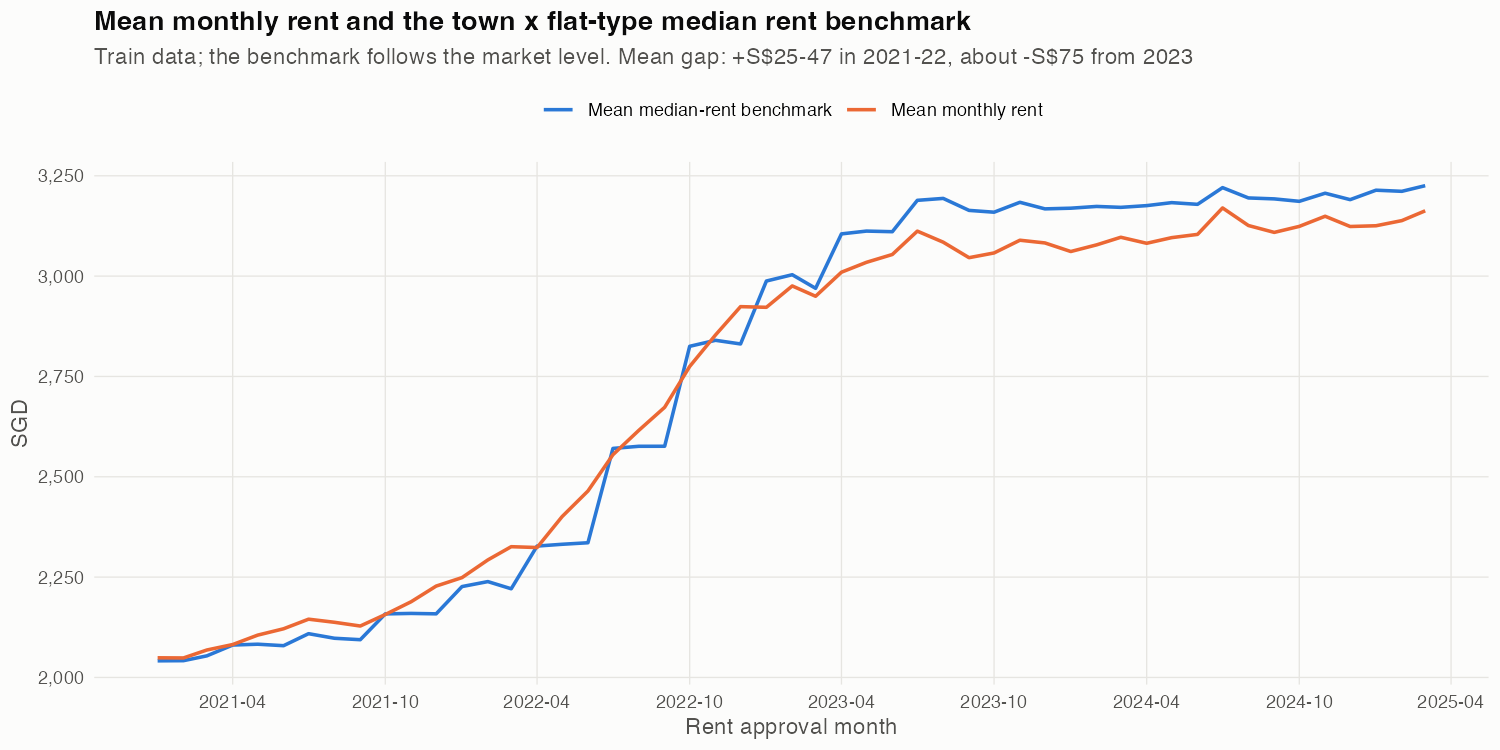
\includegraphics[width=\columnwidth]{../beina/figures/trend_rent_vs_benchmark.png}
\caption{Mean monthly rent and the mean town $\times$ flat-type median benchmark (train months).\src{Be-trend}}\label{fig:trend}
\end{figure}

\subsection{Calendar and macro proxies}
Approval date, COE premium and stock prices correlate strongly with rent over the whole period only because they share the trend. COE correlates 0.898 with monthly mean rent in levels but 0.015 in month-on-month changes.\src{Be-coe} Inside the validation period their rank correlation with rent collapses (COE 0.528 to 0.006, approval date 0.562 to 0.018), whereas the town $\times$ flat-type historical mean keeps 0.664 to 0.668 (Fig.~\ref{fig:assoc}).\src{Me-assoc} Mutual information with rent likewise ranks that historical mean first (0.361), ahead of approval date (0.229) and COE premium (0.218).\src{Me-mi} COE and stocks have negative permutation importance ($-0.08$, $-0.06$) and are dropped.\src{Be-imp} A random split would hide this failure, so all validation is chronological.

\begin{figure}[t]
\centering
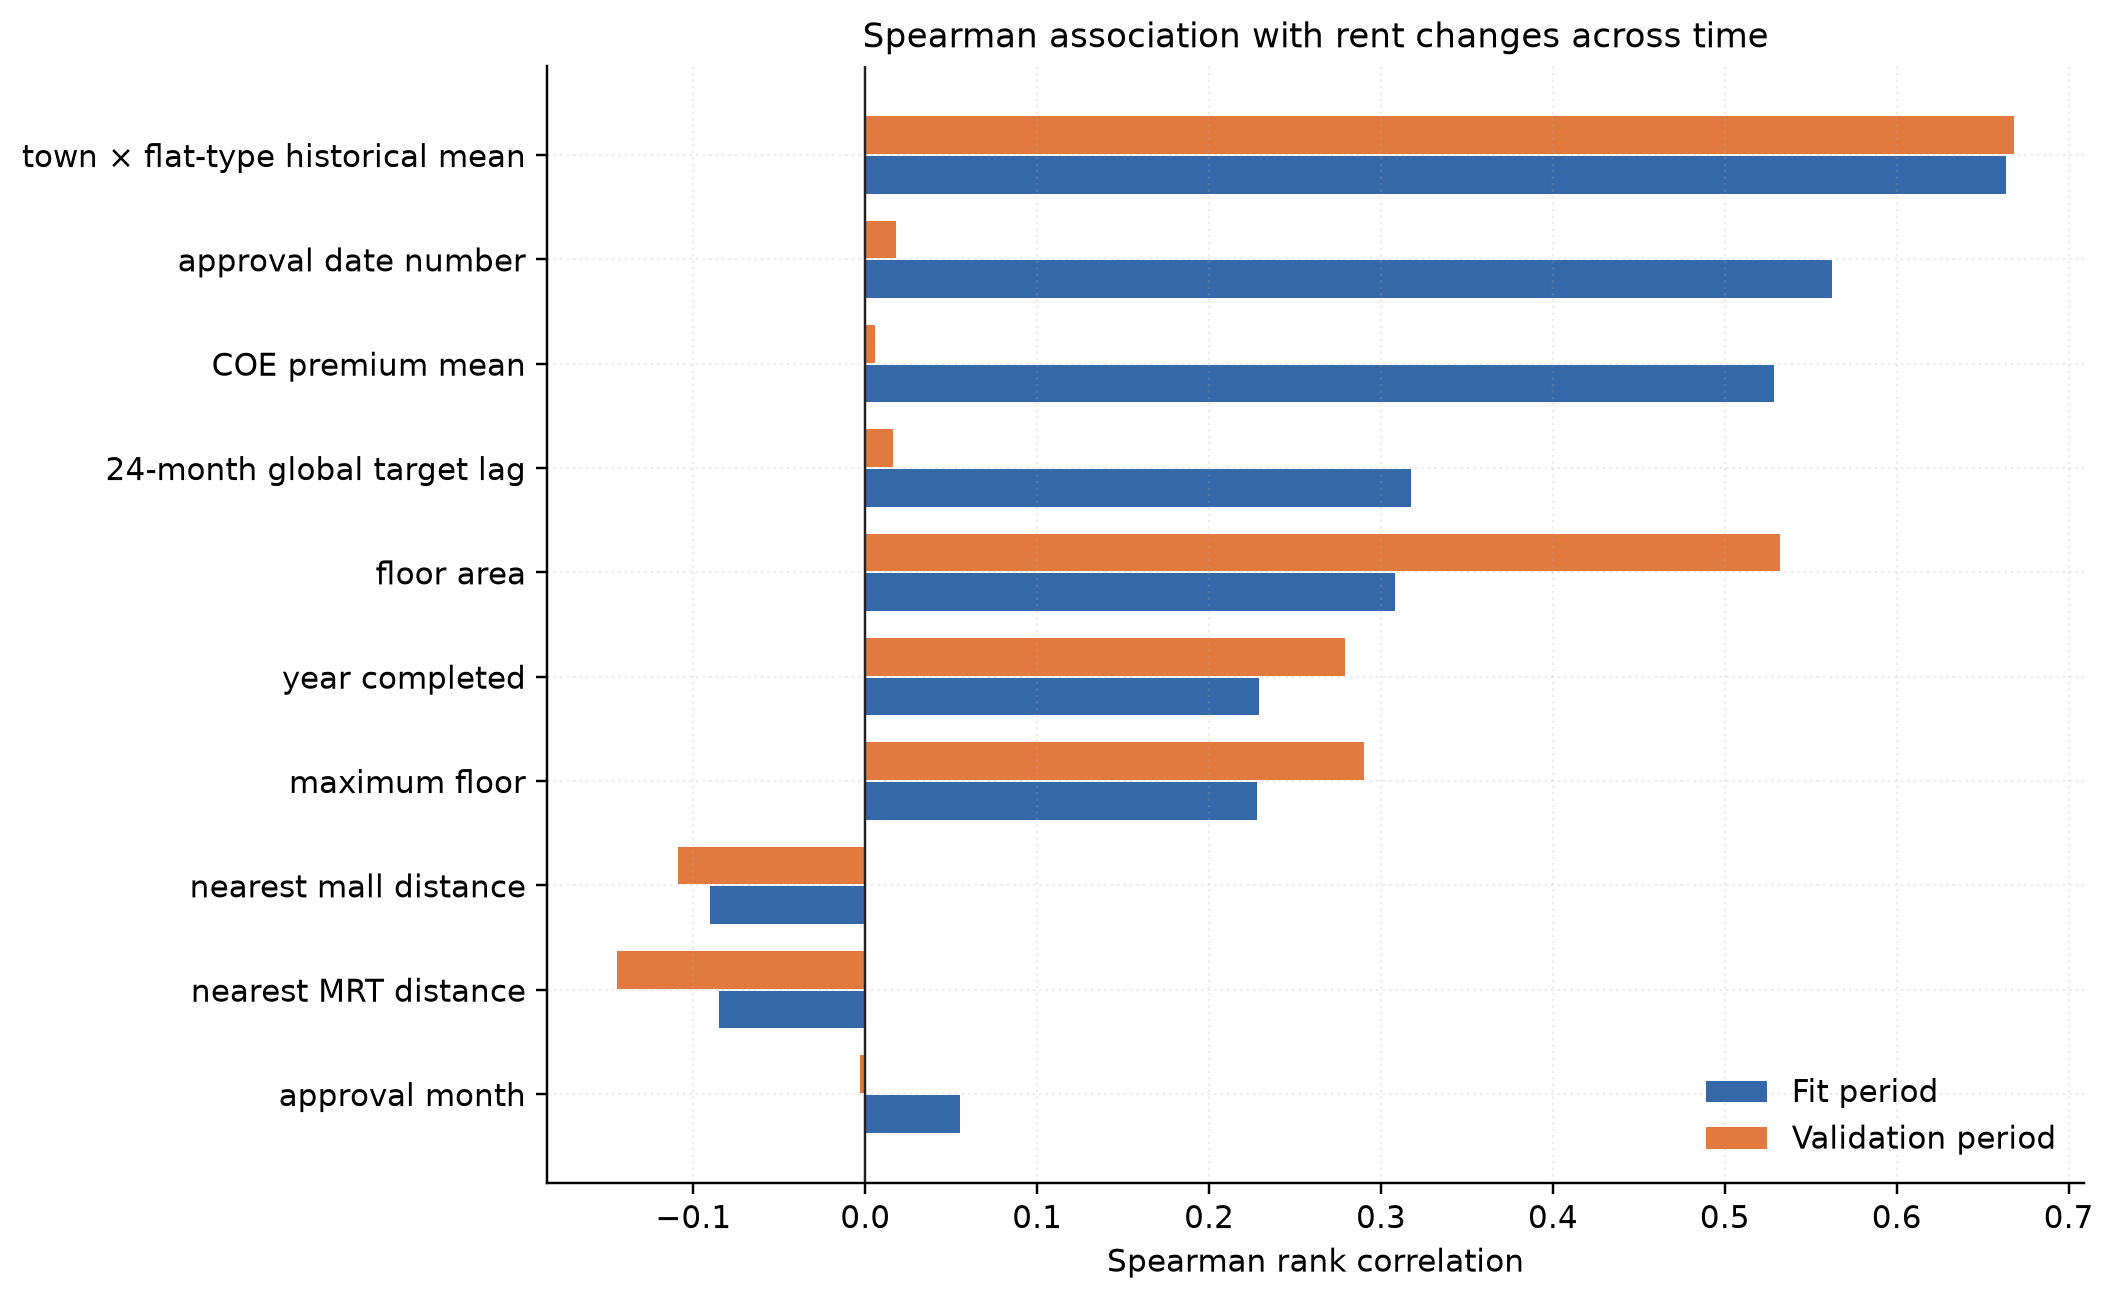
\includegraphics[width=\columnwidth]{../metul/figures/association_stability.png}
\caption{Spearman correlation with rent in the fitting and chronological validation periods (P1 protocol).\src{Me-assoc}}\label{fig:assoc}
\end{figure}

\subsection{Location, categories and outliers}
Once the benchmark is removed the numeric features correlate weakly with the residual ($|r|\le 0.12$), so the remainder is mostly block-level.\src{Be-weakcorr} Shuffling the seven target encodings (mostly block-level) raises out-of-time RMSE by 40.4, the largest effect of any feature group; the four location encodings alone account for 34.2.\src{Be-imp}

Lowercasing and normalising separators cuts \texttt{STREET} from 1,146 to 576 values and \texttt{FLAT\_TYPE} from 11 to 6.\src{Me-cat} Every test town, street, flat type and model occurs in training; 11 unseen block labels affect 36 of 50,000 test rows (0.072\%).\src{Me-cov} Without normalising address casing, 30,781 train rows (20.5\%) fail to join to the block table.\src{Be-join} Eleven blocks store $-1$ for maximum floor and year completed (159 train rows) and are imputed; one median entry (300 against about 3,000 elsewhere) is removed.\src{Be-sent,Be-bad}

We keep every row. The IQR rule flags 130 floor areas and 752 rents,\src{Me-out} but only 0.11\% of rows are extreme relative to their benchmark. The highest rents are real adjoined flats and premium maisonettes, the lowest (\sgd 300--450) are 2-room flats that are probably subsidised or room rentals.\src{Be-out} Removing training tails also hurt RMSE at every level we tried (Section~\ref{sec:matter}).

\begin{figure}[t]
\centering
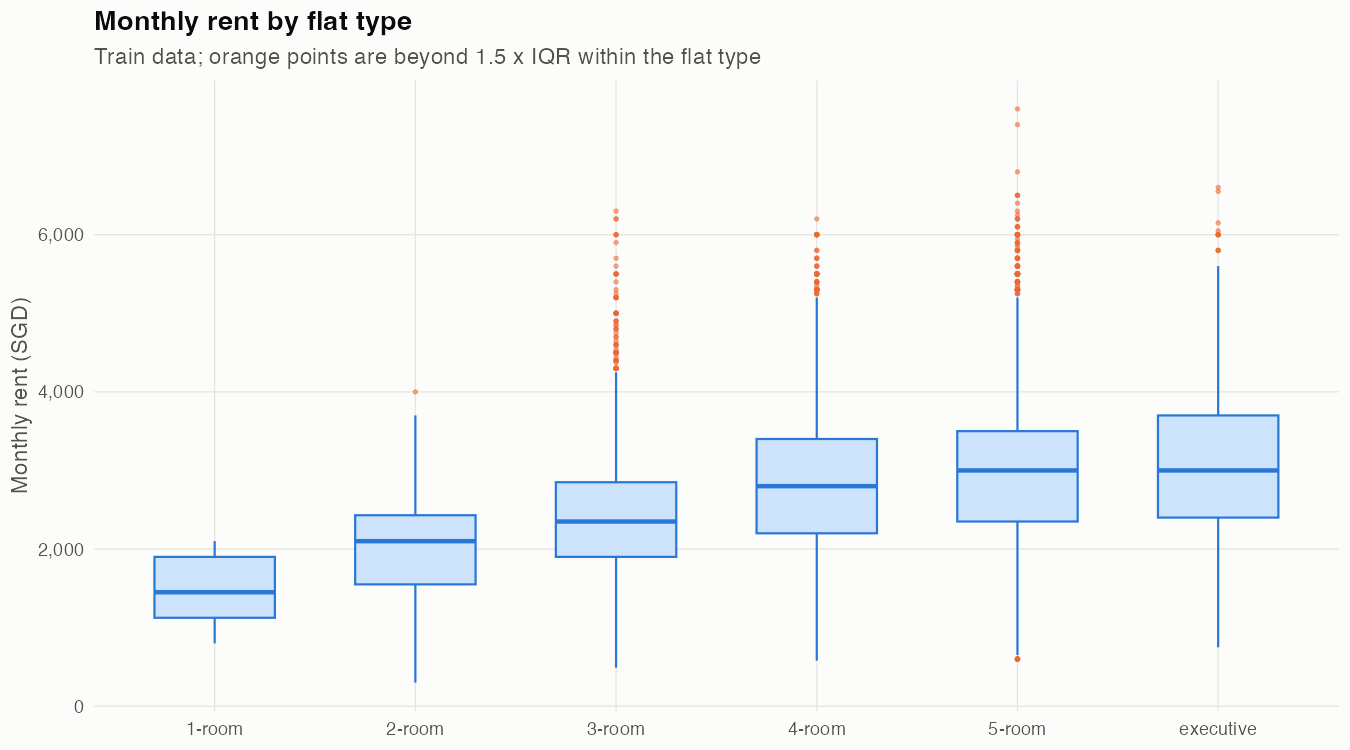
\includegraphics[width=\columnwidth]{../beina/figures/outlier_box_flat_type.png}
\caption{Monthly rent by flat type; points beyond $1.5\times$IQR within the type are shown but kept.\src{Be-out}}\label{fig:box}
\end{figure}

\subsection{Noise floor}
Rows sharing every model input get the same prediction from any deterministic model, so rent spread inside such groups is irreducible. Three groupings give similar estimates: SD 461 for same-unit rentals in one quarter;\src{Be-noise} 464.0 over all labelled months and 454.8 on window P1 for groups sharing all eight inputs;\src{Pu-noise} and 464 for flats in one block, type and month, covering 26.8\% of rows.\src{Aa-noise} Rents are also rounded (87.5\% end in 00), which adds to the noise.\src{Be-round} Our local RMSE of about 450 is of the same order. These estimates cover only rows with a twin and exclude test-period noise.\src{Pu-noise-limit}

\section{Preprocessing and Features}
Table~\ref{tab:eda2prep} traces each exploratory finding to the preprocessing decision it motivated; the pipeline is in Fig.~\ref{fig:flow}.

\begin{table*}[t]
\caption{From exploratory findings to preprocessing decisions.}\label{tab:eda2prep}
\centering\footnotesize
\begin{tabular}{@{}p{5.9cm}p{5.9cm}p{3.6cm}@{}}
\toprule
Finding & Decision & Evidence\\
\midrule
Rent up 53\% then flat; trees cannot extrapolate & Predict the residual over an official median; chronological validation only & Sec.~II-B, Table~\ref{tab:base}\\
COE, stocks and date share only the trend & Drop COE and stocks; never validate on random splits & Sec.~II-C\\
Block-level premiums dominate the residual & Nested shrinkage encodings for block, street and subzone & Table~\ref{tab:imp}\\
Spelling variants (\texttt{STREET} 1,146 to 576 values) & Normalise strings; use native categoricals & Sec.~II-D\\
Sentinel $-1$ values; one bad median entry & Impute from block statistics; remove the entry & Sec.~II-D\\
Outliers are real units and the test set has similar rows & Keep every row; no tail trimming & Sec.~II-D, Table~\ref{tab:matter}\\
Rents rounded; identical flats differ in rent & Treat as a noise floor; do not chase sub-point gains & Sec.~II-E\\
Published medians cover the test quarters & Honest anchor: frozen at 2025-Q1 plus drift & Sec.~III-B, Table~\ref{tab:honest}\\
\bottomrule
\end{tabular}
\end{table*}

\begin{figure*}[t]
\centering
\resizebox{0.98\textwidth}{!}{%
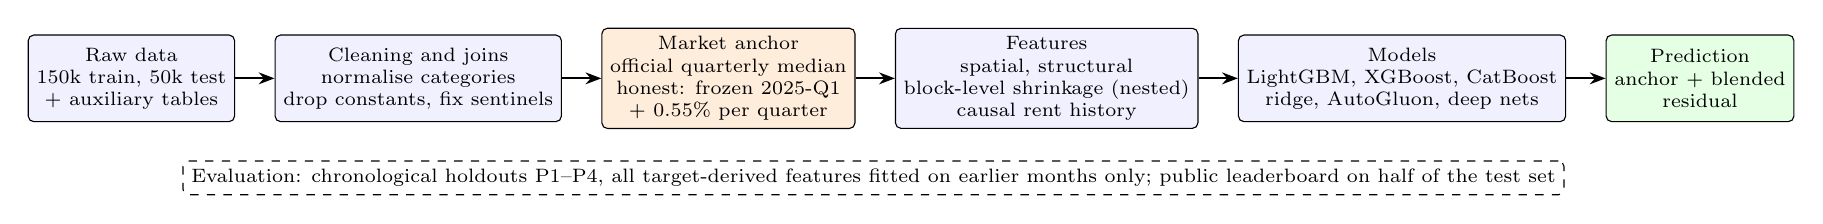
\begin{tikzpicture}[node distance=5mm,
 box/.style={draw,rounded corners=2pt,align=center,minimum height=11mm,font=\scriptsize,fill=blue!6,inner sep=3pt},
 arr/.style={-{Stealth[length=2mm]},thick}]
\node[box] (raw) {Raw data\\150k train, 50k test\\+ auxiliary tables};
\node[box,right=of raw] (clean) {Cleaning and joins\\normalise categories\\drop constants, fix sentinels};
\node[box,right=of clean,fill=orange!14] (anchor) {Market anchor\\official quarterly median\\honest: frozen 2025-Q1\\+ 0.55\% per quarter};
\node[box,right=of anchor] (feat) {Features\\spatial, structural\\block-level shrinkage (nested)\\causal rent history};
\node[box,right=of feat] (model) {Models\\LightGBM, XGBoost, CatBoost\\ridge, AutoGluon, deep nets};
\node[box,right=of model,fill=green!10] (out) {Prediction\\anchor + blended\\residual};
\draw[arr] (raw)--(clean); \draw[arr] (clean)--(anchor); \draw[arr] (anchor)--(feat); \draw[arr] (feat)--(model); \draw[arr] (model)--(out);
\node[draw,dashed,rounded corners=2pt,font=\scriptsize,align=center,below=4mm of feat,xshift=-2.2cm,inner sep=3pt] (ev) {Evaluation: chronological holdouts P1--P4, all target-derived features fitted on earlier months only; public leaderboard on half of the test set};
\end{tikzpicture}}
\caption{Design shared by the four pipelines. The anchor and its honest variant are the central design choice.}\label{fig:flow}
\end{figure*}

\subsection{Cleaning and leakage control}
Rental and block strings are lowercased, trimmed and joined on town, block and street; after normalisation every train and test row matches exactly one block.\src{Be-join} Every target-derived feature for a row in month $t$ uses only labels from months before $t$,\src{Pu-leak} and encoders are fitted inside each training split with inner five-fold out-of-fold values so a row's rent never enters its own feature.\src{Be-te-leak}

\subsection{Market anchor and its honest variant}
The target is rent minus the official median rent for the row's town, flat type and quarter; predictions add it back. Because 51.8\% of the table's values are missing, a fallback chain fills each row: its own cell (96.6\% of train rows), then the national median for the flat type (3.3\%), then adjacent quarters.\src{Be-anchor}

The file runs to 2026-Q2, but a quarter's median aggregates that quarter's rents, so values after the last labelled quarter feed test-period information into the anchor.\src{Be-leak} Our first submission (V2) used them.\src{Aa-v2anchor} The honest variant freezes each cell at 2025-Q1 and multiplies by $\exp(g\,k)$ for $k$ quarters ahead, where $g$ is the mean quarterly log growth of a national index over the last four quarters (+0.55\% at 2025-Q1).\src{Be-drift} Our implementation reproduces the published drift values (+0.78\% at 2024-Q2, +0.55\% at 2025-Q1).\src{Aa-drift}

\subsection{Block-level shrinkage encodings}
High-cardinality keys (14,828 block $\times$ flat-type levels, 576 streets) are encoded by empirical-Bayes shrinkage~\cite{micci}\src{Aa-fp,Me-cat} toward their parent key:
\begin{equation}
\hat\mu_k=\frac{n_k\,\bar r_k+M\,\hat\mu_{\mathrm{parent}(k)}}{n_k+M},\label{eq:te}
\end{equation}
where $\bar r_k$ is the mean residual of key $k$. The hierarchy is town ($M{=}30$), block ($10$), block $\times$ flat type ($5$), street ($15$), subzone ($20$).\src{Aa-M} The R pipeline uses the same constants for the shared levels.\src{Be-te} Hand-set constants proved near-optimal: a random-effects fit recovered 16 for street and 21 for subzone (against 15 and 20) and gave no reliable gain elsewhere.\src{Aa-gpb}

\subsection{Other features}
Structural features (floor area, area per room, maximum floor, year completed, flat age) and distances to the nearest MRT station, mall, school and the CBD with counts within radii\src{Be-spatial} are common to all pipelines. In the V2 pipeline these are computed once per unique block with scikit-learn \texttt{BallTree} indexes under the Haversine metric: nearest distance and counts within 0.5, 1 and 2~km for MRT stations (all, operating, planned, multi-line interchange), malls and primary, secondary and top-tier schools, 20 features in all, including inverse-distance proximity scores.\src{Aa-ball} The R pipeline computes the same kinds of distances independently. The history pipeline adds a 24-month global rent lag and smoothed town $\times$ flat-type and block $\times$ flat-type means with counts; removing the property-level history raises RMSE by 4.388.\src{Pu-hist,Pu-hist-abl} The earlier single-LightGBM root pipeline adds an address-level trailing rent per square metre, which lowers its validation RMSE from 456.70 to 452.56.\src{Aa-addr} The AutoGluon pipeline adds nearest-place names.\src{Me-feat}

\section{Data Mining Methods}
\subsection{Models}
Tabular data with mixed numeric and high-cardinality categorical inputs and 150,000 rows suits boosted trees; trees remain strongest on medium-sized tabular data~\cite{grinsztajn}, and under time-based splits gradient-boosted trees and embedding MLPs rank best~\cite{tabred}. We use LightGBM~\cite{lightgbm}, XGBoost~\cite{xgboost} and CatBoost~\cite{catboost} (ordered target statistics), ridge regression, FT-Transformer~\cite{ftt}, TabTransformer~\cite{tabt}, MLPs, a Temporal Fusion Transformer~\cite{tft} for segment-level forecasts, neural gates and segmented models. The AutoGluon pipeline's AutoGluon-Tabular~\cite{autogluon} setup restricts its base models to LightGBM and CatBoost; AutoGluon's second-level weighted ensemble learns global blend weights, unlike the input-dependent neural gates tested separately, and is extended in later experiments with stacked residual layers. We also reproduced a delayed neural network for Singapore housing prices~\cite{wang2016}.\src{Me-families,Be-paper} Empirical-Bayes target encoding~\cite{micci} and its regularised, cross-fitted forms~\cite{pargent} are standard for high-cardinality keys; random-effects boosting~\cite{gpboost} is the likelihood-based counterpart, which we test in Section~\ref{sec:matter}.

\textbf{Categorical handling.} Categoricals are passed natively to the tree learners; this beat one-hot encoding in six of seven configurations (town, region and block: 481.89 against 482.09),\src{Me-onehot} and replacing every categorical by its target mean was 6.1 to 10.7 RMSE worse.\src{Me-te-all} In the AutoGluon pipeline's selected configuration, automatic text feature generation is disabled with the \texttt{ignore\_text} preset. Thus fields such as street and nearest-MRT name remain categorical, without automatically generated text-special or n-gram columns.\src{Me-text} Encodings of block-like keys are the exception, because they carry information no other feature has (Table~\ref{tab:imp}). Missing numeric block attributes fall back to the town--street median, then the town median, then the global median.\src{Me-fallback}

\subsection{Automated Feature-Selection Experiments}
After establishing a compact manual subset of structurally meaningful property, time, location and accessibility variables, the AutoGluon pipeline evaluated automated selection on a broader 36-variable pool. Two wrapper methods were tested: permutation-importance recursive feature elimination (RFE), which repeatedly refitted the LightGBM--CatBoost ensemble before removing weak variables, and SHAP ranking followed by top-$k$ refits. Chronological rank correlation, mutual information and matched ablations provided supporting diagnostics rather than full-period correlation alone. PCA and truncated SVD were used only as diagnostics because their leading components were not temporally stable. Test labels were never used for selection.\src{Me-fs-manual,Me-fs-auto,Me-dim}

\subsection{Choice of baseline for the residual}
A residual target only helps if the baseline carries the right level. Table~\ref{tab:base} compares baselines across pipelines. A national-level baseline, even an oracle one that knows the actual national average, is worse than the official town $\times$ flat-type median,\src{Be-two-stage} and the history pipeline's residual over a global 24-month lag collapses (CatBoost 662.5 against 464.2 for direct prediction) because the lag lacks town and flat-type detail.\src{Pu-lagres} An explicit trend-plus-residual network is likewise weaker than direct deep prediction (518.6 against 495.9).\src{Me-trendres} Predicting a ratio instead of a difference gave no gain (change $-0.02$).\src{Be-impr}

\begin{table}[t]
\caption{Baselines for the residual target (RMSE).\src{Be-two-stage,Pu-lagres}}\label{tab:base}
\centering\footnotesize
\begin{tabular}{@{}p{4.6cm}p{2.9cm}@{}}
\toprule
Baseline (protocol) & RMSE\\
\midrule
Town $\times$ flat-type official median (P2) & 452.19\\
National level, last 3 months carried forward & 461.99\\
National level, oracle (actual average) & 459.07\\
National level, linear trend & 556.33\\
\midrule
Global 24-month lag, LightGBM / CatBoost (P1): residual & 646.6 / 662.5\\
\hspace{1.2em}same models, direct prediction & 470.8 / 464.2\\
\bottomrule
\end{tabular}
\end{table}

\subsection{Hyperparameters}
The V2 pipeline fixes its settings (LightGBM 1,200 trees, 75 leaves, rate 0.04, early stopping on each fold's validation split).\src{Aa-hp} The R pipeline ran 12, 10 and 6-trial random searches for LightGBM, XGBoost and CatBoost;\src{Be-hp} the history pipeline fixed three LightGBM capacities and three CatBoost seeds and early-stops on the validation window;\src{Pu-hp} the AutoGluon pipeline used 25 trials per model family, supplying the validation period as tuning data.\src{Me-hpo} On the root pipeline a grid, two random searches and a 100-trial Optuna~\cite{optuna} search all fell inside the cross-validation noise: Optuna's best configuration scored 453.71 against 452.56 for the shipped one.\src{Aa-optuna}

\subsection{Blending and final system}
Weights are fitted on out-of-fold or validation predictions: SLSQP in the V2 pipeline (0.545, 0.075, 0.380 for LightGBM, XGBoost, CatBoost),\src{Aa-w} softmax-constrained in the R pipeline,\src{Be-blend} non-negative bounded to $[0,0.85]$ in the history pipeline.\src{Pu-blend}

\textbf{Final models.} We selected two final submissions. The first is five-fold bagged LightGBM, XGBoost and CatBoost on the residual over the \emph{honest} anchor, with the weights above. It scored 433.65480 on the public leaderboard, 0.048 above the version that used published test-quarter medians.\src{Aa-final,Aa-honest-lb} The second is the R pipeline's honest-anchor blend, the version its report adopts; the same setup with COE and stocks scored 433.89670, and the final run without them had not been scored when that report was written.\src{Be-final}

\section{Evaluation and Interpretation}
\subsection{Protocols}
The pipelines used different chronological splits (Table~\ref{tab:proto}); scores compare only within a protocol. Early stopping, candidate selection and blend weights use the validation labels in every pipeline, so local scores are model-selection scores, not untouched estimates; only the leaderboard is independent, and it covers half the test rows.\src{Pu-sel,Me-sel} RMSE is the competition metric; differences are tested with a paired bootstrap that resamples block--month groups (300 draws in the V2 pipeline; 2,000 group resamples in the history pipeline) because rows in one group share unit-level noise.\src{Aa-boot,Pu-noise}

\begin{table}[t]
\caption{Validation protocols.}\label{tab:proto}
\centering\footnotesize
\begin{tabular}{@{}llp{4.6cm}@{}}
\toprule
ID & Pipelines & Fit / validate\\
\midrule
P1 & AutoGluon, history & before 2024-05 (117,988) / 2024-05 to 2025-03 (32,012)\src{Me-split,Pu-W}\\
P2 & V2, R & through 2024-06 (124,016) / 2024-07 to 2025-03 (25,984)\src{Be-split,Aa-e2split}\\
P3 & V2, history (W2) & before 2024-10 (132,802) / 2024-10 to 2025-03 (17,198); the root pipeline drops 641 duplicate rows\src{Pu-W,Aa-dup}\\
P4 & V2 & through 2023-11 / 2023-12 to 2025-03 (16 months)\src{Aa-honest-cost}\\
\bottomrule
\end{tabular}
\end{table}

\subsection{Model comparison}
Table~\ref{tab:results} gives representative results. On P1 the boosted-tree ensemble with causal rent history (463.2) beats AutoGluon without HPO (467.1) by 4 RMSE, and every deep model, gate or router is worse: the best deep expert scores 477.0, TabTransformer 495.9, and segmenting by town or flat type loses 4.6 to 7.6 against the global control.\src{Pu-me,Me-res,Me-seg} On P2 the anchor-and-encoding recipe reaches 450--452 with published medians and 454.9 with the honest anchor, and the R pipeline gives 449.65 and 454.72.\src{Be-res,Aa-honest-cost} On P3, the V2-recipe LightGBM scores 443.64 against 448.688 for the history pipeline's detailed LightGBM, but the first uses published medians and the second none, so the two are not like-for-like.\src{Aa-tab,Pu-w2} A Temporal Fusion Transformer forecasts town $\times$ flat-type monthly means well (RMSE 258.453, $R^2$ 0.8400 on 1,340 segment-months), but adding a listing-level residual model is worse than predicting listings directly (499.791 against 471.209).\src{Me-tft}

\begin{table}[t]
\caption{Representative local RMSE (SGD) by protocol. $^\dagger$published medians; $^\ddagger$honest anchor.\src{Aa-tab,Be-res,Me-res,Pu-me,Pu-w2}}\label{tab:results}
\centering\footnotesize
\begin{tabular}{@{}l@{\hspace{4pt}}l@{\hspace{4pt}}p{3.2cm}r@{}}
\toprule
Prot. & Pipeline & Model & RMSE\\
\midrule
P1 & History & CatBoost, best single seed & 463.549\\
P1 & History & blend v2 / + \sgd/sqm model (v3) & 463.155 / 462.906\\
P1 & AutoGluon & 18 features, no HPO & 467.122\\
P1 & AutoGluon & + one weighted residual layer & 468.057\\
P1 & AutoGluon & deep experts: best / equal blend & 476.979 / 471.168\\
P1 & AutoGluon & TabTransformer & 495.853\\
P2 & R & ridge / LightGBM$^\dagger$ & 451.95 / 452.29\\
P2 & R & XGBoost / CatBoost$^\dagger$ & 450.97 / 450.27\\
P2 & R & blend$^\dagger$ / blend$^\ddagger$ (3 seeds) & 449.65 / 454.72\\
P2 & V2 & CatBoost / LightGBM$^\dagger$ & 450.43 / 452.48\\
P2 & V2 & blend 0.2/0.8$^\dagger$ / blend$^\ddagger$ & 450.30 / 454.85\\
P3 & History & blend v2 / detailed LightGBM & 443.3 / 448.688\\
P3 & V2 & LightGBM$^\dagger$ & 443.64\\
\bottomrule
\end{tabular}
\end{table}

\subsection{Automated Feature-Selection Results}
The controlled manual screen selected a compact 13-variable subset at RMSE 467.230, ahead of the 31-variable full table at 467.507 and the 25-variable candidate expansion at 468.304. The selected production representation subsequently extended the compact set with a prior-only town $\times$ flat-type mean, a global 24-month rent lag and three nearest-place names; its default LightGBM--CatBoost ensemble scored 467.122. Because training budgets and automatic text handling differed between these stages, the latter comparison is a development progression rather than a pure one-variable ablation.\src{Me-fs-manual}

Automated reduction did not establish a stronger independent result. RFE retained all 36 candidates at 468.921; reducing to 10 produced 469.080, while intermediate subsets were less stable. Under the same shortened protocol, the SHAP top-18 subset scored 467.841 against 468.272 for the manual 18-variable set. This 0.431 improvement was selected on the same outer validation period, so it was not treated as an untouched estimate and did not replace the production representation. PCA showed the same temporal-instability warning: the first numeric component's target correlation fell from 0.654 in fitting to 0.306 in validation, and no PCA/SVD replacement-model RMSE was recorded.\src{Me-fs-auto,Me-dim}

\begin{table}[t]
\caption{Automated Feature-selection results on P1.\src{Me-fs-manual,Me-fs-auto}}\label{tab:feature-selection}
\centering\footnotesize
\begin{tabular}{@{}p{2.0cm}p{3.9cm}r@{}}
\toprule
Method & Selected / matched comparator & RMSE\\
\midrule
Manual subsets & Compact 13 / full 31 & 467.230 / 467.507\\
RFE & All 36 / reduced 10 & 468.921 / 469.080\\
SHAP top-$k$ & Top 18 / manual 18 & 467.841 / 468.272\\
\bottomrule
\end{tabular}
\end{table}

\subsection{Alternative Modelling Approaches}
Table~\ref{tab:alternatives} compares the principal alternatives evaluated in the AutoGluon pipeline on the common P1 listing holdout.
Hard segmentation did not help: routing AutoGluon by town and flat type scored 475.846 and 476.068, against global controls of 468.272 and 471.448.
The same pattern held for random forests: the global model scored 484.923, flat-type routing scored 486.073, and chronological tuning improved the global forest to 479.319 but left it well behind boosted trees.
Splitting the data therefore lost more shared signal than it gained from local specialisation.\src{Me-seg,Me-alt}

Deep tabular models learned useful structure but remained weaker than tree ensembles. The best individual deep expert, 
an FT-Transformer, scored 476.979; TabTransformer scored 495.853, while averaging three deep experts improved to 471.168. 
A block-to-town neural gate scored 475.130, so input-dependent routing was again inferior to a fixed blend. The standalone FT-Transformer run scored 497.497, 
and an explicit neural trend-plus-residual decomposition scored 518.590.\src{Me-res,Me-trendres,Me-alt}

Asymmetric and residual-specialist models also showed the value of shrinkage. Quantile LightGBM at $q{=}0.60$ reduced MAE from 356.438 to 343.087 
and shifted predictions toward over-forecasting, but worsened RMSE from 478.370 to 492.281. Weighted flat-type residual experts 
made a small improvement over their matched Layer-1 control (468.272 to 468.068); the significant-residual gate scored 468.360 and the unweighted segmented correction 
deteriorated to 472.509. Thus residual models helped only when their corrections were strongly attenuated.\src{Me-alt}

Time-series experiments used different targets or holdouts and are not included in Table~\ref{tab:alternatives}. A property-group time-series ensemble scored 477.592 
on observed item-months. A town $\times$ flat-type market forecast reached 273.240 at segment level, but its listing hybrid scored 486.052. Likewise, TFT reached 258.453 on segment-month means, 
yet TFT plus a listing residual scored 499.791 against 471.209 for direct listing prediction. Under rolling-origin evaluation, an explicit trend-plus-residual model scored 571.673 against 567.562 for the direct baseline. 
Aggregate temporal patterns were learnable, but their errors compounded when forecasts were translated back to individual listings.\src{Me-tft,Me-alt}

\begin{table}[t]
\caption{Alternative listing-level models evaluated using validation RMSE under the P1 protocol.\src{Me-res,Me-seg,Me-alt}}\label{tab:alternatives}
\centering\scriptsize
\begin{tabular}{@{}p{1.45cm}p{5.05cm}r@{}}
\toprule
Approach & Model description & P1 RMSE\\
\midrule
Reference & AutoGluon LightGBM--CatBoost, default settings & \textbf{467.122}\\
Residual specialists & Weighted flat-type residual experts & 468.068\\
 & Significant-residual gated specialist & 468.360\\
Fixed / learned blends & Equal LightGBM--CatBoost blend & 468.740\\
 & Equal deep-expert blend & 471.168\\
 & Neural LightGBM--CatBoost gate & 472.274\\
 & Block-to-town deep gate & 475.130\\
Hard segmentation & Town-routed AutoGluon & 475.846\\
 & Flat-type-routed AutoGluon & 476.068\\
Random forests & Chronologically tuned random forest & 479.319\\
 & Global random forest & 484.923\\
 & Flat-type-routed random forest & 486.073\\
Asymmetric loss & Quantile LightGBM ($q{=}0.60$) & 492.281\\
Deep tabular & TabTransformer & 495.853\\
 & FT-Transformer & 497.497\\
\bottomrule
\end{tabular}
\end{table}

\subsection{What mattered and what did not}\label{sec:matter}
Table~\ref{tab:matter} separates the changes that moved the score from those that did not. The anchor is decisive over a long horizon: on P4 it cuts RMSE from 600.72 to 492.77, while on a 6-month window the gain is not significant.\src{Aa-anchor} Target encodings, mostly at block level, are the other component that matters: removing all seven costs 8.68 RMSE for the blend and 19.47 for ridge,\src{Be-te-abl} and the step from V1 to V2, which added hierarchical encodings (and interchange-distance features), is the only visible jump on the leaderboard (Fig.~\ref{fig:lb}).\src{Aa-lb} Almost everything else lies within about one RMSE or is worse. Tuning moves results by under 1.2 in the R pipeline's experiments, and recency weighting is reliably worse because it discards block information.\src{Be-impr} Table~\ref{tab:imp} shows where the signal sits: the encodings dominate, the benchmark features come next, and COE and stocks contribute nothing.

\begin{table}[t]
\caption{Permutation importance by feature group: increase in out-of-time RMSE when shuffled (CatBoost, R pipeline).}\label{tab:imp}
\centering\footnotesize
\begin{tabular}{@{}lr@{\hspace{1.4em}}lr@{}}
\toprule
Group & $\Delta$ & Group & $\Delta$\\
\midrule
All 7 encodings & +40.4 & Flat model & +2.1\\
Location encodings & +34.2 & MRT & +1.4\\
Benchmark features & +13.1 & Time & +0.1\\
Flat age, lease year & +6.2 & Stocks & $-0.06$\\
CBD distance & +5.7 & COE & $-0.08$\\
\bottomrule
\end{tabular}\src{Be-imp}
\end{table}

\begin{table*}[t]
\caption{Effect of changes on RMSE (positive = worse). CI = paired-bootstrap 95\% interval; n.s. = not significant.}\label{tab:matter}
\centering\footnotesize
\begin{tabular}{@{}p{5.8cm}p{5.6cm}p{4.0cm}@{}}
\toprule
Change & Effect & Where measured\\
\midrule
Residual over anchor, long horizon & 600.72 $\to$ 492.77\src{Aa-anchor} & P4, root pipeline\\
Residual over anchor, 6-month window & 452.56 $\to$ 451.87 (CI $-1.98$ to $+0.52$, n.s.)\src{Aa-anchor} & P3, root pipeline\\
Target encodings removed (7 keys, mostly block-level) & +8.68 blend, +19.47 ridge\src{Be-te-abl} & P2 (R)\\
Property-level rent history removed & +4.388\src{Pu-hist-abl} & P1 (history)\\
Address-level trailing feature added & $-4.14$ (456.70 $\to$ 452.56)\src{Aa-addr} & P3, root pipeline\\
\midrule
Optuna, 100 trials, vs shipped configuration & +1.15 (453.71 vs 452.56)\src{Aa-optuna} & P3, root pipeline\\
Huber, Fair, L1 losses (Huber $\delta{=}1000$ ties) & +0.7 to +4.9\src{Aa-robust} & P2, P4\\
Trimming 0.5--2.5\% from each tail & +1.7 to +10.6\src{Aa-trim} & P2, P4\\
Random-effects model (GPBoost) replacing encodings & +5.26 and +7.98\src{Aa-gpb} & P2, P4\\
External resale premium by block / neighbour-block priors & $-0.56$, $-0.15$ (n.s.) / $-0.25$ (n.s.), +0.82\src{Aa-resale} & P2, P4\\
Neural gate vs equal blend; town / flat-type routing & +3.5; +7.6 / +4.6\src{Me-res,Me-seg} & P1 (AutoGluon)\\
Prediction-as-feature second layer; AdaBoost residual & +69.9; +29.1\src{Me-stack} & P1 (AutoGluon)\\
Recency weighting (24-month half-life) & +1.14\src{Be-impr} & P2 (R)\\
CatBoost-heavy blend weights & $-0.51$ / $-1.09$ locally, public score +0.023\src{Aa-cbw,Aa-lb} & P2, P4; leaderboard\\
Honest instead of published anchor & +4.55 (P2), public score +0.048\src{Aa-honest-cost,Aa-honest-lb} & P2; leaderboard\\
\bottomrule
\end{tabular}
\end{table*}

\subsection{Local gains against the leaderboard}
Fig.~\ref{fig:lb} shows every submission. The anchor-and-encoding pipelines, the causal-history pipeline and the AutoGluon LightGBM--CatBoost stack fall within 433.4 to 436.3, a plateau only 0.7\% wide. Three local gains of 0.5 to 3 RMSE (deeper trees, premium and bagging, CatBoost-heavy weights) did not appear on the leaderboard (434.05, 434.03, 433.63 against V2's 433.61),\src{Aa-lb,Aa-cbw,Aa-trim} consistent with the public score covering half the test rows and unit-level noise dominating.\src{Pu-lb-limit} Published studies find public leaderboards rank reliably despite adaptive reuse~\cite{roelofs} but that tiny differences carry little information~\cite{ladder}.

\begin{figure}[t]
\centering
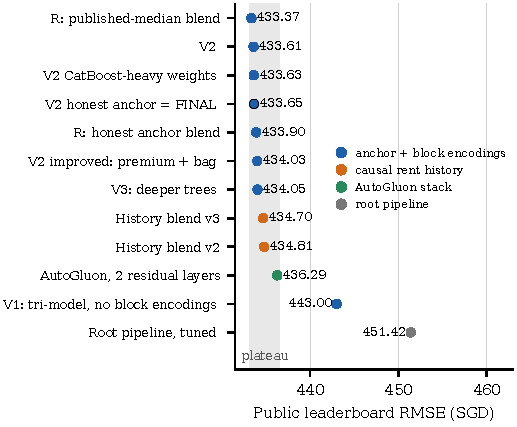
\includegraphics[width=\columnwidth]{figures/fig_leaderboard.pdf}
\caption{Public leaderboard RMSE of every submission by pipeline. The final model is outlined.\src{Aa-lb,Be-lb,Pu-lb,Me-lb}}\label{fig:lb}
\end{figure}

\subsection{Honest anchor}
Table~\ref{tab:honest} quantifies the cost of removing test-period information on the V2 recipe. On P2 it is 4.6 to 6.3 RMSE, matching the R pipeline's measurement of about 5 locally and 0.5 on the leaderboard.\src{Aa-honest-cost,Be-honest-lb} Drift helps when the market is flat (mean error falls from +47.6 to +1.8) but is catastrophic after a surge: at the 2023-Q3 cutoff $g$ was +5.05\% per quarter and extrapolating it over six quarters over-predicted by 885 by 2025-Q1. At the true cutoff $g$ is only +0.55\%, the flat case. The same fragility appears in the history pipeline's backtests, where projected market indices help in one regime and hurt in another.\src{Pu-backtest}

\begin{table}[t]
\caption{Anchor variants, blend 0.2 LightGBM / 0.8 CatBoost (RMSE).\src{Aa-honest-cost}}\label{tab:honest}
\centering\footnotesize
\begin{tabular}{@{}lccc@{}}
\toprule
Holdout & Published & Frozen & Frozen + drift\\
\midrule
P2 ($g{=}{+}0.78\%$) & 450.30 & 456.57 & 454.85\\
P4 ($g{=}{+}5.05\%$) & 482.53 & 487.48 & 764.71\\
\bottomrule
\end{tabular}
\end{table}

\subsection{Data volume and recency}
More real data helps much more than tuning: RMSE falls by roughly 6 to 8 per doubling of training rows (465.77 at 13k rows to 443.64 at 133k) with no sign of saturation, and training that ends 9, 12 or 15 months earlier costs 0.92, 1.84 and 4.17 against a same-size recent sample (Fig.~\ref{fig:learn}).\src{Aa-learn} Block premiums are estimated from few transactions (about 8 rows per block-type level), which is the likely reason for the appetite for data. This also explains why synthetic rows cannot help: the gain comes from real transactions at specific blocks.

\begin{figure}[t]
\centering
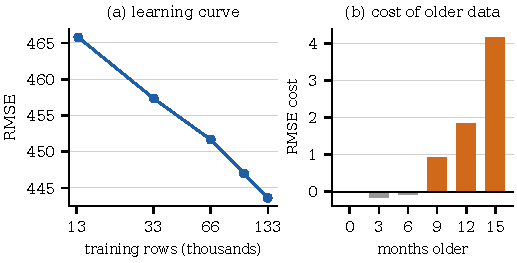
\includegraphics[width=\columnwidth]{figures/fig_learning.pdf}
\caption{(a) RMSE against training rows for V2's recipe on the 2024-10 to 2025-03 window; (b) cost of training data that ends earlier, against a same-size sample.\src{Aa-learn}}\label{fig:learn}
\end{figure}

\subsection{Where the model fails}
Error is concentrated (Fig.~\ref{fig:resid}). On the root pipeline the 6.5\% of validation rows with rent at or below \sgd 2,100 have RMSE 1,090 against 370 for the rest, and so carry 37.5\% of the squared error.\src{Aa-tail} The AutoGluon pipeline's out-of-fold diagnostics show the same pattern by segment: executive flats have RMSE 720, five-room 653 and three-room 542.\src{Me-seg-err} Within a block, flat type and month, rents differ with SD 464, so most of this is not recoverable from the available columns.\src{Aa-noise} The history pipeline finds that on rows with an exact twin, RMSE (452.8) lies inside the interval for the noise estimate (442.2 to 466.8), and that rows without a twin score 14.1 worse, which noise and headroom cannot separate.\src{Pu-twin} Table~\ref{tab:backtest} shows the level error in a rising market. A model that ignores the market also lags: in a rising-market backtest the history pipeline under-predicts by 312 on average, and supplying the true index cuts RMSE from 629.9 to 500.2.\src{Pu-backtest}

\begin{table}[t]
\caption{Moving-market backtests of the history pipeline: 12-month windows after each origin, LightGBM fitted on all earlier rows. Bias is prediction minus actual; the oracle index deflates the target by a market index that includes the validation months.}\label{tab:backtest}
\centering\footnotesize
\begin{tabular}{@{}lccc@{}}
\toprule
Origin & 2022-01 & 2023-01 & 2024-01\\
\midrule
Rent change & +30.0\% & +5.5\% & +2.0\%\\
Control RMSE & 629.9 & 629.1 & 493.9\\
Control bias & $-312.2$ & $-152.0$ & +14.2\\
Oracle RMSE & 500.2 & 604.6 & 490.6\\
Noise SD & 471.3 & 588.5 & 479.3\\
\bottomrule
\end{tabular}\src{Pu-backtest}
\end{table}

\begin{figure}[t]
\centering
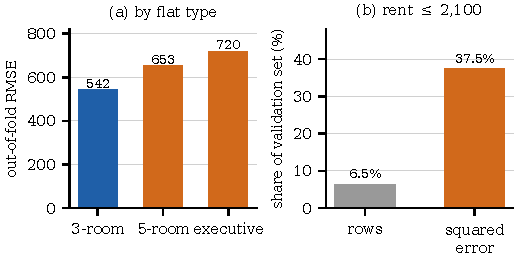
\includegraphics[width=\columnwidth]{figures/fig_errors.pdf}
\caption{Where the error sits: (a) out-of-fold RMSE by flat type (AutoGluon pipeline); (b) the 6.5\% of validation rows with rent at or below \sgd 2,100 carry 37.5\% of the squared error (root pipeline).\src{Me-seg-err,Aa-tail}}\label{fig:resid}
\end{figure}

\textbf{Answers to the research questions.} \textbf{Q1:} the official town $\times$ flat-type median as a residual baseline, with block-level shrinkage encodings, carries the level: public RMSE 443.0 to 433.6 and, over a 16-month holdout, 600.72 to 492.77.\src{Aa-lb,Aa-anchor} \textbf{Q2:} almost nothing else adds more than about one RMSE (Table~\ref{tab:matter}), although more real data does help (Fig.~\ref{fig:learn}). \textbf{Q3:} identical flats differ with SD 455--464 against our local RMSE of about 450, so little headroom remains.\src{Pu-noise,Aa-noise} \textbf{Q4:} local gains of 0.5 to 3 did not reach the leaderboard, and the honest anchor costs 4.6 locally but 0.05 publicly, so local protocols both over- and under-state differences; paired intervals and the leaderboard should be read together.\src{Aa-lb,Aa-honest-cost,Aa-honest-lb}

\section{Limitations and Future Work}
\textbf{Evaluation.} Every local score reuses validation labels for selection;\src{Pu-sel} protocols differ across pipelines; and the test-period market level is unmeasured, since the history pipeline's leaderboard shift probe was never scored.\src{Pu-probe} \textbf{Anchor.} The published medians leak test-period aggregates; our honest variant costs little on the leaderboard but its drift rule is regime-dependent. \textbf{Information.} No dataset we could use legitimately separates units within a block: the official rental registry carries the same fields as ours and the target itself, which is why we did not use it, and block-level data cannot tell two flats in one block apart.\cite{hdbrent} Resale-derived signals and neighbour-block priors gave under one RMSE.\src{Aa-resale} \textbf{Future work:} unit-level data (floor, condition) if the course permits it, regime-aware drift selection, recency-aware encodings, and uncertainty estimates for the heavy low-rent tail.

\textbf{Conclusion.} Carrying the market level through an official median anchor and shrinking block-level premiums toward their parents account for the only large gain we found; everything built on top sits inside a noise floor of about 455--464 SGD that our three groupings measure consistently. The honest forecast-time version of the same model scores 433.65480.

\begin{thebibliography}{99}
\bibitem{hdbrent} Housing and Development Board, ``Renting out of flats,'' data.gov.sg, \url{https://data.gov.sg/dataset/renting-out-of-flats}, accessed Oct. 2026.
\bibitem{grinsztajn} L. Grinsztajn, E. Oyallon and G. Varoquaux, ``Why do tree-based models still outperform deep learning on typical tabular data?'' in \emph{Proc. NeurIPS}, 2022.
\bibitem{tabred} I. Rubachev \emph{et al.}, ``TabReD: Analyzing pitfalls and filling the gaps in tabular deep learning benchmarks,'' in \emph{Proc. ICLR}, 2025.
\bibitem{lightgbm} G. Ke \emph{et al.}, ``LightGBM: A highly efficient gradient boosting decision tree,'' in \emph{Proc. NeurIPS}, 2017.
\bibitem{xgboost} T. Chen and C. Guestrin, ``XGBoost: A scalable tree boosting system,'' in \emph{Proc. KDD}, 2016.
\bibitem{catboost} L. Prokhorenkova \emph{et al.}, ``CatBoost: Unbiased boosting with categorical features,'' in \emph{Proc. NeurIPS}, 2018.
\bibitem{autogluon} N. Erickson \emph{et al.}, ``AutoGluon-Tabular: Robust and accurate AutoML for structured data,'' arXiv:2003.06505, 2020.
\bibitem{ftt} Y. Gorishniy, I. Rubachev, V. Khrulkov and A. Babenko, ``Revisiting deep learning models for tabular data,'' in \emph{Proc. NeurIPS}, 2021.
\bibitem{tabt} X. Huang, A. Khetan, M. Cvitkovic and Z. Karnin, ``TabTransformer: Tabular data modeling using contextual embeddings,'' arXiv:2012.06678, 2020.
\bibitem{tft} B. Lim, S. {\"O}. Ar{\i}k, N. Loeff and T. Pfister, ``Temporal fusion transformers for interpretable multi-horizon time series forecasting,'' \emph{Int. J. Forecasting}, vol. 37, no. 4, pp. 1748--1764, 2021.
\bibitem{wang2016} L. Wang, F. F. Chan, Y. Wang and Q. Chang, ``Predicting public housing prices using delayed neural networks,'' in \emph{Proc. IEEE TENCON}, 2016, pp. 3589--3592.
\bibitem{micci} D. Micci-Barreca, ``A preprocessing scheme for high-cardinality categorical attributes in classification and prediction problems,'' \emph{ACM SIGKDD Explor.}, vol. 3, no. 1, pp. 27--32, 2001.
\bibitem{optuna} T. Akiba, S. Sano, T. Yanase, T. Ohta and M. Koyama, ``Optuna: A next-generation hyperparameter optimization framework,'' in \emph{Proc. KDD}, 2019.
\bibitem{pargent} F. Pargent, F. Pfisterer, J. Thomas and B. Bischl, ``Regularized target encoding outperforms traditional methods in supervised machine learning with high cardinality features,'' \emph{Computational Statistics}, 2022, arXiv:2104.00629.
\bibitem{gpboost} F. Sigrist, ``Gaussian process boosting,'' \emph{J. Mach. Learn. Res.}, vol. 23, no. 232, pp. 1--46, 2022.
\bibitem{roelofs} R. Roelofs \emph{et al.}, ``A meta-analysis of overfitting in machine learning,'' in \emph{Proc. NeurIPS}, 2019.
\bibitem{ladder} A. Blum and M. Hardt, ``The Ladder: A reliable leaderboard for machine learning competitions,'' in \emph{Proc. ICML}, 2015.
\end{thebibliography}

\clearpage
\appendices
\section{Workload}\label{app:work}
\begin{table}[h]
\centering\footnotesize
\begin{tabular}{@{}lp{6.0cm}@{}}
\toprule
Member & Main responsibility\\
\midrule
Aayush & Root pipeline and data-quality audit; median-rent residual anchor and its honest forecast-time variant; V2 recipe (hierarchical shrinkage encodings, BallTree spatial features, three-model blend) and leaderboard series; final submission and the end-to-end reproducible \texttt{main.py}; ablations (tail trimming, robust losses, GPBoost, resale, learning curve)\\
Metul & Shared preprocessing; association, mutual-information and PCA analysis; AutoGluon, deep tabular, gating, segmentation, time-series and residual-stack experiments\\
Punyaa & Leakage-safe causal rent-history features; LightGBM/CatBoost ensemble and 76 unit tests; extrapolation, noise-floor and moving-market backtests\\
Beina & R cleaning and EDA; in-fold hierarchical encodings; honest-anchor drift; ablations and feature importance; the second selected final submission (\texttt{predict\_test.R})\\
\bottomrule
\end{tabular}
\end{table}
\emph{This table summarises the content of each member's folder under \texttt{report/}; each member should confirm it.}\src{Wk-P,Wk-M,Wk-B}

\section{Hyperparameters and reproduction}
V2: LightGBM 1,200 trees, 75 leaves, learning rate 0.04, subsample 0.8, column sample 0.75; XGBoost depth 7; CatBoost 1,200 iterations, depth 7, learning rate 0.05; early stopping 40 rounds; five folds, seed 42.\src{Aa-v2hp} The final model is reproduced end to end, from the raw files to \url{submission.csv}, by \url{main.py} with the code in \url{modules/}.\src{Aa-main} Experiment scripts: \url{expt-2/src/models_v2.py} (V2), \url{expt-5/src/honest_v2_submission.py} (honest anchor), \url{expt-5/src/exp6_honest_anchor_validation.py} (Table~\ref{tab:honest}). History pipeline: \url{python3 -m punyaa.train}; R pipeline: \url{model_training.R}, \url{predict_test.R}; AutoGluon pipeline: notebooks under \url{exploration/metul}.\src{Pu-repro,Be-scripts,Me-trace}

\end{document}
"  to show them, plain  pdflatex main  hides them ----
\newif\ifshowsrc
\ifdefined\SHOWSRC\showsrctrue\else\showsrcfalse\fi
\newcommand{\src}[1]{\ifshowsrc\textsuperscript{\tiny\color{gray}[#1]}\fi}

\newcommand{\sgd}{S\$}
\def\BibTeX{{\rm B\kern-.05em{\sc i\kern-.025em b}\kern-.08em T\kern-.1667em\lower.7ex\hbox{E}\kern-.125emX}}

\begin{document}
\pagestyle{plain}
\pagenumbering{arabic}

\title{Forecasting HDB Rents Sixteen Months Ahead:\\Market Anchors, Block-Level Shrinkage and the Noise Floor\\[2pt]\large Team 2 --- [TEAM NAME]}

\author{\IEEEauthorblockN{Aayush Majumdar}
\IEEEauthorblockA{\textit{Student ID A0352046L}\\
\textit{National University of Singapore}}
\and
\IEEEauthorblockN{Metul Prabhu}
\IEEEauthorblockA{\textit{Student ID A0352394Y}\\
\textit{National University of Singapore}}
\and
\IEEEauthorblockN{Punyaa [Surname]}
\IEEEauthorblockA{\textit{Student ID [ID]}\\
\textit{National University of Singapore}}
\and
\IEEEauthorblockN{Beina [Surname]}
\IEEEauthorblockA{\textit{Student ID [ID]}\\
\textit{National University of Singapore}}}

\maketitle
\thispagestyle{plain}

\begin{abstract}
We forecast the monthly rent of 50,000 Singapore HDB flat rentals approved up to sixteen months after our 150,000 labelled examples (2021--2025). We built four pipelines on the same data: gradient-boosted trees on the residual over an official median rent with block-level shrinkage encodings, causal rent-history features, AutoGluon LightGBM--CatBoost stacks plus deep tabular models, and an R pipeline with the first design. Three findings emerge. First, predicting the residual over the official median rent, with block-level encodings, is the only change that moved the public leaderboard materially (443.0 to 433.6 RMSE). Second, deep models, gating, segmentation, hyperparameter search, robust losses, tail trimming and external resale data each moved RMSE by about one point or made it worse. Third, identical flats rent with a standard deviation of about 455--464 SGD, the same order as our error. The released median-rent file covers the test quarters and so leaks future aggregates; an honest forecast-time anchor costs about 5 RMSE locally but 0.05 on the leaderboard. Our final model scores 433.65480.\src{Aa-lb,Aa-honest-lb,Aa-honest-cost,Be-noise,Pu-noise,Aa-noise,Me-families}
\end{abstract}

\section{Introduction}
Rents of public housing are a visible measure of living costs, and the Housing and Development Board (HDB) publishes every approved flat rental as open data~\cite{hdbrent}. A model that predicts a flat's rent helps tenants and owners judge asking rents and helps analysts follow the market. We predict the monthly rent of 50,000 rental approvals dated March 2025 to July 2026 from 150,000 labelled approvals dated January 2021 to March 2025, plus auxiliary tables on blocks, MRT stations, malls, schools, COE premiums, stock prices and official median rents.\src{Pu-task,Be-inputs}

Three properties make the task hard. (i) The test months lie up to sixteen months after the last label,\src{Pu-future} while rents rose 53\% over the labelled period and then flattened.\src{Be-trend} (ii) Location carries most of the signal at a finer grain than any single numeric feature.\src{Be-weakcorr} (iii) Flats that look identical in the data rent for different amounts.\src{Pu-noise}

We ask four questions. \textbf{Q1:} what information lets a model carry the market level to unseen months? \textbf{Q2:} how much can better models add on top? \textbf{Q3:} how much of the error is irreducible? \textbf{Q4:} how far can local validation be trusted against an external leaderboard? We call the four pipelines V2 (boosted trees on the residual over the official median), R (the same design in R), history (causal rent-history features) and AutoGluon (stacks and deep tabular models).

\section{Data and Exploratory Analysis}
\subsection{Data}
Table~\ref{tab:data} lists the inputs. Only eight raw columns vary (approval month, town, block, street, flat type, flat model, floor area, lease start); \texttt{FURNISHED} and \texttt{FEE} are constant and are dropped.\src{Pu-task}

\begin{table}[t]
\caption{Data used.}\label{tab:data}
\centering\footnotesize
\begin{tabular}{@{}p{2.3cm}p{5.2cm}@{}}
\toprule
File & Content\\
\midrule
train / test & 150,000 rentals (2021-01 to 2025-03) / 50,000 (2025-03 to 2026-07)\src{Be-inputs}\\
HDB blocks & 9,464 blocks: coordinates, maximum floor, year completed, subzone\src{Be-inputs}\\
MRT, malls, schools & 243 stations, 113 malls, 337 schools\src{Be-inputs}\\
COE, stocks & monthly premiums, daily prices (tested, not retained)\\
Median rent & 13,305 quarterly values by town and flat type, 51.8\% missing\src{Be-anchor}\\
\bottomrule
\end{tabular}
\end{table}

\subsection{Market drift}
Mean rent rose 53\%, from \sgd 2,055 (first three months) to \sgd 3,142 (last three), nearly all of it between mid-2021 and mid-2023; it has been almost flat since.\src{Be-trend} The official town $\times$ flat-type median follows the level closely (Fig.~\ref{fig:trend}). Trees cannot extrapolate a trend,\src{Pu-trees} so every strong model here predicts the residual over this benchmark instead of rent itself.

\begin{figure}[t]
\centering
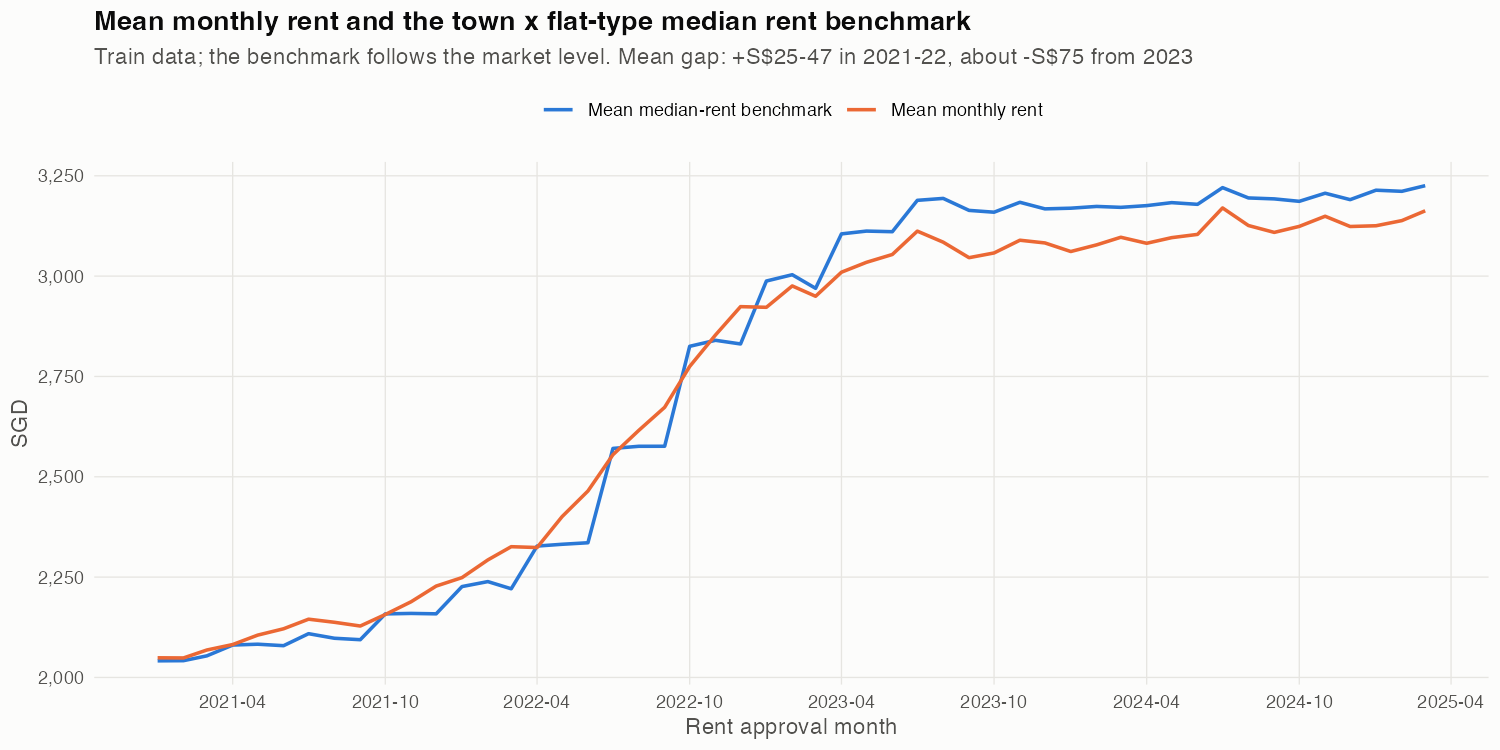
\includegraphics[width=\columnwidth]{../beina/figures/trend_rent_vs_benchmark.png}
\caption{Mean monthly rent and the mean town $\times$ flat-type median benchmark (train months).\src{Be-trend}}\label{fig:trend}
\end{figure}

\subsection{Calendar and macro proxies}
Approval date, COE premium and stock prices correlate strongly with rent over the whole period only because they share the trend. COE correlates 0.898 with monthly mean rent in levels but 0.015 in month-on-month changes.\src{Be-coe} Inside the validation period their rank correlation with rent collapses (COE 0.528 to 0.006, approval date 0.562 to 0.018), whereas the town $\times$ flat-type historical mean keeps 0.664 to 0.668 (Fig.~\ref{fig:assoc}).\src{Me-assoc} Mutual information with rent likewise ranks that historical mean first (0.361), ahead of approval date (0.229) and COE premium (0.218).\src{Me-mi} COE and stocks have negative permutation importance ($-0.08$, $-0.06$) and are dropped.\src{Be-imp} A random split would hide this failure, so all validation is chronological.

\begin{figure}[t]
\centering
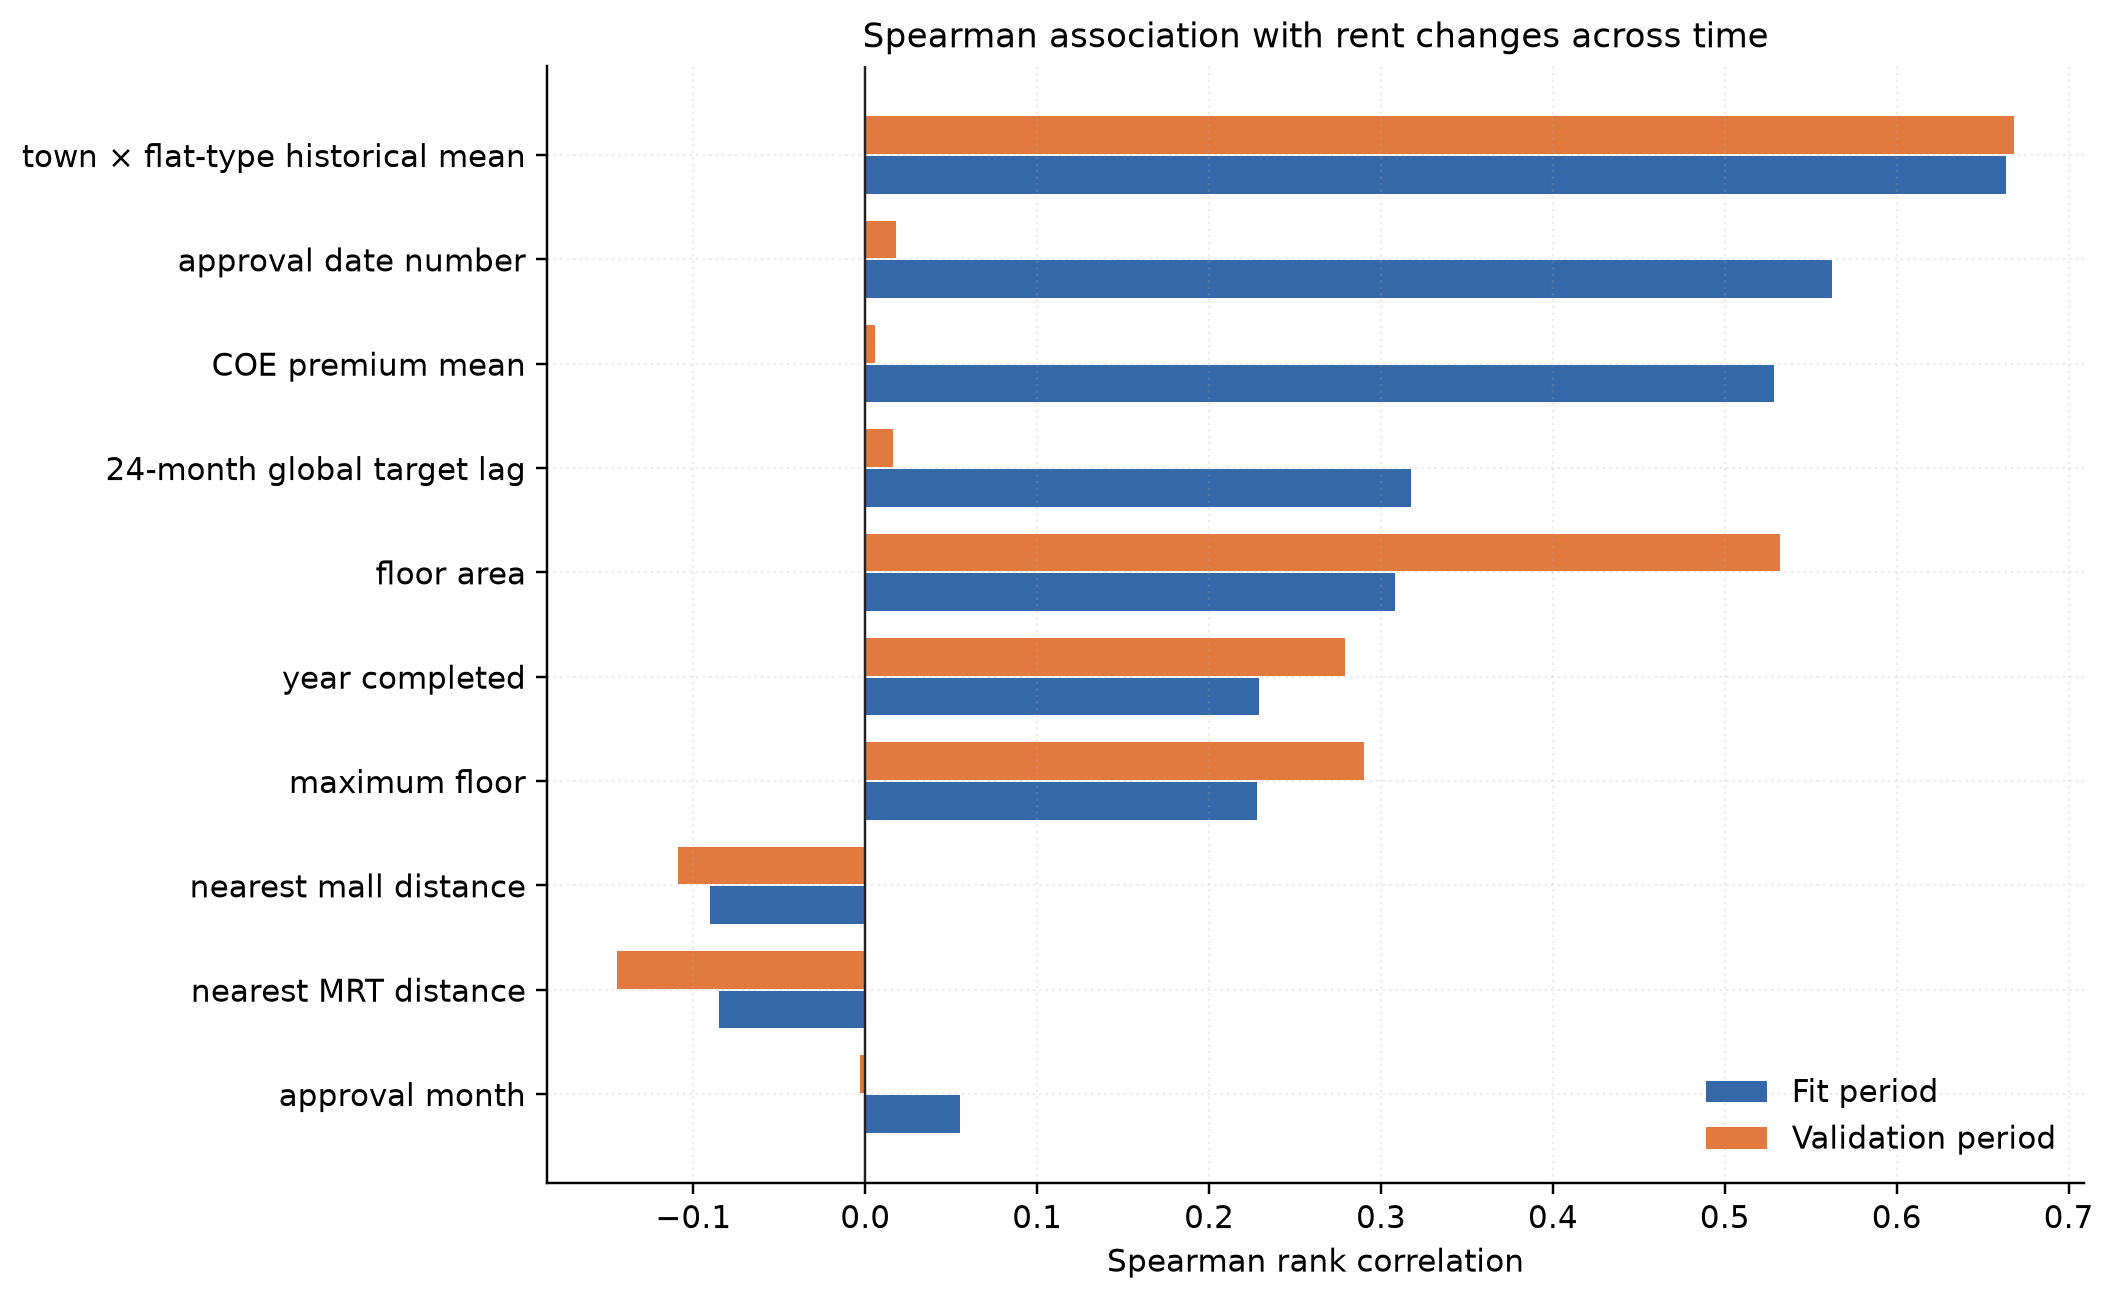
\includegraphics[width=\columnwidth]{../metul/figures/association_stability.png}
\caption{Spearman correlation with rent in the fitting and chronological validation periods (P1 protocol).\src{Me-assoc}}\label{fig:assoc}
\end{figure}

\subsection{Location, categories and outliers}
Once the benchmark is removed the numeric features correlate weakly with the residual ($|r|\le 0.12$), so the remainder is mostly block-level.\src{Be-weakcorr} Shuffling the seven target encodings (mostly block-level) raises out-of-time RMSE by 40.4, the largest effect of any feature group; the four location encodings alone account for 34.2.\src{Be-imp}

Lowercasing and normalising separators cuts \texttt{STREET} from 1,146 to 576 values and \texttt{FLAT\_TYPE} from 11 to 6.\src{Me-cat} Every test town, street, flat type and model occurs in training; 11 unseen block labels affect 36 of 50,000 test rows (0.072\%).\src{Me-cov} Without normalising address casing, 30,781 train rows (20.5\%) fail to join to the block table.\src{Be-join} Eleven blocks store $-1$ for maximum floor and year completed (159 train rows) and are imputed; one median entry (300 against about 3,000 elsewhere) is removed.\src{Be-sent,Be-bad}

We keep every row. The IQR rule flags 130 floor areas and 752 rents,\src{Me-out} but only 0.11\% of rows are extreme relative to their benchmark. The highest rents are real adjoined flats and premium maisonettes, the lowest (\sgd 300--450) are 2-room flats that are probably subsidised or room rentals.\src{Be-out} Removing training tails also hurt RMSE at every level we tried (Section~\ref{sec:matter}).

\begin{figure}[t]
\centering
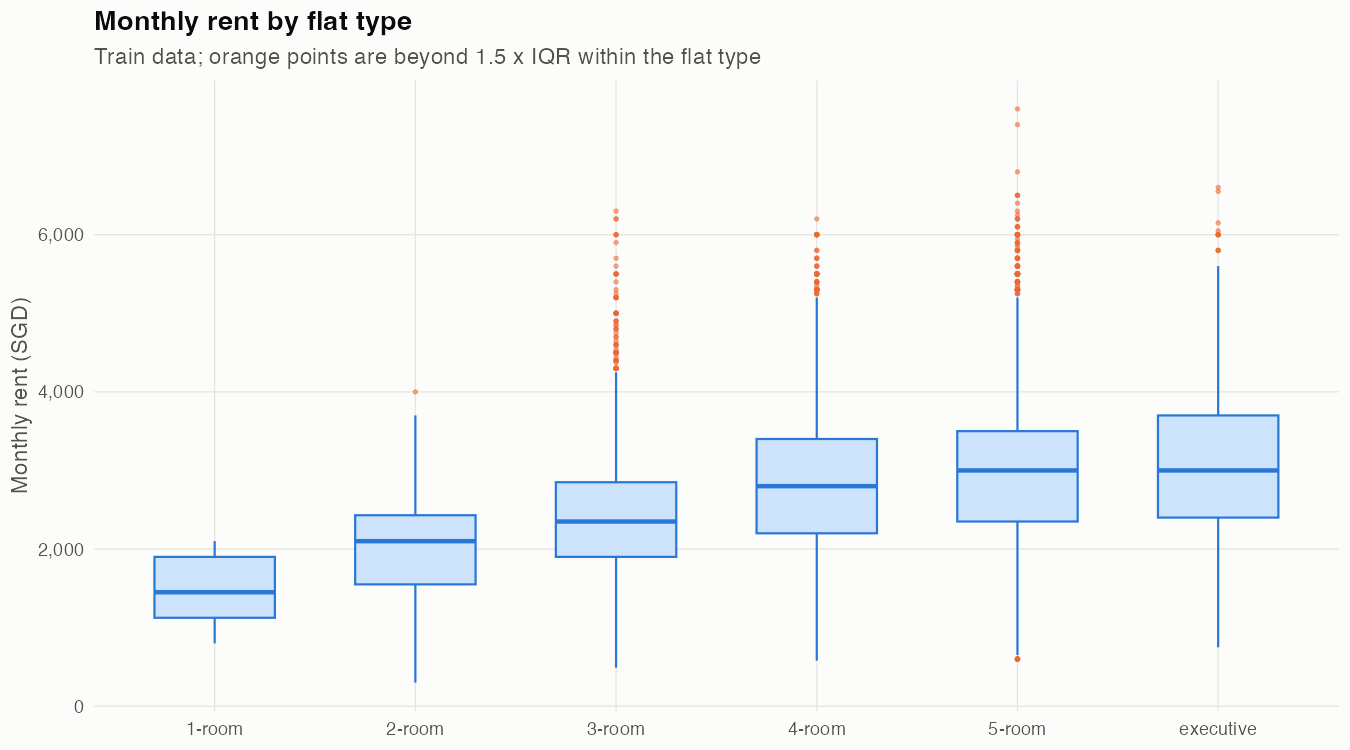
\includegraphics[width=\columnwidth]{../beina/figures/outlier_box_flat_type.png}
\caption{Monthly rent by flat type; points beyond $1.5\times$IQR within the type are shown but kept.\src{Be-out}}\label{fig:box}
\end{figure}

\subsection{Noise floor}
Rows sharing every model input get the same prediction from any deterministic model, so rent spread inside such groups is irreducible. Three groupings give similar estimates: SD 461 for same-unit rentals in one quarter;\src{Be-noise} 464.0 over all labelled months and 454.8 on window P1 for groups sharing all eight inputs;\src{Pu-noise} and 464 for flats in one block, type and month, covering 26.8\% of rows.\src{Aa-noise} Rents are also rounded (87.5\% end in 00), which adds to the noise.\src{Be-round} Our local RMSE of about 450 is of the same order. These estimates cover only rows with a twin and exclude test-period noise.\src{Pu-noise-limit}

\section{Preprocessing and Features}
Table~\ref{tab:eda2prep} traces each exploratory finding to the preprocessing decision it motivated; the pipeline is in Fig.~\ref{fig:flow}.

\begin{table*}[t]
\caption{From exploratory findings to preprocessing decisions.}\label{tab:eda2prep}
\centering\footnotesize
\begin{tabular}{@{}p{5.9cm}p{5.9cm}p{3.6cm}@{}}
\toprule
Finding & Decision & Evidence\\
\midrule
Rent up 53\% then flat; trees cannot extrapolate & Predict the residual over an official median; chronological validation only & Sec.~II-B, Table~\ref{tab:base}\\
COE, stocks and date share only the trend & Drop COE and stocks; never validate on random splits & Sec.~II-C\\
Block-level premiums dominate the residual & Nested shrinkage encodings for block, street and subzone & Table~\ref{tab:imp}\\
Spelling variants (\texttt{STREET} 1,146 to 576 values) & Normalise strings; use native categoricals & Sec.~II-D\\
Sentinel $-1$ values; one bad median entry & Impute from block statistics; remove the entry & Sec.~II-D\\
Outliers are real units and the test set has similar rows & Keep every row; no tail trimming & Sec.~II-D, Table~\ref{tab:matter}\\
Rents rounded; identical flats differ in rent & Treat as a noise floor; do not chase sub-point gains & Sec.~II-E\\
Published medians cover the test quarters & Honest anchor: frozen at 2025-Q1 plus drift & Sec.~III-B, Table~\ref{tab:honest}\\
\bottomrule
\end{tabular}
\end{table*}

\begin{figure*}[t]
\centering
\resizebox{0.98\textwidth}{!}{%
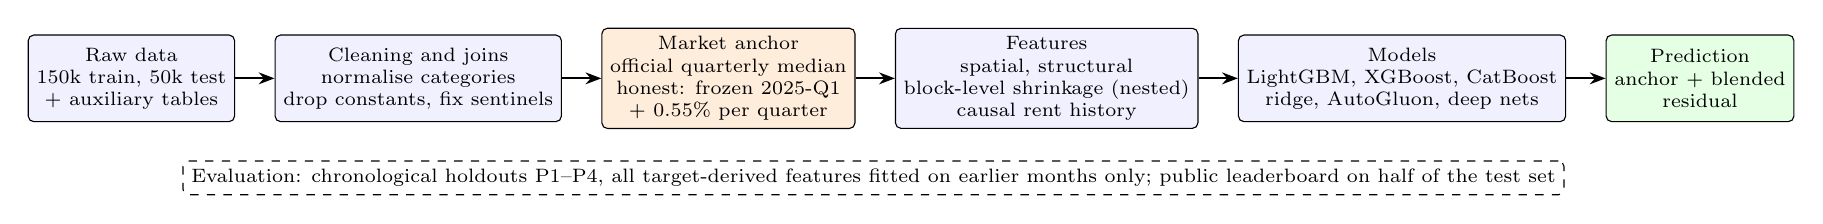
\begin{tikzpicture}[node distance=5mm,
 box/.style={draw,rounded corners=2pt,align=center,minimum height=11mm,font=\scriptsize,fill=blue!6,inner sep=3pt},
 arr/.style={-{Stealth[length=2mm]},thick}]
\node[box] (raw) {Raw data\\150k train, 50k test\\+ auxiliary tables};
\node[box,right=of raw] (clean) {Cleaning and joins\\normalise categories\\drop constants, fix sentinels};
\node[box,right=of clean,fill=orange!14] (anchor) {Market anchor\\official quarterly median\\honest: frozen 2025-Q1\\+ 0.55\% per quarter};
\node[box,right=of anchor] (feat) {Features\\spatial, structural\\block-level shrinkage (nested)\\causal rent history};
\node[box,right=of feat] (model) {Models\\LightGBM, XGBoost, CatBoost\\ridge, AutoGluon, deep nets};
\node[box,right=of model,fill=green!10] (out) {Prediction\\anchor + blended\\residual};
\draw[arr] (raw)--(clean); \draw[arr] (clean)--(anchor); \draw[arr] (anchor)--(feat); \draw[arr] (feat)--(model); \draw[arr] (model)--(out);
\node[draw,dashed,rounded corners=2pt,font=\scriptsize,align=center,below=4mm of feat,xshift=-2.2cm,inner sep=3pt] (ev) {Evaluation: chronological holdouts P1--P4, all target-derived features fitted on earlier months only; public leaderboard on half of the test set};
\end{tikzpicture}}
\caption{Design shared by the four pipelines. The anchor and its honest variant are the central design choice.}\label{fig:flow}
\end{figure*}

\subsection{Cleaning and leakage control}
Rental and block strings are lowercased, trimmed and joined on town, block and street; after normalisation every train and test row matches exactly one block.\src{Be-join} Every target-derived feature for a row in month $t$ uses only labels from months before $t$,\src{Pu-leak} and encoders are fitted inside each training split with inner five-fold out-of-fold values so a row's rent never enters its own feature.\src{Be-te-leak}

\subsection{Market anchor and its honest variant}
The target is rent minus the official median rent for the row's town, flat type and quarter; predictions add it back. Because 51.8\% of the table's values are missing, a fallback chain fills each row: its own cell (96.6\% of train rows), then the national median for the flat type (3.3\%), then adjacent quarters.\src{Be-anchor}

The file runs to 2026-Q2, but a quarter's median aggregates that quarter's rents, so values after the last labelled quarter feed test-period information into the anchor.\src{Be-leak} Our first submission (V2) used them.\src{Aa-v2anchor} The honest variant freezes each cell at 2025-Q1 and multiplies by $\exp(g\,k)$ for $k$ quarters ahead, where $g$ is the mean quarterly log growth of a national index over the last four quarters (+0.55\% at 2025-Q1).\src{Be-drift} Our implementation reproduces the published drift values (+0.78\% at 2024-Q2, +0.55\% at 2025-Q1).\src{Aa-drift}

\subsection{Block-level shrinkage encodings}
High-cardinality keys (14,828 block $\times$ flat-type levels, 576 streets) are encoded by empirical-Bayes shrinkage~\cite{micci}\src{Aa-fp,Me-cat} toward their parent key:
\begin{equation}
\hat\mu_k=\frac{n_k\,\bar r_k+M\,\hat\mu_{\mathrm{parent}(k)}}{n_k+M},\label{eq:te}
\end{equation}
where $\bar r_k$ is the mean residual of key $k$. The hierarchy is town ($M{=}30$), block ($10$), block $\times$ flat type ($5$), street ($15$), subzone ($20$).\src{Aa-M} The R pipeline uses the same constants for the shared levels.\src{Be-te} Hand-set constants proved near-optimal: a random-effects fit recovered 16 for street and 21 for subzone (against 15 and 20) and gave no reliable gain elsewhere.\src{Aa-gpb}

\subsection{Other features}
Structural features (floor area, area per room, maximum floor, year completed, flat age) and distances to the nearest MRT station, mall, school and the CBD with counts within radii\src{Be-spatial} are common to all pipelines. In the V2 pipeline these are computed once per unique block with scikit-learn \texttt{BallTree} indexes under the Haversine metric: nearest distance and counts within 0.5, 1 and 2~km for MRT stations (all, operating, planned, multi-line interchange), malls and primary, secondary and top-tier schools, 20 features in all, including inverse-distance proximity scores.\src{Aa-ball} The R pipeline computes the same kinds of distances independently. The history pipeline adds a 24-month global rent lag and smoothed town $\times$ flat-type and block $\times$ flat-type means with counts; removing the property-level history raises RMSE by 4.388.\src{Pu-hist,Pu-hist-abl} The earlier single-LightGBM root pipeline adds an address-level trailing rent per square metre, which lowers its validation RMSE from 456.70 to 452.56.\src{Aa-addr} The AutoGluon pipeline adds nearest-place names.\src{Me-feat}

\section{Data Mining Methods}
\subsection{Models}
Tabular data with mixed numeric and high-cardinality categorical inputs and 150,000 rows suits boosted trees; trees remain strongest on medium-sized tabular data~\cite{grinsztajn}, and under time-based splits gradient-boosted trees and embedding MLPs rank best~\cite{tabred}. We use LightGBM~\cite{lightgbm}, XGBoost~\cite{xgboost} and CatBoost~\cite{catboost} (ordered target statistics), ridge regression, FT-Transformer~\cite{ftt}, TabTransformer~\cite{tabt}, MLPs, a Temporal Fusion Transformer~\cite{tft} for segment-level forecasts, neural gates and segmented models. The AutoGluon pipeline's AutoGluon-Tabular~\cite{autogluon} setup restricts its base models to LightGBM and CatBoost; AutoGluon's second-level weighted ensemble learns global blend weights, unlike the input-dependent neural gates tested separately, and is extended in later experiments with stacked residual layers. We also reproduced a delayed neural network for Singapore housing prices~\cite{wang2016}.\src{Me-families,Be-paper} Empirical-Bayes target encoding~\cite{micci} and its regularised, cross-fitted forms~\cite{pargent} are standard for high-cardinality keys; random-effects boosting~\cite{gpboost} is the likelihood-based counterpart, which we test in Section~\ref{sec:matter}.

\textbf{Categorical handling.} Categoricals are passed natively to the tree learners; this beat one-hot encoding in six of seven configurations (town, region and block: 481.89 against 482.09),\src{Me-onehot} and replacing every categorical by its target mean was 6.1 to 10.7 RMSE worse.\src{Me-te-all} In the AutoGluon pipeline's selected configuration, automatic text feature generation is disabled with the \texttt{ignore\_text} preset. Thus fields such as street and nearest-MRT name remain categorical, without automatically generated text-special or n-gram columns.\src{Me-text} Encodings of block-like keys are the exception, because they carry information no other feature has (Table~\ref{tab:imp}). Missing numeric block attributes fall back to the town--street median, then the town median, then the global median.\src{Me-fallback}

\subsection{Automated Feature-Selection Experiments}
After establishing a compact manual subset of structurally meaningful property, time, location and accessibility variables, the AutoGluon pipeline evaluated automated selection on a broader 36-variable pool. Two wrapper methods were tested: permutation-importance recursive feature elimination (RFE), which repeatedly refitted the LightGBM--CatBoost ensemble before removing weak variables, and SHAP ranking followed by top-$k$ refits. Chronological rank correlation, mutual information and matched ablations provided supporting diagnostics rather than full-period correlation alone. PCA and truncated SVD were used only as diagnostics because their leading components were not temporally stable. Test labels were never used for selection.\src{Me-fs-manual,Me-fs-auto,Me-dim}

\subsection{Choice of baseline for the residual}
A residual target only helps if the baseline carries the right level. Table~\ref{tab:base} compares baselines across pipelines. A national-level baseline, even an oracle one that knows the actual national average, is worse than the official town $\times$ flat-type median,\src{Be-two-stage} and the history pipeline's residual over a global 24-month lag collapses (CatBoost 662.5 against 464.2 for direct prediction) because the lag lacks town and flat-type detail.\src{Pu-lagres} An explicit trend-plus-residual network is likewise weaker than direct deep prediction (518.6 against 495.9).\src{Me-trendres} Predicting a ratio instead of a difference gave no gain (change $-0.02$).\src{Be-impr}

\begin{table}[t]
\caption{Baselines for the residual target (RMSE).\src{Be-two-stage,Pu-lagres}}\label{tab:base}
\centering\footnotesize
\begin{tabular}{@{}p{4.6cm}p{2.9cm}@{}}
\toprule
Baseline (protocol) & RMSE\\
\midrule
Town $\times$ flat-type official median (P2) & 452.19\\
National level, last 3 months carried forward & 461.99\\
National level, oracle (actual average) & 459.07\\
National level, linear trend & 556.33\\
\midrule
Global 24-month lag, LightGBM / CatBoost (P1): residual & 646.6 / 662.5\\
\hspace{1.2em}same models, direct prediction & 470.8 / 464.2\\
\bottomrule
\end{tabular}
\end{table}

\subsection{Hyperparameters}
The V2 pipeline fixes its settings (LightGBM 1,200 trees, 75 leaves, rate 0.04, early stopping on each fold's validation split).\src{Aa-hp} The R pipeline ran 12, 10 and 6-trial random searches for LightGBM, XGBoost and CatBoost;\src{Be-hp} the history pipeline fixed three LightGBM capacities and three CatBoost seeds and early-stops on the validation window;\src{Pu-hp} the AutoGluon pipeline used 25 trials per model family, supplying the validation period as tuning data.\src{Me-hpo} On the root pipeline a grid, two random searches and a 100-trial Optuna~\cite{optuna} search all fell inside the cross-validation noise: Optuna's best configuration scored 453.71 against 452.56 for the shipped one.\src{Aa-optuna}

\subsection{Blending and final system}
Weights are fitted on out-of-fold or validation predictions: SLSQP in the V2 pipeline (0.545, 0.075, 0.380 for LightGBM, XGBoost, CatBoost),\src{Aa-w} softmax-constrained in the R pipeline,\src{Be-blend} non-negative bounded to $[0,0.85]$ in the history pipeline.\src{Pu-blend}

\textbf{Final models.} We selected two final submissions. The first is five-fold bagged LightGBM, XGBoost and CatBoost on the residual over the \emph{honest} anchor, with the weights above. It scored 433.65480 on the public leaderboard, 0.048 above the version that used published test-quarter medians.\src{Aa-final,Aa-honest-lb} The second is the R pipeline's honest-anchor blend, the version its report adopts; the same setup with COE and stocks scored 433.89670, and the final run without them had not been scored when that report was written.\src{Be-final}

\section{Evaluation and Interpretation}
\subsection{Protocols}
The pipelines used different chronological splits (Table~\ref{tab:proto}); scores compare only within a protocol. Early stopping, candidate selection and blend weights use the validation labels in every pipeline, so local scores are model-selection scores, not untouched estimates; only the leaderboard is independent, and it covers half the test rows.\src{Pu-sel,Me-sel} RMSE is the competition metric; differences are tested with a paired bootstrap that resamples block--month groups (300 draws in the V2 pipeline; 2,000 group resamples in the history pipeline) because rows in one group share unit-level noise.\src{Aa-boot,Pu-noise}

\begin{table}[t]
\caption{Validation protocols.}\label{tab:proto}
\centering\footnotesize
\begin{tabular}{@{}llp{4.6cm}@{}}
\toprule
ID & Pipelines & Fit / validate\\
\midrule
P1 & AutoGluon, history & before 2024-05 (117,988) / 2024-05 to 2025-03 (32,012)\src{Me-split,Pu-W}\\
P2 & V2, R & through 2024-06 (124,016) / 2024-07 to 2025-03 (25,984)\src{Be-split,Aa-e2split}\\
P3 & V2, history (W2) & before 2024-10 (132,802) / 2024-10 to 2025-03 (17,198); the root pipeline drops 641 duplicate rows\src{Pu-W,Aa-dup}\\
P4 & V2 & through 2023-11 / 2023-12 to 2025-03 (16 months)\src{Aa-honest-cost}\\
\bottomrule
\end{tabular}
\end{table}

\subsection{Model comparison}
Table~\ref{tab:results} gives representative results. On P1 the boosted-tree ensemble with causal rent history (463.2) beats AutoGluon without HPO (467.1) by 4 RMSE, and every deep model, gate or router is worse: the best deep expert scores 477.0, TabTransformer 495.9, and segmenting by town or flat type loses 4.6 to 7.6 against the global control.\src{Pu-me,Me-res,Me-seg} On P2 the anchor-and-encoding recipe reaches 450--452 with published medians and 454.9 with the honest anchor, and the R pipeline gives 449.65 and 454.72.\src{Be-res,Aa-honest-cost} On P3, the V2-recipe LightGBM scores 443.64 against 448.688 for the history pipeline's detailed LightGBM, but the first uses published medians and the second none, so the two are not like-for-like.\src{Aa-tab,Pu-w2} A Temporal Fusion Transformer forecasts town $\times$ flat-type monthly means well (RMSE 258.453, $R^2$ 0.8400 on 1,340 segment-months), but adding a listing-level residual model is worse than predicting listings directly (499.791 against 471.209).\src{Me-tft}

\begin{table}[t]
\caption{Representative local RMSE (SGD) by protocol. $^\dagger$published medians; $^\ddagger$honest anchor.\src{Aa-tab,Be-res,Me-res,Pu-me,Pu-w2}}\label{tab:results}
\centering\footnotesize
\begin{tabular}{@{}l@{\hspace{4pt}}l@{\hspace{4pt}}p{3.2cm}r@{}}
\toprule
Prot. & Pipeline & Model & RMSE\\
\midrule
P1 & History & CatBoost, best single seed & 463.549\\
P1 & History & blend v2 / + \sgd/sqm model (v3) & 463.155 / 462.906\\
P1 & AutoGluon & 18 features, no HPO & 467.122\\
P1 & AutoGluon & + one weighted residual layer & 468.057\\
P1 & AutoGluon & deep experts: best / equal blend & 476.979 / 471.168\\
P1 & AutoGluon & TabTransformer & 495.853\\
P2 & R & ridge / LightGBM$^\dagger$ & 451.95 / 452.29\\
P2 & R & XGBoost / CatBoost$^\dagger$ & 450.97 / 450.27\\
P2 & R & blend$^\dagger$ / blend$^\ddagger$ (3 seeds) & 449.65 / 454.72\\
P2 & V2 & CatBoost / LightGBM$^\dagger$ & 450.43 / 452.48\\
P2 & V2 & blend 0.2/0.8$^\dagger$ / blend$^\ddagger$ & 450.30 / 454.85\\
P3 & History & blend v2 / detailed LightGBM & 443.3 / 448.688\\
P3 & V2 & LightGBM$^\dagger$ & 443.64\\
\bottomrule
\end{tabular}
\end{table}

\subsection{Automated Feature-Selection Results}
The controlled manual screen selected a compact 13-variable subset at RMSE 467.230, ahead of the 31-variable full table at 467.507 and the 25-variable candidate expansion at 468.304. The selected production representation subsequently extended the compact set with a prior-only town $\times$ flat-type mean, a global 24-month rent lag and three nearest-place names; its default LightGBM--CatBoost ensemble scored 467.122. Because training budgets and automatic text handling differed between these stages, the latter comparison is a development progression rather than a pure one-variable ablation.\src{Me-fs-manual}

Automated reduction did not establish a stronger independent result. RFE retained all 36 candidates at 468.921; reducing to 10 produced 469.080, while intermediate subsets were less stable. Under the same shortened protocol, the SHAP top-18 subset scored 467.841 against 468.272 for the manual 18-variable set. This 0.431 improvement was selected on the same outer validation period, so it was not treated as an untouched estimate and did not replace the production representation. PCA showed the same temporal-instability warning: the first numeric component's target correlation fell from 0.654 in fitting to 0.306 in validation, and no PCA/SVD replacement-model RMSE was recorded.\src{Me-fs-auto,Me-dim}

\begin{table}[t]
\caption{Automated Feature-selection results on P1.\src{Me-fs-manual,Me-fs-auto}}\label{tab:feature-selection}
\centering\footnotesize
\begin{tabular}{@{}p{2.0cm}p{3.9cm}r@{}}
\toprule
Method & Selected / matched comparator & RMSE\\
\midrule
Manual subsets & Compact 13 / full 31 & 467.230 / 467.507\\
RFE & All 36 / reduced 10 & 468.921 / 469.080\\
SHAP top-$k$ & Top 18 / manual 18 & 467.841 / 468.272\\
\bottomrule
\end{tabular}
\end{table}

\subsection{Alternative Modelling Approaches}
Table~\ref{tab:alternatives} compares the principal alternatives evaluated in the AutoGluon pipeline on the common P1 listing holdout.
Hard segmentation did not help: routing AutoGluon by town and flat type scored 475.846 and 476.068, against global controls of 468.272 and 471.448.
The same pattern held for random forests: the global model scored 484.923, flat-type routing scored 486.073, and chronological tuning improved the global forest to 479.319 but left it well behind boosted trees.
Splitting the data therefore lost more shared signal than it gained from local specialisation.\src{Me-seg,Me-alt}

Deep tabular models learned useful structure but remained weaker than tree ensembles. The best individual deep expert, 
an FT-Transformer, scored 476.979; TabTransformer scored 495.853, while averaging three deep experts improved to 471.168. 
A block-to-town neural gate scored 475.130, so input-dependent routing was again inferior to a fixed blend. The standalone FT-Transformer run scored 497.497, 
and an explicit neural trend-plus-residual decomposition scored 518.590.\src{Me-res,Me-trendres,Me-alt}

Asymmetric and residual-specialist models also showed the value of shrinkage. Quantile LightGBM at $q{=}0.60$ reduced MAE from 356.438 to 343.087 
and shifted predictions toward over-forecasting, but worsened RMSE from 478.370 to 492.281. Weighted flat-type residual experts 
made a small improvement over their matched Layer-1 control (468.272 to 468.068); the significant-residual gate scored 468.360 and the unweighted segmented correction 
deteriorated to 472.509. Thus residual models helped only when their corrections were strongly attenuated.\src{Me-alt}

Time-series experiments used different targets or holdouts and are not included in Table~\ref{tab:alternatives}. A property-group time-series ensemble scored 477.592 
on observed item-months. A town $\times$ flat-type market forecast reached 273.240 at segment level, but its listing hybrid scored 486.052. Likewise, TFT reached 258.453 on segment-month means, 
yet TFT plus a listing residual scored 499.791 against 471.209 for direct listing prediction. Under rolling-origin evaluation, an explicit trend-plus-residual model scored 571.673 against 567.562 for the direct baseline. 
Aggregate temporal patterns were learnable, but their errors compounded when forecasts were translated back to individual listings.\src{Me-tft,Me-alt}

\begin{table}[t]
\caption{Alternative listing-level models evaluated using validation RMSE under the P1 protocol.\src{Me-res,Me-seg,Me-alt}}\label{tab:alternatives}
\centering\scriptsize
\begin{tabular}{@{}p{1.45cm}p{5.05cm}r@{}}
\toprule
Approach & Model description & P1 RMSE\\
\midrule
Reference & AutoGluon LightGBM--CatBoost, default settings & \textbf{467.122}\\
Residual specialists & Weighted flat-type residual experts & 468.068\\
 & Significant-residual gated specialist & 468.360\\
Fixed / learned blends & Equal LightGBM--CatBoost blend & 468.740\\
 & Equal deep-expert blend & 471.168\\
 & Neural LightGBM--CatBoost gate & 472.274\\
 & Block-to-town deep gate & 475.130\\
Hard segmentation & Town-routed AutoGluon & 475.846\\
 & Flat-type-routed AutoGluon & 476.068\\
Random forests & Chronologically tuned random forest & 479.319\\
 & Global random forest & 484.923\\
 & Flat-type-routed random forest & 486.073\\
Asymmetric loss & Quantile LightGBM ($q{=}0.60$) & 492.281\\
Deep tabular & TabTransformer & 495.853\\
 & FT-Transformer & 497.497\\
\bottomrule
\end{tabular}
\end{table}

\subsection{What mattered and what did not}\label{sec:matter}
Table~\ref{tab:matter} separates the changes that moved the score from those that did not. The anchor is decisive over a long horizon: on P4 it cuts RMSE from 600.72 to 492.77, while on a 6-month window the gain is not significant.\src{Aa-anchor} Target encodings, mostly at block level, are the other component that matters: removing all seven costs 8.68 RMSE for the blend and 19.47 for ridge,\src{Be-te-abl} and the step from V1 to V2, which added hierarchical encodings (and interchange-distance features), is the only visible jump on the leaderboard (Fig.~\ref{fig:lb}).\src{Aa-lb} Almost everything else lies within about one RMSE or is worse. Tuning moves results by under 1.2 in the R pipeline's experiments, and recency weighting is reliably worse because it discards block information.\src{Be-impr} Table~\ref{tab:imp} shows where the signal sits: the encodings dominate, the benchmark features come next, and COE and stocks contribute nothing.

\begin{table}[t]
\caption{Permutation importance by feature group: increase in out-of-time RMSE when shuffled (CatBoost, R pipeline).}\label{tab:imp}
\centering\footnotesize
\begin{tabular}{@{}lr@{\hspace{1.4em}}lr@{}}
\toprule
Group & $\Delta$ & Group & $\Delta$\\
\midrule
All 7 encodings & +40.4 & Flat model & +2.1\\
Location encodings & +34.2 & MRT & +1.4\\
Benchmark features & +13.1 & Time & +0.1\\
Flat age, lease year & +6.2 & Stocks & $-0.06$\\
CBD distance & +5.7 & COE & $-0.08$\\
\bottomrule
\end{tabular}\src{Be-imp}
\end{table}

\begin{table*}[t]
\caption{Effect of changes on RMSE (positive = worse). CI = paired-bootstrap 95\% interval; n.s. = not significant.}\label{tab:matter}
\centering\footnotesize
\begin{tabular}{@{}p{5.8cm}p{5.6cm}p{4.0cm}@{}}
\toprule
Change & Effect & Where measured\\
\midrule
Residual over anchor, long horizon & 600.72 $\to$ 492.77\src{Aa-anchor} & P4, root pipeline\\
Residual over anchor, 6-month window & 452.56 $\to$ 451.87 (CI $-1.98$ to $+0.52$, n.s.)\src{Aa-anchor} & P3, root pipeline\\
Target encodings removed (7 keys, mostly block-level) & +8.68 blend, +19.47 ridge\src{Be-te-abl} & P2 (R)\\
Property-level rent history removed & +4.388\src{Pu-hist-abl} & P1 (history)\\
Address-level trailing feature added & $-4.14$ (456.70 $\to$ 452.56)\src{Aa-addr} & P3, root pipeline\\
\midrule
Optuna, 100 trials, vs shipped configuration & +1.15 (453.71 vs 452.56)\src{Aa-optuna} & P3, root pipeline\\
Huber, Fair, L1 losses (Huber $\delta{=}1000$ ties) & +0.7 to +4.9\src{Aa-robust} & P2, P4\\
Trimming 0.5--2.5\% from each tail & +1.7 to +10.6\src{Aa-trim} & P2, P4\\
Random-effects model (GPBoost) replacing encodings & +5.26 and +7.98\src{Aa-gpb} & P2, P4\\
External resale premium by block / neighbour-block priors & $-0.56$, $-0.15$ (n.s.) / $-0.25$ (n.s.), +0.82\src{Aa-resale} & P2, P4\\
Neural gate vs equal blend; town / flat-type routing & +3.5; +7.6 / +4.6\src{Me-res,Me-seg} & P1 (AutoGluon)\\
Prediction-as-feature second layer; AdaBoost residual & +69.9; +29.1\src{Me-stack} & P1 (AutoGluon)\\
Recency weighting (24-month half-life) & +1.14\src{Be-impr} & P2 (R)\\
CatBoost-heavy blend weights & $-0.51$ / $-1.09$ locally, public score +0.023\src{Aa-cbw,Aa-lb} & P2, P4; leaderboard\\
Honest instead of published anchor & +4.55 (P2), public score +0.048\src{Aa-honest-cost,Aa-honest-lb} & P2; leaderboard\\
\bottomrule
\end{tabular}
\end{table*}

\subsection{Local gains against the leaderboard}
Fig.~\ref{fig:lb} shows every submission. The anchor-and-encoding pipelines, the causal-history pipeline and the AutoGluon LightGBM--CatBoost stack fall within 433.4 to 436.3, a plateau only 0.7\% wide. Three local gains of 0.5 to 3 RMSE (deeper trees, premium and bagging, CatBoost-heavy weights) did not appear on the leaderboard (434.05, 434.03, 433.63 against V2's 433.61),\src{Aa-lb,Aa-cbw,Aa-trim} consistent with the public score covering half the test rows and unit-level noise dominating.\src{Pu-lb-limit} Published studies find public leaderboards rank reliably despite adaptive reuse~\cite{roelofs} but that tiny differences carry little information~\cite{ladder}.

\begin{figure}[t]
\centering
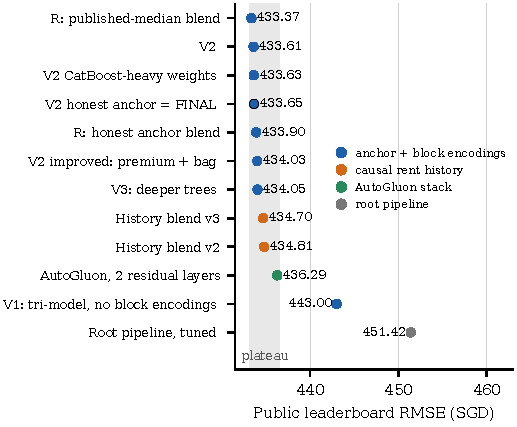
\includegraphics[width=\columnwidth]{figures/fig_leaderboard.pdf}
\caption{Public leaderboard RMSE of every submission by pipeline. The final model is outlined.\src{Aa-lb,Be-lb,Pu-lb,Me-lb}}\label{fig:lb}
\end{figure}

\subsection{Honest anchor}
Table~\ref{tab:honest} quantifies the cost of removing test-period information on the V2 recipe. On P2 it is 4.6 to 6.3 RMSE, matching the R pipeline's measurement of about 5 locally and 0.5 on the leaderboard.\src{Aa-honest-cost,Be-honest-lb} Drift helps when the market is flat (mean error falls from +47.6 to +1.8) but is catastrophic after a surge: at the 2023-Q3 cutoff $g$ was +5.05\% per quarter and extrapolating it over six quarters over-predicted by 885 by 2025-Q1. At the true cutoff $g$ is only +0.55\%, the flat case. The same fragility appears in the history pipeline's backtests, where projected market indices help in one regime and hurt in another.\src{Pu-backtest}

\begin{table}[t]
\caption{Anchor variants, blend 0.2 LightGBM / 0.8 CatBoost (RMSE).\src{Aa-honest-cost}}\label{tab:honest}
\centering\footnotesize
\begin{tabular}{@{}lccc@{}}
\toprule
Holdout & Published & Frozen & Frozen + drift\\
\midrule
P2 ($g{=}{+}0.78\%$) & 450.30 & 456.57 & 454.85\\
P4 ($g{=}{+}5.05\%$) & 482.53 & 487.48 & 764.71\\
\bottomrule
\end{tabular}
\end{table}

\subsection{Data volume and recency}
More real data helps much more than tuning: RMSE falls by roughly 6 to 8 per doubling of training rows (465.77 at 13k rows to 443.64 at 133k) with no sign of saturation, and training that ends 9, 12 or 15 months earlier costs 0.92, 1.84 and 4.17 against a same-size recent sample (Fig.~\ref{fig:learn}).\src{Aa-learn} Block premiums are estimated from few transactions (about 8 rows per block-type level), which is the likely reason for the appetite for data. This also explains why synthetic rows cannot help: the gain comes from real transactions at specific blocks.

\begin{figure}[t]
\centering
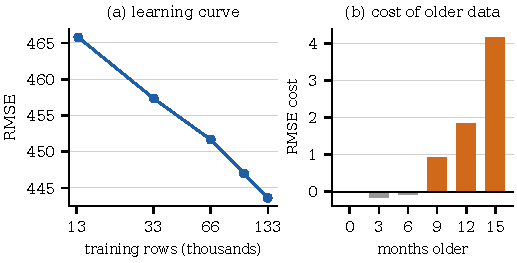
\includegraphics[width=\columnwidth]{figures/fig_learning.pdf}
\caption{(a) RMSE against training rows for V2's recipe on the 2024-10 to 2025-03 window; (b) cost of training data that ends earlier, against a same-size sample.\src{Aa-learn}}\label{fig:learn}
\end{figure}

\subsection{Where the model fails}
Error is concentrated (Fig.~\ref{fig:resid}). On the root pipeline the 6.5\% of validation rows with rent at or below \sgd 2,100 have RMSE 1,090 against 370 for the rest, and so carry 37.5\% of the squared error.\src{Aa-tail} The AutoGluon pipeline's out-of-fold diagnostics show the same pattern by segment: executive flats have RMSE 720, five-room 653 and three-room 542.\src{Me-seg-err} Within a block, flat type and month, rents differ with SD 464, so most of this is not recoverable from the available columns.\src{Aa-noise} The history pipeline finds that on rows with an exact twin, RMSE (452.8) lies inside the interval for the noise estimate (442.2 to 466.8), and that rows without a twin score 14.1 worse, which noise and headroom cannot separate.\src{Pu-twin} Table~\ref{tab:backtest} shows the level error in a rising market. A model that ignores the market also lags: in a rising-market backtest the history pipeline under-predicts by 312 on average, and supplying the true index cuts RMSE from 629.9 to 500.2.\src{Pu-backtest}

\begin{table}[t]
\caption{Moving-market backtests of the history pipeline: 12-month windows after each origin, LightGBM fitted on all earlier rows. Bias is prediction minus actual; the oracle index deflates the target by a market index that includes the validation months.}\label{tab:backtest}
\centering\footnotesize
\begin{tabular}{@{}lccc@{}}
\toprule
Origin & 2022-01 & 2023-01 & 2024-01\\
\midrule
Rent change & +30.0\% & +5.5\% & +2.0\%\\
Control RMSE & 629.9 & 629.1 & 493.9\\
Control bias & $-312.2$ & $-152.0$ & +14.2\\
Oracle RMSE & 500.2 & 604.6 & 490.6\\
Noise SD & 471.3 & 588.5 & 479.3\\
\bottomrule
\end{tabular}\src{Pu-backtest}
\end{table}

\begin{figure}[t]
\centering
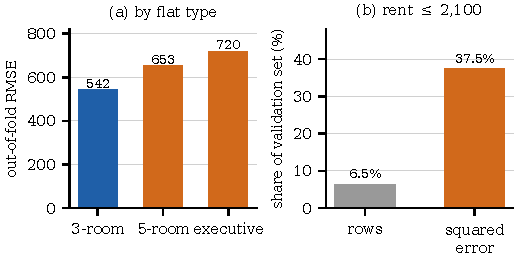
\includegraphics[width=\columnwidth]{figures/fig_errors.pdf}
\caption{Where the error sits: (a) out-of-fold RMSE by flat type (AutoGluon pipeline); (b) the 6.5\% of validation rows with rent at or below \sgd 2,100 carry 37.5\% of the squared error (root pipeline).\src{Me-seg-err,Aa-tail}}\label{fig:resid}
\end{figure}

\textbf{Answers to the research questions.} \textbf{Q1:} the official town $\times$ flat-type median as a residual baseline, with block-level shrinkage encodings, carries the level: public RMSE 443.0 to 433.6 and, over a 16-month holdout, 600.72 to 492.77.\src{Aa-lb,Aa-anchor} \textbf{Q2:} almost nothing else adds more than about one RMSE (Table~\ref{tab:matter}), although more real data does help (Fig.~\ref{fig:learn}). \textbf{Q3:} identical flats differ with SD 455--464 against our local RMSE of about 450, so little headroom remains.\src{Pu-noise,Aa-noise} \textbf{Q4:} local gains of 0.5 to 3 did not reach the leaderboard, and the honest anchor costs 4.6 locally but 0.05 publicly, so local protocols both over- and under-state differences; paired intervals and the leaderboard should be read together.\src{Aa-lb,Aa-honest-cost,Aa-honest-lb}

\section{Limitations and Future Work}
\textbf{Evaluation.} Every local score reuses validation labels for selection;\src{Pu-sel} protocols differ across pipelines; and the test-period market level is unmeasured, since the history pipeline's leaderboard shift probe was never scored.\src{Pu-probe} \textbf{Anchor.} The published medians leak test-period aggregates; our honest variant costs little on the leaderboard but its drift rule is regime-dependent. \textbf{Information.} No dataset we could use legitimately separates units within a block: the official rental registry carries the same fields as ours and the target itself, which is why we did not use it, and block-level data cannot tell two flats in one block apart.\cite{hdbrent} Resale-derived signals and neighbour-block priors gave under one RMSE.\src{Aa-resale} \textbf{Future work:} unit-level data (floor, condition) if the course permits it, regime-aware drift selection, recency-aware encodings, and uncertainty estimates for the heavy low-rent tail.

\textbf{Conclusion.} Carrying the market level through an official median anchor and shrinking block-level premiums toward their parents account for the only large gain we found; everything built on top sits inside a noise floor of about 455--464 SGD that our three groupings measure consistently. The honest forecast-time version of the same model scores 433.65480.

\begin{thebibliography}{99}
\bibitem{hdbrent} Housing and Development Board, ``Renting out of flats,'' data.gov.sg, \url{https://data.gov.sg/dataset/renting-out-of-flats}, accessed Oct. 2026.
\bibitem{grinsztajn} L. Grinsztajn, E. Oyallon and G. Varoquaux, ``Why do tree-based models still outperform deep learning on typical tabular data?'' in \emph{Proc. NeurIPS}, 2022.
\bibitem{tabred} I. Rubachev \emph{et al.}, ``TabReD: Analyzing pitfalls and filling the gaps in tabular deep learning benchmarks,'' in \emph{Proc. ICLR}, 2025.
\bibitem{lightgbm} G. Ke \emph{et al.}, ``LightGBM: A highly efficient gradient boosting decision tree,'' in \emph{Proc. NeurIPS}, 2017.
\bibitem{xgboost} T. Chen and C. Guestrin, ``XGBoost: A scalable tree boosting system,'' in \emph{Proc. KDD}, 2016.
\bibitem{catboost} L. Prokhorenkova \emph{et al.}, ``CatBoost: Unbiased boosting with categorical features,'' in \emph{Proc. NeurIPS}, 2018.
\bibitem{autogluon} N. Erickson \emph{et al.}, ``AutoGluon-Tabular: Robust and accurate AutoML for structured data,'' arXiv:2003.06505, 2020.
\bibitem{ftt} Y. Gorishniy, I. Rubachev, V. Khrulkov and A. Babenko, ``Revisiting deep learning models for tabular data,'' in \emph{Proc. NeurIPS}, 2021.
\bibitem{tabt} X. Huang, A. Khetan, M. Cvitkovic and Z. Karnin, ``TabTransformer: Tabular data modeling using contextual embeddings,'' arXiv:2012.06678, 2020.
\bibitem{tft} B. Lim, S. {\"O}. Ar{\i}k, N. Loeff and T. Pfister, ``Temporal fusion transformers for interpretable multi-horizon time series forecasting,'' \emph{Int. J. Forecasting}, vol. 37, no. 4, pp. 1748--1764, 2021.
\bibitem{wang2016} L. Wang, F. F. Chan, Y. Wang and Q. Chang, ``Predicting public housing prices using delayed neural networks,'' in \emph{Proc. IEEE TENCON}, 2016, pp. 3589--3592.
\bibitem{micci} D. Micci-Barreca, ``A preprocessing scheme for high-cardinality categorical attributes in classification and prediction problems,'' \emph{ACM SIGKDD Explor.}, vol. 3, no. 1, pp. 27--32, 2001.
\bibitem{optuna} T. Akiba, S. Sano, T. Yanase, T. Ohta and M. Koyama, ``Optuna: A next-generation hyperparameter optimization framework,'' in \emph{Proc. KDD}, 2019.
\bibitem{pargent} F. Pargent, F. Pfisterer, J. Thomas and B. Bischl, ``Regularized target encoding outperforms traditional methods in supervised machine learning with high cardinality features,'' \emph{Computational Statistics}, 2022, arXiv:2104.00629.
\bibitem{gpboost} F. Sigrist, ``Gaussian process boosting,'' \emph{J. Mach. Learn. Res.}, vol. 23, no. 232, pp. 1--46, 2022.
\bibitem{roelofs} R. Roelofs \emph{et al.}, ``A meta-analysis of overfitting in machine learning,'' in \emph{Proc. NeurIPS}, 2019.
\bibitem{ladder} A. Blum and M. Hardt, ``The Ladder: A reliable leaderboard for machine learning competitions,'' in \emph{Proc. ICML}, 2015.
\end{thebibliography}

\clearpage
\appendices
\section{Workload}\label{app:work}
\begin{table}[h]
\centering\footnotesize
\begin{tabular}{@{}lp{6.0cm}@{}}
\toprule
Member & Main responsibility\\
\midrule
Aayush & Root pipeline and data-quality audit; median-rent residual anchor and its honest forecast-time variant; V2 recipe (hierarchical shrinkage encodings, BallTree spatial features, three-model blend) and leaderboard series; final submission and the end-to-end reproducible \texttt{main.py}; ablations (tail trimming, robust losses, GPBoost, resale, learning curve)\\
Metul & Shared preprocessing; association, mutual-information and PCA analysis; AutoGluon, deep tabular, gating, segmentation, time-series and residual-stack experiments\\
Punyaa & Leakage-safe causal rent-history features; LightGBM/CatBoost ensemble and 76 unit tests; extrapolation, noise-floor and moving-market backtests\\
Beina & R cleaning and EDA; in-fold hierarchical encodings; honest-anchor drift; ablations and feature importance; the second selected final submission (\texttt{predict\_test.R})\\
\bottomrule
\end{tabular}
\end{table}
\emph{This table summarises the content of each member's folder under \texttt{report/}; each member should confirm it.}\src{Wk-P,Wk-M,Wk-B}

\section{Hyperparameters and reproduction}
V2: LightGBM 1,200 trees, 75 leaves, learning rate 0.04, subsample 0.8, column sample 0.75; XGBoost depth 7; CatBoost 1,200 iterations, depth 7, learning rate 0.05; early stopping 40 rounds; five folds, seed 42.\src{Aa-v2hp} The final model is reproduced end to end, from the raw files to \url{submission.csv}, by \url{main.py} with the code in \url{modules/}.\src{Aa-main} Experiment scripts: \url{expt-2/src/models_v2.py} (V2), \url{expt-5/src/honest_v2_submission.py} (honest anchor), \url{expt-5/src/exp6_honest_anchor_validation.py} (Table~\ref{tab:honest}). History pipeline: \url{python3 -m punyaa.train}; R pipeline: \url{model_training.R}, \url{predict_test.R}; AutoGluon pipeline: notebooks under \url{exploration/metul}.\src{Pu-repro,Be-scripts,Me-trace}

\end{document}
"  to show them, plain  pdflatex main  hides them ----
\newif\ifshowsrc
\ifdefined\SHOWSRC\showsrctrue\else\showsrcfalse\fi
\newcommand{\src}[1]{\ifshowsrc\textsuperscript{\tiny\color{gray}[#1]}\fi}

\newcommand{\sgd}{S\$}
\def\BibTeX{{\rm B\kern-.05em{\sc i\kern-.025em b}\kern-.08em T\kern-.1667em\lower.7ex\hbox{E}\kern-.125emX}}

\begin{document}
\pagestyle{plain}
\pagenumbering{arabic}

\title{Forecasting HDB Rents Sixteen Months Ahead:\\Market Anchors, Block-Level Shrinkage and the Noise Floor\\[2pt]\large Team 2 --- [TEAM NAME]}

\author{\IEEEauthorblockN{Aayush Majumdar}
\IEEEauthorblockA{\textit{Student ID A0352046L}\\
\textit{National University of Singapore}}
\and
\IEEEauthorblockN{Metul Prabhu}
\IEEEauthorblockA{\textit{Student ID A0352394Y}\\
\textit{National University of Singapore}}
\and
\IEEEauthorblockN{Punyaa [Surname]}
\IEEEauthorblockA{\textit{Student ID [ID]}\\
\textit{National University of Singapore}}
\and
\IEEEauthorblockN{Beina [Surname]}
\IEEEauthorblockA{\textit{Student ID [ID]}\\
\textit{National University of Singapore}}}

\maketitle
\thispagestyle{plain}

\begin{abstract}
We forecast the monthly rent of 50,000 Singapore HDB flat rentals approved up to sixteen months after our 150,000 labelled examples (2021--2025). We built four pipelines on the same data: gradient-boosted trees on the residual over an official median rent with block-level shrinkage encodings, causal rent-history features, AutoGluon LightGBM--CatBoost stacks plus deep tabular models, and an R pipeline with the first design. Three findings emerge. First, predicting the residual over the official median rent, with block-level encodings, is the only change that moved the public leaderboard materially (443.0 to 433.6 RMSE). Second, deep models, gating, segmentation, hyperparameter search, robust losses, tail trimming and external resale data each moved RMSE by about one point or made it worse. Third, identical flats rent with a standard deviation of about 455--464 SGD, the same order as our error. The released median-rent file covers the test quarters and so leaks future aggregates; an honest forecast-time anchor costs about 5 RMSE locally but 0.05 on the leaderboard. Our final model scores 433.65480.\src{Aa-lb,Aa-honest-lb,Aa-honest-cost,Be-noise,Pu-noise,Aa-noise,Me-families}
\end{abstract}

\section{Introduction}
Rents of public housing are a visible measure of living costs, and the Housing and Development Board (HDB) publishes every approved flat rental as open data~\cite{hdbrent}. A model that predicts a flat's rent helps tenants and owners judge asking rents and helps analysts follow the market. We predict the monthly rent of 50,000 rental approvals dated March 2025 to July 2026 from 150,000 labelled approvals dated January 2021 to March 2025, plus auxiliary tables on blocks, MRT stations, malls, schools, COE premiums, stock prices and official median rents.\src{Pu-task,Be-inputs}

Three properties make the task hard. (i) The test months lie up to sixteen months after the last label,\src{Pu-future} while rents rose 53\% over the labelled period and then flattened.\src{Be-trend} (ii) Location carries most of the signal at a finer grain than any single numeric feature.\src{Be-weakcorr} (iii) Flats that look identical in the data rent for different amounts.\src{Pu-noise}

We ask four questions. \textbf{Q1:} what information lets a model carry the market level to unseen months? \textbf{Q2:} how much can better models add on top? \textbf{Q3:} how much of the error is irreducible? \textbf{Q4:} how far can local validation be trusted against an external leaderboard? We call the four pipelines V2 (boosted trees on the residual over the official median), R (the same design in R), history (causal rent-history features) and AutoGluon (stacks and deep tabular models).

\section{Data and Exploratory Analysis}
\subsection{Data}
Table~\ref{tab:data} lists the inputs. Only eight raw columns vary (approval month, town, block, street, flat type, flat model, floor area, lease start); \texttt{FURNISHED} and \texttt{FEE} are constant and are dropped.\src{Pu-task}

\begin{table}[t]
\caption{Data used.}\label{tab:data}
\centering\footnotesize
\begin{tabular}{@{}p{2.3cm}p{5.2cm}@{}}
\toprule
File & Content\\
\midrule
train / test & 150,000 rentals (2021-01 to 2025-03) / 50,000 (2025-03 to 2026-07)\src{Be-inputs}\\
HDB blocks & 9,464 blocks: coordinates, maximum floor, year completed, subzone\src{Be-inputs}\\
MRT, malls, schools & 243 stations, 113 malls, 337 schools\src{Be-inputs}\\
COE, stocks & monthly premiums, daily prices (tested, not retained)\\
Median rent & 13,305 quarterly values by town and flat type, 51.8\% missing\src{Be-anchor}\\
\bottomrule
\end{tabular}
\end{table}

\subsection{Market drift}
Mean rent rose 53\%, from \sgd 2,055 (first three months) to \sgd 3,142 (last three), nearly all of it between mid-2021 and mid-2023; it has been almost flat since.\src{Be-trend} The official town $\times$ flat-type median follows the level closely (Fig.~\ref{fig:trend}). Trees cannot extrapolate a trend,\src{Pu-trees} so every strong model here predicts the residual over this benchmark instead of rent itself.

\begin{figure}[t]
\centering
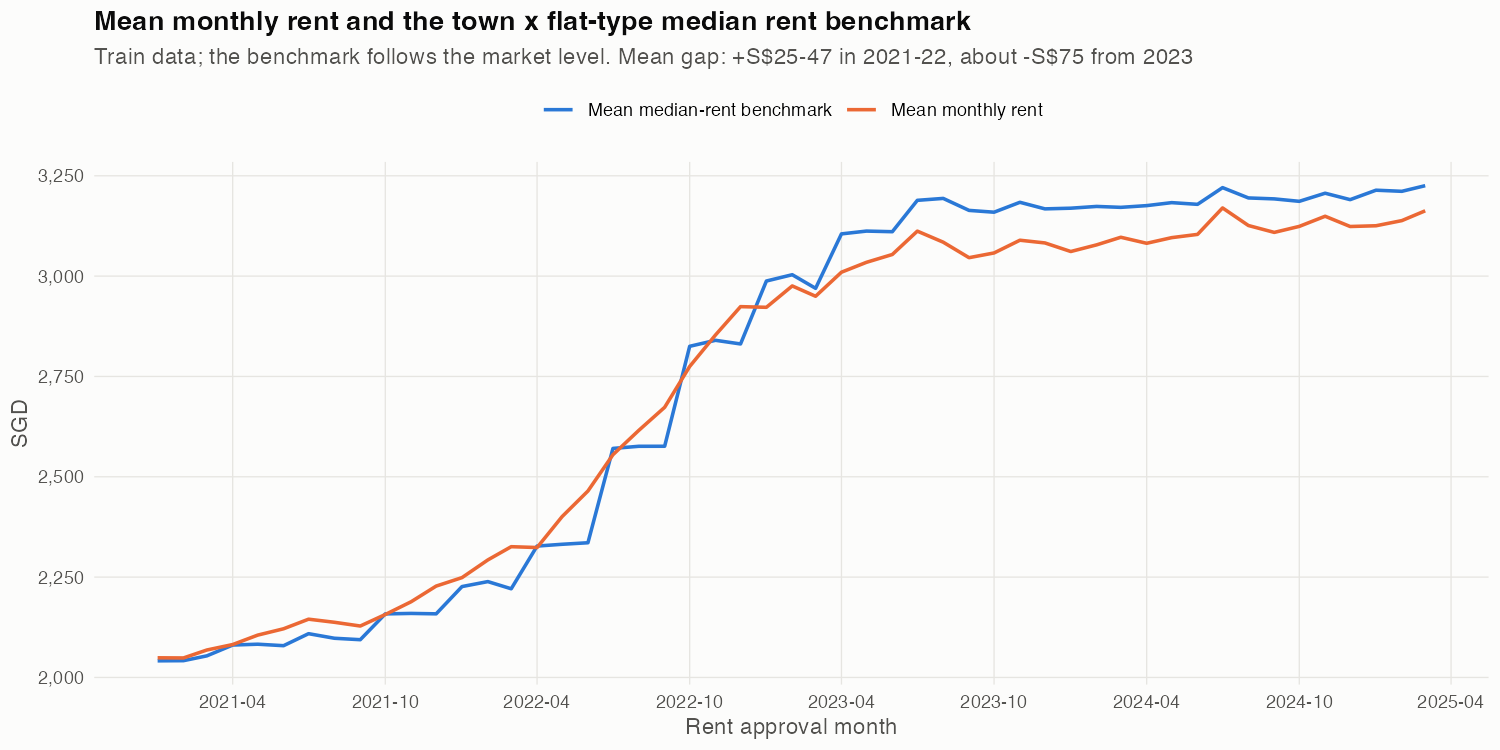
\includegraphics[width=\columnwidth]{../beina/figures/trend_rent_vs_benchmark.png}
\caption{Mean monthly rent and the mean town $\times$ flat-type median benchmark (train months).\src{Be-trend}}\label{fig:trend}
\end{figure}

\subsection{Calendar and macro proxies}
Approval date, COE premium and stock prices correlate strongly with rent over the whole period only because they share the trend. COE correlates 0.898 with monthly mean rent in levels but 0.015 in month-on-month changes.\src{Be-coe} Inside the validation period their rank correlation with rent collapses (COE 0.528 to 0.006, approval date 0.562 to 0.018), whereas the town $\times$ flat-type historical mean keeps 0.664 to 0.668 (Fig.~\ref{fig:assoc}).\src{Me-assoc} Mutual information with rent likewise ranks that historical mean first (0.361), ahead of approval date (0.229) and COE premium (0.218).\src{Me-mi} COE and stocks have negative permutation importance ($-0.08$, $-0.06$) and are dropped.\src{Be-imp} A random split would hide this failure, so all validation is chronological.

\begin{figure}[t]
\centering
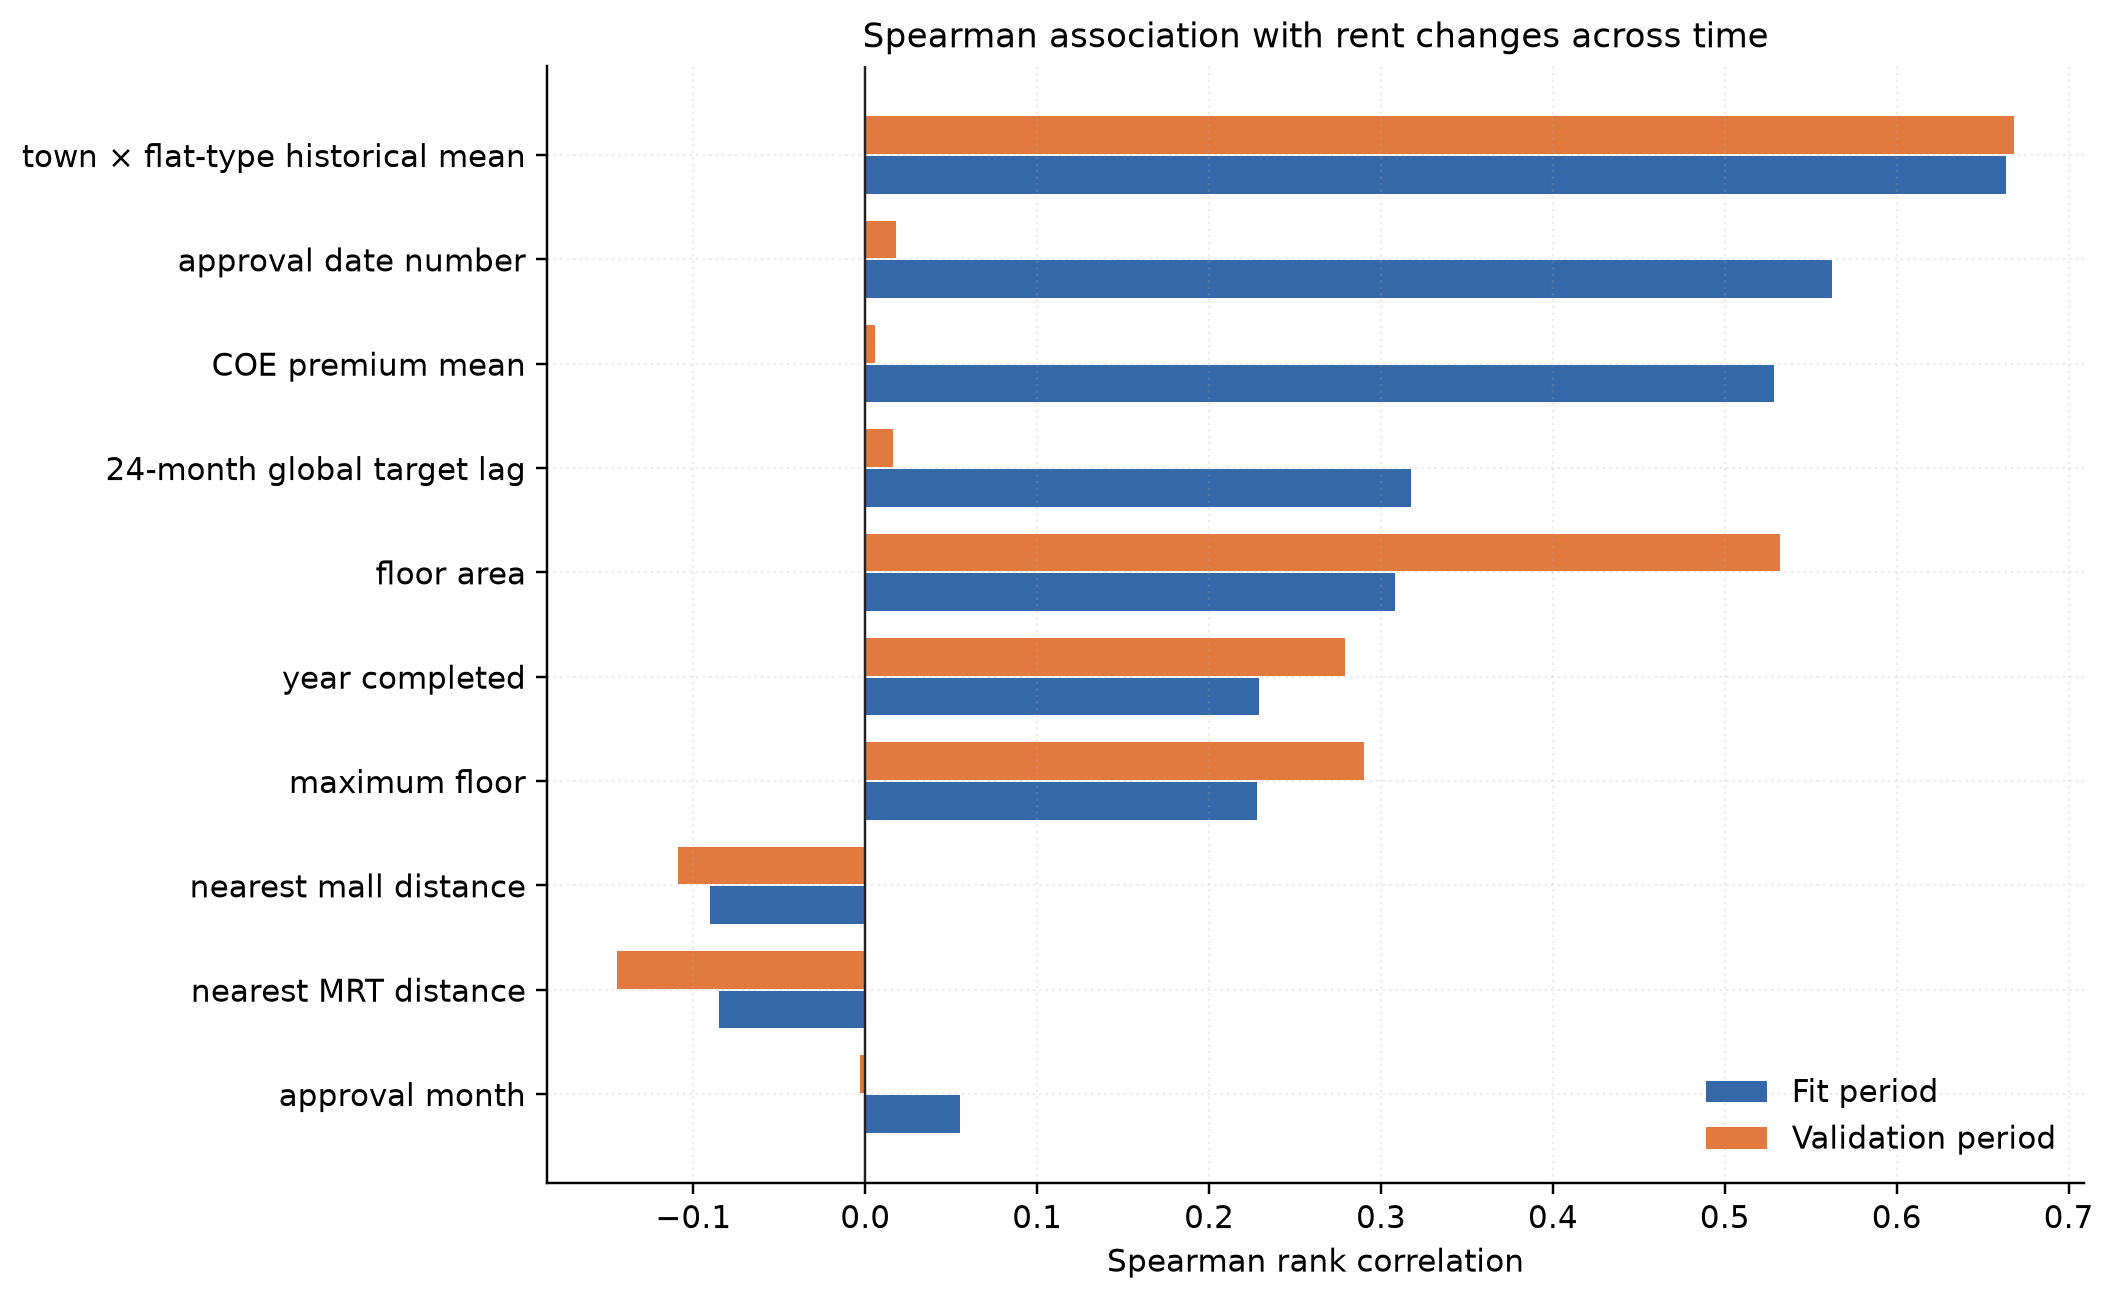
\includegraphics[width=\columnwidth]{../metul/figures/association_stability.png}
\caption{Spearman correlation with rent in the fitting and chronological validation periods (P1 protocol).\src{Me-assoc}}\label{fig:assoc}
\end{figure}

\subsection{Location, categories and outliers}
Once the benchmark is removed the numeric features correlate weakly with the residual ($|r|\le 0.12$), so the remainder is mostly block-level.\src{Be-weakcorr} Shuffling the seven target encodings (mostly block-level) raises out-of-time RMSE by 40.4, the largest effect of any feature group; the four location encodings alone account for 34.2.\src{Be-imp}

Lowercasing and normalising separators cuts \texttt{STREET} from 1,146 to 576 values and \texttt{FLAT\_TYPE} from 11 to 6.\src{Me-cat} Every test town, street, flat type and model occurs in training; 11 unseen block labels affect 36 of 50,000 test rows (0.072\%).\src{Me-cov} Without normalising address casing, 30,781 train rows (20.5\%) fail to join to the block table.\src{Be-join} Eleven blocks store $-1$ for maximum floor and year completed (159 train rows) and are imputed; one median entry (300 against about 3,000 elsewhere) is removed.\src{Be-sent,Be-bad}

We keep every row. The IQR rule flags 130 floor areas and 752 rents,\src{Me-out} but only 0.11\% of rows are extreme relative to their benchmark. The highest rents are real adjoined flats and premium maisonettes, the lowest (\sgd 300--450) are 2-room flats that are probably subsidised or room rentals.\src{Be-out} Removing training tails also hurt RMSE at every level we tried (Section~\ref{sec:matter}).

\begin{figure}[t]
\centering
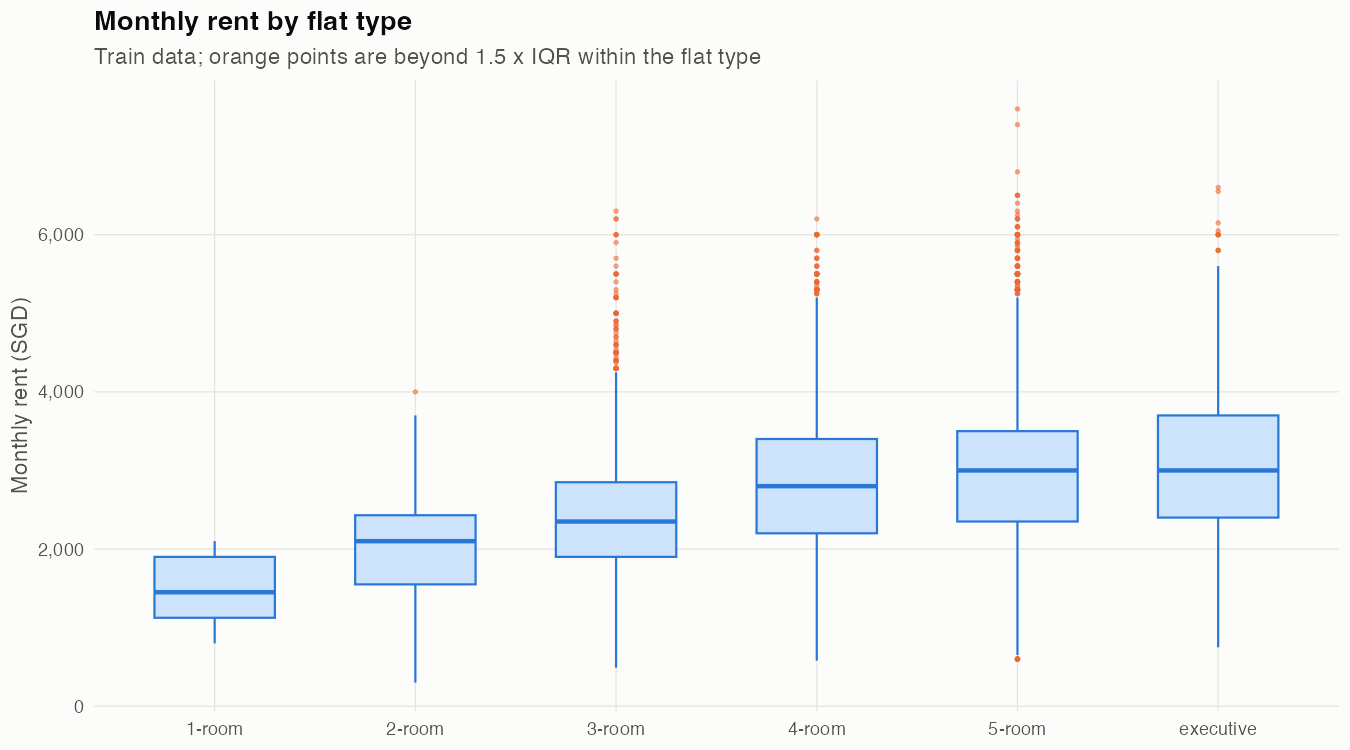
\includegraphics[width=\columnwidth]{../beina/figures/outlier_box_flat_type.png}
\caption{Monthly rent by flat type; points beyond $1.5\times$IQR within the type are shown but kept.\src{Be-out}}\label{fig:box}
\end{figure}

\subsection{Noise floor}
Rows sharing every model input get the same prediction from any deterministic model, so rent spread inside such groups is irreducible. Three groupings give similar estimates: SD 461 for same-unit rentals in one quarter;\src{Be-noise} 464.0 over all labelled months and 454.8 on window P1 for groups sharing all eight inputs;\src{Pu-noise} and 464 for flats in one block, type and month, covering 26.8\% of rows.\src{Aa-noise} Rents are also rounded (87.5\% end in 00), which adds to the noise.\src{Be-round} Our local RMSE of about 450 is of the same order. These estimates cover only rows with a twin and exclude test-period noise.\src{Pu-noise-limit}

\section{Preprocessing and Features}
Table~\ref{tab:eda2prep} traces each exploratory finding to the preprocessing decision it motivated; the pipeline is in Fig.~\ref{fig:flow}.

\begin{table*}[t]
\caption{From exploratory findings to preprocessing decisions.}\label{tab:eda2prep}
\centering\footnotesize
\begin{tabular}{@{}p{5.9cm}p{5.9cm}p{3.6cm}@{}}
\toprule
Finding & Decision & Evidence\\
\midrule
Rent up 53\% then flat; trees cannot extrapolate & Predict the residual over an official median; chronological validation only & Sec.~II-B, Table~\ref{tab:base}\\
COE, stocks and date share only the trend & Drop COE and stocks; never validate on random splits & Sec.~II-C\\
Block-level premiums dominate the residual & Nested shrinkage encodings for block, street and subzone & Table~\ref{tab:imp}\\
Spelling variants (\texttt{STREET} 1,146 to 576 values) & Normalise strings; use native categoricals & Sec.~II-D\\
Sentinel $-1$ values; one bad median entry & Impute from block statistics; remove the entry & Sec.~II-D\\
Outliers are real units and the test set has similar rows & Keep every row; no tail trimming & Sec.~II-D, Table~\ref{tab:matter}\\
Rents rounded; identical flats differ in rent & Treat as a noise floor; do not chase sub-point gains & Sec.~II-E\\
Published medians cover the test quarters & Honest anchor: frozen at 2025-Q1 plus drift & Sec.~III-B, Table~\ref{tab:honest}\\
\bottomrule
\end{tabular}
\end{table*}

\begin{figure*}[t]
\centering
\resizebox{0.98\textwidth}{!}{%
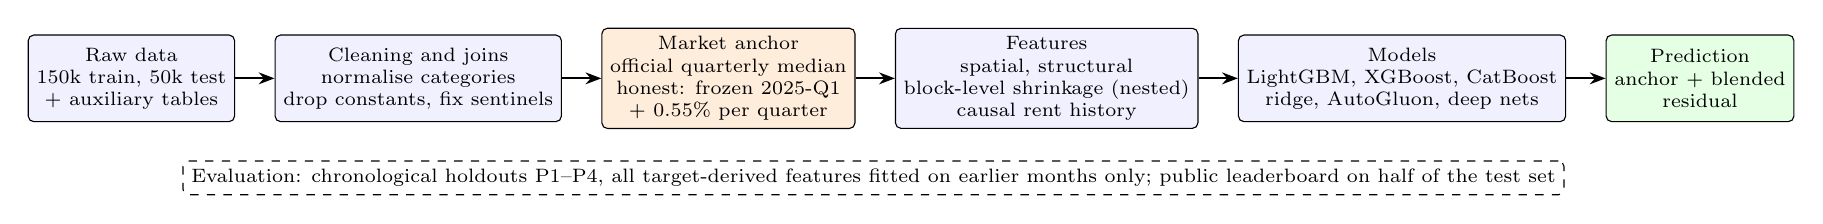
\begin{tikzpicture}[node distance=5mm,
 box/.style={draw,rounded corners=2pt,align=center,minimum height=11mm,font=\scriptsize,fill=blue!6,inner sep=3pt},
 arr/.style={-{Stealth[length=2mm]},thick}]
\node[box] (raw) {Raw data\\150k train, 50k test\\+ auxiliary tables};
\node[box,right=of raw] (clean) {Cleaning and joins\\normalise categories\\drop constants, fix sentinels};
\node[box,right=of clean,fill=orange!14] (anchor) {Market anchor\\official quarterly median\\honest: frozen 2025-Q1\\+ 0.55\% per quarter};
\node[box,right=of anchor] (feat) {Features\\spatial, structural\\block-level shrinkage (nested)\\causal rent history};
\node[box,right=of feat] (model) {Models\\LightGBM, XGBoost, CatBoost\\ridge, AutoGluon, deep nets};
\node[box,right=of model,fill=green!10] (out) {Prediction\\anchor + blended\\residual};
\draw[arr] (raw)--(clean); \draw[arr] (clean)--(anchor); \draw[arr] (anchor)--(feat); \draw[arr] (feat)--(model); \draw[arr] (model)--(out);
\node[draw,dashed,rounded corners=2pt,font=\scriptsize,align=center,below=4mm of feat,xshift=-2.2cm,inner sep=3pt] (ev) {Evaluation: chronological holdouts P1--P4, all target-derived features fitted on earlier months only; public leaderboard on half of the test set};
\end{tikzpicture}}
\caption{Design shared by the four pipelines. The anchor and its honest variant are the central design choice.}\label{fig:flow}
\end{figure*}

\subsection{Cleaning and leakage control}
Rental and block strings are lowercased, trimmed and joined on town, block and street; after normalisation every train and test row matches exactly one block.\src{Be-join} Every target-derived feature for a row in month $t$ uses only labels from months before $t$,\src{Pu-leak} and encoders are fitted inside each training split with inner five-fold out-of-fold values so a row's rent never enters its own feature.\src{Be-te-leak}

\subsection{Market anchor and its honest variant}
The target is rent minus the official median rent for the row's town, flat type and quarter; predictions add it back. Because 51.8\% of the table's values are missing, a fallback chain fills each row: its own cell (96.6\% of train rows), then the national median for the flat type (3.3\%), then adjacent quarters.\src{Be-anchor}

The file runs to 2026-Q2, but a quarter's median aggregates that quarter's rents, so values after the last labelled quarter feed test-period information into the anchor.\src{Be-leak} Our first submission (V2) used them.\src{Aa-v2anchor} The honest variant freezes each cell at 2025-Q1 and multiplies by $\exp(g\,k)$ for $k$ quarters ahead, where $g$ is the mean quarterly log growth of a national index over the last four quarters (+0.55\% at 2025-Q1).\src{Be-drift} Our implementation reproduces the published drift values (+0.78\% at 2024-Q2, +0.55\% at 2025-Q1).\src{Aa-drift}

\subsection{Block-level shrinkage encodings}
High-cardinality keys (14,828 block $\times$ flat-type levels, 576 streets) are encoded by empirical-Bayes shrinkage~\cite{micci}\src{Aa-fp,Me-cat} toward their parent key:
\begin{equation}
\hat\mu_k=\frac{n_k\,\bar r_k+M\,\hat\mu_{\mathrm{parent}(k)}}{n_k+M},\label{eq:te}
\end{equation}
where $\bar r_k$ is the mean residual of key $k$. The hierarchy is town ($M{=}30$), block ($10$), block $\times$ flat type ($5$), street ($15$), subzone ($20$).\src{Aa-M} The R pipeline uses the same constants for the shared levels.\src{Be-te} Hand-set constants proved near-optimal: a random-effects fit recovered 16 for street and 21 for subzone (against 15 and 20) and gave no reliable gain elsewhere.\src{Aa-gpb}

\subsection{Other features}
Structural features (floor area, area per room, maximum floor, year completed, flat age) and distances to the nearest MRT station, mall, school and the CBD with counts within radii\src{Be-spatial} are common to all pipelines. In the V2 pipeline these are computed once per unique block with scikit-learn \texttt{BallTree} indexes under the Haversine metric: nearest distance and counts within 0.5, 1 and 2~km for MRT stations (all, operating, planned, multi-line interchange), malls and primary, secondary and top-tier schools, 20 features in all, including inverse-distance proximity scores.\src{Aa-ball} The R pipeline computes the same kinds of distances independently. The history pipeline adds a 24-month global rent lag and smoothed town $\times$ flat-type and block $\times$ flat-type means with counts; removing the property-level history raises RMSE by 4.388.\src{Pu-hist,Pu-hist-abl} The earlier single-LightGBM root pipeline adds an address-level trailing rent per square metre, which lowers its validation RMSE from 456.70 to 452.56.\src{Aa-addr} The AutoGluon pipeline adds nearest-place names.\src{Me-feat}

\section{Data Mining Methods}
\subsection{Models}
Tabular data with mixed numeric and high-cardinality categorical inputs and 150,000 rows suits boosted trees; trees remain strongest on medium-sized tabular data~\cite{grinsztajn}, and under time-based splits gradient-boosted trees and embedding MLPs rank best~\cite{tabred}. We use LightGBM~\cite{lightgbm}, XGBoost~\cite{xgboost} and CatBoost~\cite{catboost} (ordered target statistics), ridge regression, FT-Transformer~\cite{ftt}, TabTransformer~\cite{tabt}, MLPs, a Temporal Fusion Transformer~\cite{tft} for segment-level forecasts, neural gates and segmented models. The AutoGluon pipeline's AutoGluon-Tabular~\cite{autogluon} setup restricts its base models to LightGBM and CatBoost; AutoGluon's second-level weighted ensemble learns global blend weights, unlike the input-dependent neural gates tested separately, and is extended in later experiments with stacked residual layers. We also reproduced a delayed neural network for Singapore housing prices~\cite{wang2016}.\src{Me-families,Be-paper} Empirical-Bayes target encoding~\cite{micci} and its regularised, cross-fitted forms~\cite{pargent} are standard for high-cardinality keys; random-effects boosting~\cite{gpboost} is the likelihood-based counterpart, which we test in Section~\ref{sec:matter}.

\textbf{Categorical handling.} Categoricals are passed natively to the tree learners; this beat one-hot encoding in six of seven configurations (town, region and block: 481.89 against 482.09),\src{Me-onehot} and replacing every categorical by its target mean was 6.1 to 10.7 RMSE worse.\src{Me-te-all} In the AutoGluon pipeline's selected configuration, automatic text feature generation is disabled with the \texttt{ignore\_text} preset. Thus fields such as street and nearest-MRT name remain categorical, without automatically generated text-special or n-gram columns.\src{Me-text} Encodings of block-like keys are the exception, because they carry information no other feature has (Table~\ref{tab:imp}). Missing numeric block attributes fall back to the town--street median, then the town median, then the global median.\src{Me-fallback}

\subsection{Automated Feature-Selection Experiments}
After establishing a compact manual subset of structurally meaningful property, time, location and accessibility variables, the AutoGluon pipeline evaluated automated selection on a broader 36-variable pool. Two wrapper methods were tested: permutation-importance recursive feature elimination (RFE), which repeatedly refitted the LightGBM--CatBoost ensemble before removing weak variables, and SHAP ranking followed by top-$k$ refits. Chronological rank correlation, mutual information and matched ablations provided supporting diagnostics rather than full-period correlation alone. PCA and truncated SVD were used only as diagnostics because their leading components were not temporally stable. Test labels were never used for selection.\src{Me-fs-manual,Me-fs-auto,Me-dim}

\subsection{Choice of baseline for the residual}
A residual target only helps if the baseline carries the right level. Table~\ref{tab:base} compares baselines across pipelines. A national-level baseline, even an oracle one that knows the actual national average, is worse than the official town $\times$ flat-type median,\src{Be-two-stage} and the history pipeline's residual over a global 24-month lag collapses (CatBoost 662.5 against 464.2 for direct prediction) because the lag lacks town and flat-type detail.\src{Pu-lagres} An explicit trend-plus-residual network is likewise weaker than direct deep prediction (518.6 against 495.9).\src{Me-trendres} Predicting a ratio instead of a difference gave no gain (change $-0.02$).\src{Be-impr}

\begin{table}[t]
\caption{Baselines for the residual target (RMSE).\src{Be-two-stage,Pu-lagres}}\label{tab:base}
\centering\footnotesize
\begin{tabular}{@{}p{4.6cm}p{2.9cm}@{}}
\toprule
Baseline (protocol) & RMSE\\
\midrule
Town $\times$ flat-type official median (P2) & 452.19\\
National level, last 3 months carried forward & 461.99\\
National level, oracle (actual average) & 459.07\\
National level, linear trend & 556.33\\
\midrule
Global 24-month lag, LightGBM / CatBoost (P1): residual & 646.6 / 662.5\\
\hspace{1.2em}same models, direct prediction & 470.8 / 464.2\\
\bottomrule
\end{tabular}
\end{table}

\subsection{Hyperparameters}
The V2 pipeline fixes its settings (LightGBM 1,200 trees, 75 leaves, rate 0.04, early stopping on each fold's validation split).\src{Aa-hp} The R pipeline ran 12, 10 and 6-trial random searches for LightGBM, XGBoost and CatBoost;\src{Be-hp} the history pipeline fixed three LightGBM capacities and three CatBoost seeds and early-stops on the validation window;\src{Pu-hp} the AutoGluon pipeline used 25 trials per model family, supplying the validation period as tuning data.\src{Me-hpo} On the root pipeline a grid, two random searches and a 100-trial Optuna~\cite{optuna} search all fell inside the cross-validation noise: Optuna's best configuration scored 453.71 against 452.56 for the shipped one.\src{Aa-optuna}

\subsection{Blending and final system}
Weights are fitted on out-of-fold or validation predictions: SLSQP in the V2 pipeline (0.545, 0.075, 0.380 for LightGBM, XGBoost, CatBoost),\src{Aa-w} softmax-constrained in the R pipeline,\src{Be-blend} non-negative bounded to $[0,0.85]$ in the history pipeline.\src{Pu-blend}

\textbf{Final models.} We selected two final submissions. The first is five-fold bagged LightGBM, XGBoost and CatBoost on the residual over the \emph{honest} anchor, with the weights above. It scored 433.65480 on the public leaderboard, 0.048 above the version that used published test-quarter medians.\src{Aa-final,Aa-honest-lb} The second is the R pipeline's honest-anchor blend, the version its report adopts; the same setup with COE and stocks scored 433.89670, and the final run without them had not been scored when that report was written.\src{Be-final}

\section{Evaluation and Interpretation}
\subsection{Protocols}
The pipelines used different chronological splits (Table~\ref{tab:proto}); scores compare only within a protocol. Early stopping, candidate selection and blend weights use the validation labels in every pipeline, so local scores are model-selection scores, not untouched estimates; only the leaderboard is independent, and it covers half the test rows.\src{Pu-sel,Me-sel} RMSE is the competition metric; differences are tested with a paired bootstrap that resamples block--month groups (300 draws in the V2 pipeline; 2,000 group resamples in the history pipeline) because rows in one group share unit-level noise.\src{Aa-boot,Pu-noise}

\begin{table}[t]
\caption{Validation protocols.}\label{tab:proto}
\centering\footnotesize
\begin{tabular}{@{}llp{4.6cm}@{}}
\toprule
ID & Pipelines & Fit / validate\\
\midrule
P1 & AutoGluon, history & before 2024-05 (117,988) / 2024-05 to 2025-03 (32,012)\src{Me-split,Pu-W}\\
P2 & V2, R & through 2024-06 (124,016) / 2024-07 to 2025-03 (25,984)\src{Be-split,Aa-e2split}\\
P3 & V2, history (W2) & before 2024-10 (132,802) / 2024-10 to 2025-03 (17,198); the root pipeline drops 641 duplicate rows\src{Pu-W,Aa-dup}\\
P4 & V2 & through 2023-11 / 2023-12 to 2025-03 (16 months)\src{Aa-honest-cost}\\
\bottomrule
\end{tabular}
\end{table}

\subsection{Model comparison}
Table~\ref{tab:results} gives representative results. On P1 the boosted-tree ensemble with causal rent history (463.2) beats AutoGluon without HPO (467.1) by 4 RMSE, and every deep model, gate or router is worse: the best deep expert scores 477.0, TabTransformer 495.9, and segmenting by town or flat type loses 4.6 to 7.6 against the global control.\src{Pu-me,Me-res,Me-seg} On P2 the anchor-and-encoding recipe reaches 450--452 with published medians and 454.9 with the honest anchor, and the R pipeline gives 449.65 and 454.72.\src{Be-res,Aa-honest-cost} On P3, the V2-recipe LightGBM scores 443.64 against 448.688 for the history pipeline's detailed LightGBM, but the first uses published medians and the second none, so the two are not like-for-like.\src{Aa-tab,Pu-w2} A Temporal Fusion Transformer forecasts town $\times$ flat-type monthly means well (RMSE 258.453, $R^2$ 0.8400 on 1,340 segment-months), but adding a listing-level residual model is worse than predicting listings directly (499.791 against 471.209).\src{Me-tft}

\begin{table}[t]
\caption{Representative local RMSE (SGD) by protocol. $^\dagger$published medians; $^\ddagger$honest anchor.\src{Aa-tab,Be-res,Me-res,Pu-me,Pu-w2}}\label{tab:results}
\centering\footnotesize
\begin{tabular}{@{}l@{\hspace{4pt}}l@{\hspace{4pt}}p{3.2cm}r@{}}
\toprule
Prot. & Pipeline & Model & RMSE\\
\midrule
P1 & History & CatBoost, best single seed & 463.549\\
P1 & History & blend v2 / + \sgd/sqm model (v3) & 463.155 / 462.906\\
P1 & AutoGluon & 18 features, no HPO & 467.122\\
P1 & AutoGluon & + one weighted residual layer & 468.057\\
P1 & AutoGluon & deep experts: best / equal blend & 476.979 / 471.168\\
P1 & AutoGluon & TabTransformer & 495.853\\
P2 & R & ridge / LightGBM$^\dagger$ & 451.95 / 452.29\\
P2 & R & XGBoost / CatBoost$^\dagger$ & 450.97 / 450.27\\
P2 & R & blend$^\dagger$ / blend$^\ddagger$ (3 seeds) & 449.65 / 454.72\\
P2 & V2 & CatBoost / LightGBM$^\dagger$ & 450.43 / 452.48\\
P2 & V2 & blend 0.2/0.8$^\dagger$ / blend$^\ddagger$ & 450.30 / 454.85\\
P3 & History & blend v2 / detailed LightGBM & 443.3 / 448.688\\
P3 & V2 & LightGBM$^\dagger$ & 443.64\\
\bottomrule
\end{tabular}
\end{table}

\subsection{Automated Feature-Selection Results}
The controlled manual screen selected a compact 13-variable subset at RMSE 467.230, ahead of the 31-variable full table at 467.507 and the 25-variable candidate expansion at 468.304. The selected production representation subsequently extended the compact set with a prior-only town $\times$ flat-type mean, a global 24-month rent lag and three nearest-place names; its default LightGBM--CatBoost ensemble scored 467.122. Because training budgets and automatic text handling differed between these stages, the latter comparison is a development progression rather than a pure one-variable ablation.\src{Me-fs-manual}

Automated reduction did not establish a stronger independent result. RFE retained all 36 candidates at 468.921; reducing to 10 produced 469.080, while intermediate subsets were less stable. Under the same shortened protocol, the SHAP top-18 subset scored 467.841 against 468.272 for the manual 18-variable set. This 0.431 improvement was selected on the same outer validation period, so it was not treated as an untouched estimate and did not replace the production representation. PCA showed the same temporal-instability warning: the first numeric component's target correlation fell from 0.654 in fitting to 0.306 in validation, and no PCA/SVD replacement-model RMSE was recorded.\src{Me-fs-auto,Me-dim}

\begin{table}[t]
\caption{Automated Feature-selection results on P1.\src{Me-fs-manual,Me-fs-auto}}\label{tab:feature-selection}
\centering\footnotesize
\begin{tabular}{@{}p{2.0cm}p{3.9cm}r@{}}
\toprule
Method & Selected / matched comparator & RMSE\\
\midrule
Manual subsets & Compact 13 / full 31 & 467.230 / 467.507\\
RFE & All 36 / reduced 10 & 468.921 / 469.080\\
SHAP top-$k$ & Top 18 / manual 18 & 467.841 / 468.272\\
\bottomrule
\end{tabular}
\end{table}

\subsection{Alternative Modelling Approaches}
Table~\ref{tab:alternatives} compares the principal alternatives evaluated in the AutoGluon pipeline on the common P1 listing holdout.
Hard segmentation did not help: routing AutoGluon by town and flat type scored 475.846 and 476.068, against global controls of 468.272 and 471.448.
The same pattern held for random forests: the global model scored 484.923, flat-type routing scored 486.073, and chronological tuning improved the global forest to 479.319 but left it well behind boosted trees.
Splitting the data therefore lost more shared signal than it gained from local specialisation.\src{Me-seg,Me-alt}

Deep tabular models learned useful structure but remained weaker than tree ensembles. The best individual deep expert, 
an FT-Transformer, scored 476.979; TabTransformer scored 495.853, while averaging three deep experts improved to 471.168. 
A block-to-town neural gate scored 475.130, so input-dependent routing was again inferior to a fixed blend. The standalone FT-Transformer run scored 497.497, 
and an explicit neural trend-plus-residual decomposition scored 518.590.\src{Me-res,Me-trendres,Me-alt}

Asymmetric and residual-specialist models also showed the value of shrinkage. Quantile LightGBM at $q{=}0.60$ reduced MAE from 356.438 to 343.087 
and shifted predictions toward over-forecasting, but worsened RMSE from 478.370 to 492.281. Weighted flat-type residual experts 
made a small improvement over their matched Layer-1 control (468.272 to 468.068); the significant-residual gate scored 468.360 and the unweighted segmented correction 
deteriorated to 472.509. Thus residual models helped only when their corrections were strongly attenuated.\src{Me-alt}

Time-series experiments used different targets or holdouts and are not included in Table~\ref{tab:alternatives}. A property-group time-series ensemble scored 477.592 
on observed item-months. A town $\times$ flat-type market forecast reached 273.240 at segment level, but its listing hybrid scored 486.052. Likewise, TFT reached 258.453 on segment-month means, 
yet TFT plus a listing residual scored 499.791 against 471.209 for direct listing prediction. Under rolling-origin evaluation, an explicit trend-plus-residual model scored 571.673 against 567.562 for the direct baseline. 
Aggregate temporal patterns were learnable, but their errors compounded when forecasts were translated back to individual listings.\src{Me-tft,Me-alt}

\begin{table}[t]
\caption{Alternative listing-level models evaluated using validation RMSE under the P1 protocol.\src{Me-res,Me-seg,Me-alt}}\label{tab:alternatives}
\centering\scriptsize
\begin{tabular}{@{}p{1.45cm}p{5.05cm}r@{}}
\toprule
Approach & Model description & P1 RMSE\\
\midrule
Reference & AutoGluon LightGBM--CatBoost, default settings & \textbf{467.122}\\
Residual specialists & Weighted flat-type residual experts & 468.068\\
 & Significant-residual gated specialist & 468.360\\
Fixed / learned blends & Equal LightGBM--CatBoost blend & 468.740\\
 & Equal deep-expert blend & 471.168\\
 & Neural LightGBM--CatBoost gate & 472.274\\
 & Block-to-town deep gate & 475.130\\
Hard segmentation & Town-routed AutoGluon & 475.846\\
 & Flat-type-routed AutoGluon & 476.068\\
Random forests & Chronologically tuned random forest & 479.319\\
 & Global random forest & 484.923\\
 & Flat-type-routed random forest & 486.073\\
Asymmetric loss & Quantile LightGBM ($q{=}0.60$) & 492.281\\
Deep tabular & TabTransformer & 495.853\\
 & FT-Transformer & 497.497\\
\bottomrule
\end{tabular}
\end{table}

\subsection{What mattered and what did not}\label{sec:matter}
Table~\ref{tab:matter} separates the changes that moved the score from those that did not. The anchor is decisive over a long horizon: on P4 it cuts RMSE from 600.72 to 492.77, while on a 6-month window the gain is not significant.\src{Aa-anchor} Target encodings, mostly at block level, are the other component that matters: removing all seven costs 8.68 RMSE for the blend and 19.47 for ridge,\src{Be-te-abl} and the step from V1 to V2, which added hierarchical encodings (and interchange-distance features), is the only visible jump on the leaderboard (Fig.~\ref{fig:lb}).\src{Aa-lb} Almost everything else lies within about one RMSE or is worse. Tuning moves results by under 1.2 in the R pipeline's experiments, and recency weighting is reliably worse because it discards block information.\src{Be-impr} Table~\ref{tab:imp} shows where the signal sits: the encodings dominate, the benchmark features come next, and COE and stocks contribute nothing.

\begin{table}[t]
\caption{Permutation importance by feature group: increase in out-of-time RMSE when shuffled (CatBoost, R pipeline).}\label{tab:imp}
\centering\footnotesize
\begin{tabular}{@{}lr@{\hspace{1.4em}}lr@{}}
\toprule
Group & $\Delta$ & Group & $\Delta$\\
\midrule
All 7 encodings & +40.4 & Flat model & +2.1\\
Location encodings & +34.2 & MRT & +1.4\\
Benchmark features & +13.1 & Time & +0.1\\
Flat age, lease year & +6.2 & Stocks & $-0.06$\\
CBD distance & +5.7 & COE & $-0.08$\\
\bottomrule
\end{tabular}\src{Be-imp}
\end{table}

\begin{table*}[t]
\caption{Effect of changes on RMSE (positive = worse). CI = paired-bootstrap 95\% interval; n.s. = not significant.}\label{tab:matter}
\centering\footnotesize
\begin{tabular}{@{}p{5.8cm}p{5.6cm}p{4.0cm}@{}}
\toprule
Change & Effect & Where measured\\
\midrule
Residual over anchor, long horizon & 600.72 $\to$ 492.77\src{Aa-anchor} & P4, root pipeline\\
Residual over anchor, 6-month window & 452.56 $\to$ 451.87 (CI $-1.98$ to $+0.52$, n.s.)\src{Aa-anchor} & P3, root pipeline\\
Target encodings removed (7 keys, mostly block-level) & +8.68 blend, +19.47 ridge\src{Be-te-abl} & P2 (R)\\
Property-level rent history removed & +4.388\src{Pu-hist-abl} & P1 (history)\\
Address-level trailing feature added & $-4.14$ (456.70 $\to$ 452.56)\src{Aa-addr} & P3, root pipeline\\
\midrule
Optuna, 100 trials, vs shipped configuration & +1.15 (453.71 vs 452.56)\src{Aa-optuna} & P3, root pipeline\\
Huber, Fair, L1 losses (Huber $\delta{=}1000$ ties) & +0.7 to +4.9\src{Aa-robust} & P2, P4\\
Trimming 0.5--2.5\% from each tail & +1.7 to +10.6\src{Aa-trim} & P2, P4\\
Random-effects model (GPBoost) replacing encodings & +5.26 and +7.98\src{Aa-gpb} & P2, P4\\
External resale premium by block / neighbour-block priors & $-0.56$, $-0.15$ (n.s.) / $-0.25$ (n.s.), +0.82\src{Aa-resale} & P2, P4\\
Neural gate vs equal blend; town / flat-type routing & +3.5; +7.6 / +4.6\src{Me-res,Me-seg} & P1 (AutoGluon)\\
Prediction-as-feature second layer; AdaBoost residual & +69.9; +29.1\src{Me-stack} & P1 (AutoGluon)\\
Recency weighting (24-month half-life) & +1.14\src{Be-impr} & P2 (R)\\
CatBoost-heavy blend weights & $-0.51$ / $-1.09$ locally, public score +0.023\src{Aa-cbw,Aa-lb} & P2, P4; leaderboard\\
Honest instead of published anchor & +4.55 (P2), public score +0.048\src{Aa-honest-cost,Aa-honest-lb} & P2; leaderboard\\
\bottomrule
\end{tabular}
\end{table*}

\subsection{Local gains against the leaderboard}
Fig.~\ref{fig:lb} shows every submission. The anchor-and-encoding pipelines, the causal-history pipeline and the AutoGluon LightGBM--CatBoost stack fall within 433.4 to 436.3, a plateau only 0.7\% wide. Three local gains of 0.5 to 3 RMSE (deeper trees, premium and bagging, CatBoost-heavy weights) did not appear on the leaderboard (434.05, 434.03, 433.63 against V2's 433.61),\src{Aa-lb,Aa-cbw,Aa-trim} consistent with the public score covering half the test rows and unit-level noise dominating.\src{Pu-lb-limit} Published studies find public leaderboards rank reliably despite adaptive reuse~\cite{roelofs} but that tiny differences carry little information~\cite{ladder}.

\begin{figure}[t]
\centering
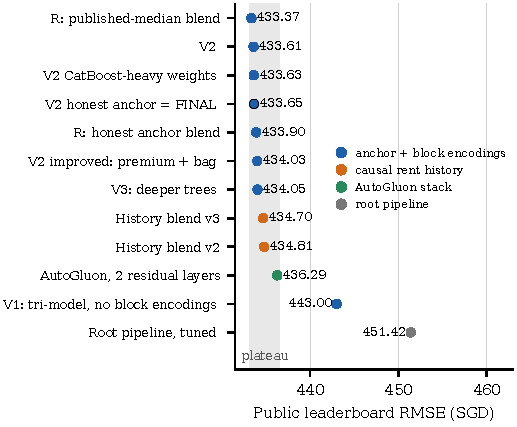
\includegraphics[width=\columnwidth]{figures/fig_leaderboard.pdf}
\caption{Public leaderboard RMSE of every submission by pipeline. The final model is outlined.\src{Aa-lb,Be-lb,Pu-lb,Me-lb}}\label{fig:lb}
\end{figure}

\subsection{Honest anchor}
Table~\ref{tab:honest} quantifies the cost of removing test-period information on the V2 recipe. On P2 it is 4.6 to 6.3 RMSE, matching the R pipeline's measurement of about 5 locally and 0.5 on the leaderboard.\src{Aa-honest-cost,Be-honest-lb} Drift helps when the market is flat (mean error falls from +47.6 to +1.8) but is catastrophic after a surge: at the 2023-Q3 cutoff $g$ was +5.05\% per quarter and extrapolating it over six quarters over-predicted by 885 by 2025-Q1. At the true cutoff $g$ is only +0.55\%, the flat case. The same fragility appears in the history pipeline's backtests, where projected market indices help in one regime and hurt in another.\src{Pu-backtest}

\begin{table}[t]
\caption{Anchor variants, blend 0.2 LightGBM / 0.8 CatBoost (RMSE).\src{Aa-honest-cost}}\label{tab:honest}
\centering\footnotesize
\begin{tabular}{@{}lccc@{}}
\toprule
Holdout & Published & Frozen & Frozen + drift\\
\midrule
P2 ($g{=}{+}0.78\%$) & 450.30 & 456.57 & 454.85\\
P4 ($g{=}{+}5.05\%$) & 482.53 & 487.48 & 764.71\\
\bottomrule
\end{tabular}
\end{table}

\subsection{Data volume and recency}
More real data helps much more than tuning: RMSE falls by roughly 6 to 8 per doubling of training rows (465.77 at 13k rows to 443.64 at 133k) with no sign of saturation, and training that ends 9, 12 or 15 months earlier costs 0.92, 1.84 and 4.17 against a same-size recent sample (Fig.~\ref{fig:learn}).\src{Aa-learn} Block premiums are estimated from few transactions (about 8 rows per block-type level), which is the likely reason for the appetite for data. This also explains why synthetic rows cannot help: the gain comes from real transactions at specific blocks.

\begin{figure}[t]
\centering
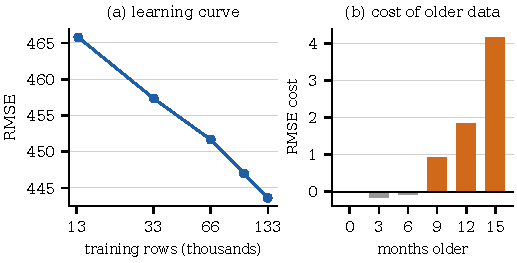
\includegraphics[width=\columnwidth]{figures/fig_learning.pdf}
\caption{(a) RMSE against training rows for V2's recipe on the 2024-10 to 2025-03 window; (b) cost of training data that ends earlier, against a same-size sample.\src{Aa-learn}}\label{fig:learn}
\end{figure}

\subsection{Where the model fails}
Error is concentrated (Fig.~\ref{fig:resid}). On the root pipeline the 6.5\% of validation rows with rent at or below \sgd 2,100 have RMSE 1,090 against 370 for the rest, and so carry 37.5\% of the squared error.\src{Aa-tail} The AutoGluon pipeline's out-of-fold diagnostics show the same pattern by segment: executive flats have RMSE 720, five-room 653 and three-room 542.\src{Me-seg-err} Within a block, flat type and month, rents differ with SD 464, so most of this is not recoverable from the available columns.\src{Aa-noise} The history pipeline finds that on rows with an exact twin, RMSE (452.8) lies inside the interval for the noise estimate (442.2 to 466.8), and that rows without a twin score 14.1 worse, which noise and headroom cannot separate.\src{Pu-twin} Table~\ref{tab:backtest} shows the level error in a rising market. A model that ignores the market also lags: in a rising-market backtest the history pipeline under-predicts by 312 on average, and supplying the true index cuts RMSE from 629.9 to 500.2.\src{Pu-backtest}

\begin{table}[t]
\caption{Moving-market backtests of the history pipeline: 12-month windows after each origin, LightGBM fitted on all earlier rows. Bias is prediction minus actual; the oracle index deflates the target by a market index that includes the validation months.}\label{tab:backtest}
\centering\footnotesize
\begin{tabular}{@{}lccc@{}}
\toprule
Origin & 2022-01 & 2023-01 & 2024-01\\
\midrule
Rent change & +30.0\% & +5.5\% & +2.0\%\\
Control RMSE & 629.9 & 629.1 & 493.9\\
Control bias & $-312.2$ & $-152.0$ & +14.2\\
Oracle RMSE & 500.2 & 604.6 & 490.6\\
Noise SD & 471.3 & 588.5 & 479.3\\
\bottomrule
\end{tabular}\src{Pu-backtest}
\end{table}

\begin{figure}[t]
\centering
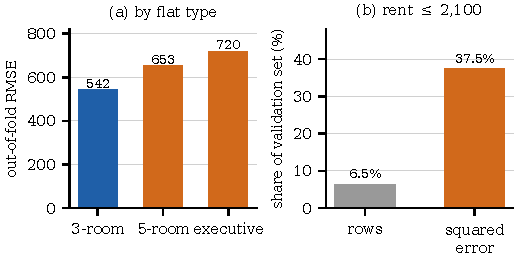
\includegraphics[width=\columnwidth]{figures/fig_errors.pdf}
\caption{Where the error sits: (a) out-of-fold RMSE by flat type (AutoGluon pipeline); (b) the 6.5\% of validation rows with rent at or below \sgd 2,100 carry 37.5\% of the squared error (root pipeline).\src{Me-seg-err,Aa-tail}}\label{fig:resid}
\end{figure}

\textbf{Answers to the research questions.} \textbf{Q1:} the official town $\times$ flat-type median as a residual baseline, with block-level shrinkage encodings, carries the level: public RMSE 443.0 to 433.6 and, over a 16-month holdout, 600.72 to 492.77.\src{Aa-lb,Aa-anchor} \textbf{Q2:} almost nothing else adds more than about one RMSE (Table~\ref{tab:matter}), although more real data does help (Fig.~\ref{fig:learn}). \textbf{Q3:} identical flats differ with SD 455--464 against our local RMSE of about 450, so little headroom remains.\src{Pu-noise,Aa-noise} \textbf{Q4:} local gains of 0.5 to 3 did not reach the leaderboard, and the honest anchor costs 4.6 locally but 0.05 publicly, so local protocols both over- and under-state differences; paired intervals and the leaderboard should be read together.\src{Aa-lb,Aa-honest-cost,Aa-honest-lb}

\section{Limitations and Future Work}
\textbf{Evaluation.} Every local score reuses validation labels for selection;\src{Pu-sel} protocols differ across pipelines; and the test-period market level is unmeasured, since the history pipeline's leaderboard shift probe was never scored.\src{Pu-probe} \textbf{Anchor.} The published medians leak test-period aggregates; our honest variant costs little on the leaderboard but its drift rule is regime-dependent. \textbf{Information.} No dataset we could use legitimately separates units within a block: the official rental registry carries the same fields as ours and the target itself, which is why we did not use it, and block-level data cannot tell two flats in one block apart.\cite{hdbrent} Resale-derived signals and neighbour-block priors gave under one RMSE.\src{Aa-resale} \textbf{Future work:} unit-level data (floor, condition) if the course permits it, regime-aware drift selection, recency-aware encodings, and uncertainty estimates for the heavy low-rent tail.

\textbf{Conclusion.} Carrying the market level through an official median anchor and shrinking block-level premiums toward their parents account for the only large gain we found; everything built on top sits inside a noise floor of about 455--464 SGD that our three groupings measure consistently. The honest forecast-time version of the same model scores 433.65480.

\begin{thebibliography}{99}
\bibitem{hdbrent} Housing and Development Board, ``Renting out of flats,'' data.gov.sg, \url{https://data.gov.sg/dataset/renting-out-of-flats}, accessed Oct. 2026.
\bibitem{grinsztajn} L. Grinsztajn, E. Oyallon and G. Varoquaux, ``Why do tree-based models still outperform deep learning on typical tabular data?'' in \emph{Proc. NeurIPS}, 2022.
\bibitem{tabred} I. Rubachev \emph{et al.}, ``TabReD: Analyzing pitfalls and filling the gaps in tabular deep learning benchmarks,'' in \emph{Proc. ICLR}, 2025.
\bibitem{lightgbm} G. Ke \emph{et al.}, ``LightGBM: A highly efficient gradient boosting decision tree,'' in \emph{Proc. NeurIPS}, 2017.
\bibitem{xgboost} T. Chen and C. Guestrin, ``XGBoost: A scalable tree boosting system,'' in \emph{Proc. KDD}, 2016.
\bibitem{catboost} L. Prokhorenkova \emph{et al.}, ``CatBoost: Unbiased boosting with categorical features,'' in \emph{Proc. NeurIPS}, 2018.
\bibitem{autogluon} N. Erickson \emph{et al.}, ``AutoGluon-Tabular: Robust and accurate AutoML for structured data,'' arXiv:2003.06505, 2020.
\bibitem{ftt} Y. Gorishniy, I. Rubachev, V. Khrulkov and A. Babenko, ``Revisiting deep learning models for tabular data,'' in \emph{Proc. NeurIPS}, 2021.
\bibitem{tabt} X. Huang, A. Khetan, M. Cvitkovic and Z. Karnin, ``TabTransformer: Tabular data modeling using contextual embeddings,'' arXiv:2012.06678, 2020.
\bibitem{tft} B. Lim, S. {\"O}. Ar{\i}k, N. Loeff and T. Pfister, ``Temporal fusion transformers for interpretable multi-horizon time series forecasting,'' \emph{Int. J. Forecasting}, vol. 37, no. 4, pp. 1748--1764, 2021.
\bibitem{wang2016} L. Wang, F. F. Chan, Y. Wang and Q. Chang, ``Predicting public housing prices using delayed neural networks,'' in \emph{Proc. IEEE TENCON}, 2016, pp. 3589--3592.
\bibitem{micci} D. Micci-Barreca, ``A preprocessing scheme for high-cardinality categorical attributes in classification and prediction problems,'' \emph{ACM SIGKDD Explor.}, vol. 3, no. 1, pp. 27--32, 2001.
\bibitem{optuna} T. Akiba, S. Sano, T. Yanase, T. Ohta and M. Koyama, ``Optuna: A next-generation hyperparameter optimization framework,'' in \emph{Proc. KDD}, 2019.
\bibitem{pargent} F. Pargent, F. Pfisterer, J. Thomas and B. Bischl, ``Regularized target encoding outperforms traditional methods in supervised machine learning with high cardinality features,'' \emph{Computational Statistics}, 2022, arXiv:2104.00629.
\bibitem{gpboost} F. Sigrist, ``Gaussian process boosting,'' \emph{J. Mach. Learn. Res.}, vol. 23, no. 232, pp. 1--46, 2022.
\bibitem{roelofs} R. Roelofs \emph{et al.}, ``A meta-analysis of overfitting in machine learning,'' in \emph{Proc. NeurIPS}, 2019.
\bibitem{ladder} A. Blum and M. Hardt, ``The Ladder: A reliable leaderboard for machine learning competitions,'' in \emph{Proc. ICML}, 2015.
\end{thebibliography}

\clearpage
\appendices
\section{Workload}\label{app:work}
\begin{table}[h]
\centering\footnotesize
\begin{tabular}{@{}lp{6.0cm}@{}}
\toprule
Member & Main responsibility\\
\midrule
Aayush & Root pipeline and data-quality audit; median-rent residual anchor and its honest forecast-time variant; V2 recipe (hierarchical shrinkage encodings, BallTree spatial features, three-model blend) and leaderboard series; final submission and the end-to-end reproducible \texttt{main.py}; ablations (tail trimming, robust losses, GPBoost, resale, learning curve)\\
Metul & Shared preprocessing; association, mutual-information and PCA analysis; AutoGluon, deep tabular, gating, segmentation, time-series and residual-stack experiments\\
Punyaa & Leakage-safe causal rent-history features; LightGBM/CatBoost ensemble and 76 unit tests; extrapolation, noise-floor and moving-market backtests\\
Beina & R cleaning and EDA; in-fold hierarchical encodings; honest-anchor drift; ablations and feature importance; the second selected final submission (\texttt{predict\_test.R})\\
\bottomrule
\end{tabular}
\end{table}
\emph{This table summarises the content of each member's folder under \texttt{report/}; each member should confirm it.}\src{Wk-P,Wk-M,Wk-B}

\section{Hyperparameters and reproduction}
V2: LightGBM 1,200 trees, 75 leaves, learning rate 0.04, subsample 0.8, column sample 0.75; XGBoost depth 7; CatBoost 1,200 iterations, depth 7, learning rate 0.05; early stopping 40 rounds; five folds, seed 42.\src{Aa-v2hp} The final model is reproduced end to end, from the raw files to \url{submission.csv}, by \url{main.py} with the code in \url{modules/}.\src{Aa-main} Experiment scripts: \url{expt-2/src/models_v2.py} (V2), \url{expt-5/src/honest_v2_submission.py} (honest anchor), \url{expt-5/src/exp6_honest_anchor_validation.py} (Table~\ref{tab:honest}). History pipeline: \url{python3 -m punyaa.train}; R pipeline: \url{model_training.R}, \url{predict_test.R}; AutoGluon pipeline: notebooks under \url{exploration/metul}.\src{Pu-repro,Be-scripts,Me-trace}

\end{document}
